% This file was converted to LaTeX by Writer2LaTeX ver. 1.0.2
% see http://writer2latex.sourceforge.net for more info
\documentclass[a4paper]{article}
\usepackage[ascii]{inputenc}
\usepackage[T1]{fontenc}
\usepackage[spanish,dutch,english]{babel}
\usepackage{amsmath}
\usepackage{amssymb,amsfonts,textcomp}
\usepackage{color}
\usepackage{array}
\usepackage{supertabular}
\usepackage{hhline}
\usepackage{hyperref}
\hypersetup{pdftex, colorlinks=true, linkcolor=blue, citecolor=blue, filecolor=blue, urlcolor=blue, pdftitle=, pdfauthor=Ruben Perez Pascual, pdfsubject=, pdfkeywords=}
\usepackage[pdftex]{graphicx}
% Outline numbering
\setcounter{secnumdepth}{5}
\renewcommand\thesection{\arabic{section}}
\renewcommand\thesubsection{\arabic{section}.\arabic{subsection}}
\renewcommand\thesubsubsection{\arabic{section}.\arabic{subsection}.\arabic{subsubsection}}
\renewcommand\theparagraph{\arabic{section}.\arabic{subsection}.\arabic{subsubsection}.\arabic{paragraph}}
\renewcommand\thesubparagraph{\arabic{section}.\arabic{subsection}.\arabic{subsubsection}.\arabic{paragraph}.\arabic{subparagraph}}
\makeatletter
\newcommand\arraybslash{\let\\\@arraycr}
\makeatother
% List styles
\newcounter{saveenum}
\newcommand\liststyleLFOxli{%
\renewcommand\labelitemi{[F0B7?]}
\renewcommand\labelitemii{o}
\renewcommand\labelitemiii{[F0A7?]}
\renewcommand\labelitemiv{[F0B7?]}
}
\newcommand\liststyleLFOiii{%
\renewcommand\theenumi{\arabic{enumi}}
\renewcommand\theenumii{\alph{enumii}}
\renewcommand\theenumiii{\roman{enumiii}}
\renewcommand\theenumiv{\arabic{enumiv}}
\renewcommand\labelenumi{\theenumi.}
\renewcommand\labelenumii{\theenumii.}
\renewcommand\labelenumiii{\theenumiii.}
\renewcommand\labelenumiv{\theenumiv.}
}
\newcommand\liststyleLFOii{%
\renewcommand\labelitemi{[F0B7?]}
\renewcommand\labelitemii{o}
\renewcommand\labelitemiii{[F0A7?]}
\renewcommand\labelitemiv{[F0B7?]}
}
\newcommand\liststyleLFOxi{%
\renewcommand\labelitemi{[F0B7?]}
\renewcommand\labelitemii{o}
\renewcommand\labelitemiii{[F0A7?]}
\renewcommand\labelitemiv{[F0B7?]}
}
\newcommand\liststyleLFOiv{%
\renewcommand\labelitemi{[F0B7?]}
\renewcommand\labelitemii{o}
\renewcommand\labelitemiii{[F0A7?]}
\renewcommand\labelitemiv{[F0B7?]}
}
\newcommand\liststyleLFOv{%
\renewcommand\labelitemi{[F0FC?]}
\renewcommand\labelitemii{o}
\renewcommand\labelitemiii{[F0A7?]}
\renewcommand\labelitemiv{[F0B7?]}
}
\newcommand\liststyleLFOxii{%
\renewcommand\labelitemi{[F0B7?]}
\renewcommand\labelitemii{o}
\renewcommand\labelitemiii{[F0A7?]}
\renewcommand\labelitemiv{[F0B7?]}
}
\newcommand\liststyleLFOx{%
\renewcommand\labelitemi{[F0B7?]}
\renewcommand\labelitemii{o}
\renewcommand\labelitemiii{[F0A7?]}
\renewcommand\labelitemiv{[F0B7?]}
}
\newcommand\liststyleLFOvii{%
\renewcommand\labelitemi{[F0B7?]}
\renewcommand\labelitemii{o}
\renewcommand\labelitemiii{[F0A7?]}
\renewcommand\labelitemiv{[F0B7?]}
}
\newcommand\liststyleLFOxiv{%
\renewcommand\labelitemi{[F0B7?]}
\renewcommand\labelitemii{o}
\renewcommand\labelitemiii{[F0A7?]}
\renewcommand\labelitemiv{[F0B7?]}
}
\newcommand\liststyleLFOxiii{%
\renewcommand\labelitemi{[F0B7?]}
\renewcommand\labelitemii{o}
\renewcommand\labelitemiii{[F0A7?]}
\renewcommand\labelitemiv{[F0B7?]}
}
\newcommand\liststyleLFOvi{%
\renewcommand\labelitemi{[F0B7?]}
\renewcommand\labelitemii{o}
\renewcommand\labelitemiii{[F0A7?]}
\renewcommand\labelitemiv{[F0B7?]}
}
\newcommand\liststyleLFOxv{%
\renewcommand\labelitemi{[F0B7?]}
\renewcommand\labelitemii{o}
\renewcommand\labelitemiii{[F0A7?]}
\renewcommand\labelitemiv{[F0B7?]}
}
\newcommand\liststyleLFOxvi{%
\renewcommand\labelitemi{[F0B7?]}
\renewcommand\labelitemii{o}
\renewcommand\labelitemiii{[F0A7?]}
\renewcommand\labelitemiv{[F0B7?]}
}
\newcommand\liststyleLFOxvii{%
\renewcommand\labelitemi{[F0B7?]}
\renewcommand\labelitemii{o}
\renewcommand\labelitemiii{[F0A7?]}
\renewcommand\labelitemiv{[F0B7?]}
}
\newcommand\liststyleLFOxviii{%
\renewcommand\labelitemi{[F0B7?]}
\renewcommand\labelitemii{o}
\renewcommand\labelitemiii{[F0A7?]}
\renewcommand\labelitemiv{[F0B7?]}
}
\newcommand\liststyleLFOxix{%
\renewcommand\labelitemi{[F0B7?]}
\renewcommand\labelitemii{o}
\renewcommand\labelitemiii{[F0A7?]}
\renewcommand\labelitemiv{[F0B7?]}
}
\newcommand\liststyleLFOxx{%
\renewcommand\labelitemi{[F0B7?]}
\renewcommand\labelitemii{o}
\renewcommand\labelitemiii{[F0A7?]}
\renewcommand\labelitemiv{[F0B7?]}
}
\newcommand\liststyleLFOxxi{%
\renewcommand\theenumi{\arabic{enumi}}
\renewcommand\theenumii{\alph{enumii}}
\renewcommand\theenumiii{\roman{enumiii}}
\renewcommand\theenumiv{\arabic{enumiv}}
\renewcommand\labelenumi{\theenumi.}
\renewcommand\labelenumii{\theenumii.}
\renewcommand\labelenumiii{\theenumiii.}
\renewcommand\labelenumiv{\theenumiv.}
}
\newcommand\liststyleLFOxxii{%
\renewcommand\labelitemi{[F0B7?]}
\renewcommand\labelitemii{o}
\renewcommand\labelitemiii{[F0A7?]}
\renewcommand\labelitemiv{[F0B7?]}
}
\newcommand\liststyleLFOxxiii{%
\renewcommand\labelitemi{[F0B7?]}
\renewcommand\labelitemii{o}
\renewcommand\labelitemiii{[F0A7?]}
\renewcommand\labelitemiv{[F0B7?]}
}
\newcommand\liststyleLFOxxv{%
\renewcommand\theenumi{\alph{enumi}}
\renewcommand\theenumii{\alph{enumii}}
\renewcommand\theenumiii{\roman{enumiii}}
\renewcommand\theenumiv{\arabic{enumiv}}
\renewcommand\labelenumi{\theenumi)}
\renewcommand\labelenumii{\theenumii.}
\renewcommand\labelenumiii{\theenumiii.}
\renewcommand\labelenumiv{\theenumiv.}
}
\newcommand\liststyleLFOxxxiv{%
\renewcommand\theenumi{\arabic{enumi}}
\renewcommand\theenumii{\alph{enumii}}
\renewcommand\theenumiii{\roman{enumiii}}
\renewcommand\theenumiv{\arabic{enumiv}}
\renewcommand\labelenumi{\theenumi.}
\renewcommand\labelenumii{\theenumii.}
\renewcommand\labelenumiii{\theenumiii.}
\renewcommand\labelenumiv{\theenumiv.}
}
\newcommand\liststyleLFOxxiv{%
\renewcommand\labelitemi{[F0B7?]}
\renewcommand\labelitemii{o}
\renewcommand\labelitemiii{[F0A7?]}
\renewcommand\labelitemiv{[F0B7?]}
}
\newcommand\liststyleLFOxxxiii{%
\renewcommand\theenumi{\arabic{enumi}}
\renewcommand\theenumii{\alph{enumii}}
\renewcommand\theenumiii{\roman{enumiii}}
\renewcommand\theenumiv{\arabic{enumiv}}
\renewcommand\labelenumi{\theenumi.}
\renewcommand\labelenumii{\theenumii.}
\renewcommand\labelenumiii{\theenumiii.}
\renewcommand\labelenumiv{\theenumiv.}
}
\newcommand\liststyleLFOxxvi{%
\renewcommand\labelitemi{[F0B7?]}
\renewcommand\labelitemii{o}
\renewcommand\labelitemiii{[F0A7?]}
\renewcommand\labelitemiv{[F0B7?]}
}
\newcommand\liststyleLFOxxvii{%
\renewcommand\labelitemi{[F0B7?]}
\renewcommand\labelitemii{o}
\renewcommand\labelitemiii{[F0A7?]}
\renewcommand\labelitemiv{[F0B7?]}
}
\newcommand\liststyleLFOxxviii{%
\renewcommand\labelitemi{[F0B7?]}
\renewcommand\labelitemii{o}
\renewcommand\labelitemiii{[F0A7?]}
\renewcommand\labelitemiv{[F0B7?]}
}
\newcommand\liststyleLFOxxix{%
\renewcommand\labelitemi{[F0B7?]}
\renewcommand\labelitemii{o}
\renewcommand\labelitemiii{[F0A7?]}
\renewcommand\labelitemiv{[F0B7?]}
}
\newcommand\liststyleLFOxxx{%
\renewcommand\labelitemi{[F0B7?]}
\renewcommand\labelitemii{o}
\renewcommand\labelitemiii{[F0A7?]}
\renewcommand\labelitemiv{[F0B7?]}
}
\newcommand\liststyleLFOxxxii{%
\renewcommand\labelitemi{[F0B7?]}
\renewcommand\labelitemii{o}
\renewcommand\labelitemiii{[F0B7?]}
\renewcommand\labelitemiv{[F0B7?]}
}
\newcommand\liststyleLFOxxxi{%
\renewcommand\labelitemi{[F0B7?]}
\renewcommand\labelitemii{o}
\renewcommand\labelitemiii{[F0A7?]}
\renewcommand\labelitemiv{[F0B7?]}
}
\newcommand\liststyleLFOxxxv{%
\renewcommand\theenumi{\arabic{enumi}}
\renewcommand\theenumii{\alph{enumii}}
\renewcommand\theenumiii{\roman{enumiii}}
\renewcommand\theenumiv{\arabic{enumiv}}
\renewcommand\labelenumi{\theenumi.}
\renewcommand\labelenumii{\theenumii.}
\renewcommand\labelenumiii{\theenumiii.}
\renewcommand\labelenumiv{\theenumiv.}
}
\newcommand\liststyleLFOxxxviii{%
\renewcommand\theenumi{\alph{enumi}}
\renewcommand\theenumii{\alph{enumii}}
\renewcommand\theenumiii{\roman{enumiii}}
\renewcommand\theenumiv{\arabic{enumiv}}
\renewcommand\labelenumi{\theenumi)}
\renewcommand\labelenumii{\theenumii.}
\renewcommand\labelenumiii{\theenumiii.}
\renewcommand\labelenumiv{\theenumiv.}
}
\newcommand\liststyleLFOxxxvi{%
\renewcommand\labelitemi{[F0B7?]}
\renewcommand\labelitemii{o}
\renewcommand\labelitemiii{[F0A7?]}
\renewcommand\labelitemiv{[F0B7?]}
}
\newcommand\liststyleLFOxxxvii{%
\renewcommand\theenumi{\alph{enumi}}
\renewcommand\theenumii{\alph{enumii}}
\renewcommand\theenumiii{\roman{enumiii}}
\renewcommand\theenumiv{\arabic{enumiv}}
\renewcommand\labelenumi{\theenumi)}
\renewcommand\labelenumii{\theenumii.}
\renewcommand\labelenumiii{\theenumiii.}
\renewcommand\labelenumiv{\theenumiv.}
}
\newcommand\liststyleLFOxxxix{%
\renewcommand\theenumi{\arabic{enumi}}
\renewcommand\theenumii{\alph{enumii}}
\renewcommand\theenumiii{\roman{enumiii}}
\renewcommand\theenumiv{\arabic{enumiv}}
\renewcommand\labelenumi{\theenumi.}
\renewcommand\labelenumii{\theenumii.}
\renewcommand\labelenumiii{\theenumiii.}
\renewcommand\labelenumiv{\theenumiv.}
}
\newcommand\liststyleLFOxl{%
\renewcommand\labelitemi{[F0B7?]}
\renewcommand\labelitemii{o}
\renewcommand\labelitemiii{[F0A7?]}
\renewcommand\labelitemiv{[F0B7?]}
}
\newcommand\liststyleLFOviii{%
\renewcommand\labelitemi{[F0B7?]}
\renewcommand\labelitemii{o}
\renewcommand\labelitemiii{[F0A7?]}
\renewcommand\labelitemiv{[F0B7?]}
}
\newcommand\liststyleLFOix{%
\renewcommand\labelitemi{[F0B7?]}
\renewcommand\labelitemii{o}
\renewcommand\labelitemiii{[F0A7?]}
\renewcommand\labelitemiv{[F0B7?]}
}
% Page layout (geometry)
\setlength\voffset{-1in}
\setlength\hoffset{-1in}
\setlength\topmargin{0.4923in}
\setlength\oddsidemargin{0.9847in}
\setlength\textheight{9.7238in}
\setlength\textwidth{6.2985992in}
\setlength\footskip{0.4923in}
\setlength\headheight{0.4923in}
\setlength\headsep{0cm}
% Footnote rule
\setlength{\skip\footins}{1.1777999mm}
\renewcommand\footnoterule{\vspace*{-0.007in}\setlength\leftskip{0pt}\setlength\rightskip{0pt plus 1fil}\noindent\textcolor{black}{\rule{0.33\columnwidth}{0.007in}}\vspace*{1mm}}
% Pages styles
\makeatletter
\newcommand\ps@MP{
  \renewcommand\@oddhead{FP7-ICT-318389/DEIMOS/REPORT/CO/GEO-Cloud-D10.8}
  \renewcommand\@evenhead{\@oddhead}
  \renewcommand\@oddfoot{}
  \renewcommand\@evenfoot{\@oddfoot}
  \renewcommand\thepage{\arabic{page}}
}
\makeatother
\pagestyle{MP}
\setlength\tabcolsep{1mm}
\renewcommand\arraystretch{1.3}
\title{}
\author{Ruben Perez Pascual}
\date{2014-07-04T11:27:00Z}
\begin{document}
\begin{flushleft}
\tablehead{}
\begin{supertabular}{llll}
\multicolumn{1}{c}{

\includegraphics[width=1.43472in,height=1.30417in]{out-img1.png} } &
\multicolumn{1}{c}{
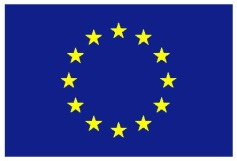
\includegraphics[width=1.07847in,height=0.73056in]{out-img2.jpg} } &
\multicolumn{1}{c}{

\includegraphics[width=1.27847in,height=0.88681in]{out-img3.jpg} } &
\multicolumn{1}{c}{

\includegraphics[width=1.30417in,height=1.06111in]{out-img4.png} }\\
\end{supertabular}
\end{flushleft}

\bigskip


\bigskip

\begin{flushleft}
\tablehead{}
\begin{supertabular}{|m{1.98856in}|m{4.25246in}|}
\hline
Project Acronym &
\bfseries Fed4FIRE\\\hline
Project Title &
\bfseries Federation for FIRE\\\hline
Instrument &
\bfseries Large scale integrating project (IP)\\\hline
Call identifier &
\bfseries FP7-ICT-2011-8\\\hline
Project number &
\bfseries 318389\\\hline
Project website &
\bfseries www.fed4fire.eu\\\hline
Experiment &
\bfseries GEO-Cloud\\\hline
\end{supertabular}
\end{flushleft}

\bigskip


\bigskip

{\centering\bfseries
Detailed Design Report
\par}


\bigskip

\begin{flushleft}
\tablehead{}
\begin{supertabular}{|m{1.9649599in}|m{4.27466in}|}
\hline
Work\ package &
WP10\\\hline
Task &
T10.1.2\ GEO-Cloud Experiment\\\hline
Due date &
10/01/2014\\\hline
Submission date &
10/01/2014\\\hline
Report Lead &
F\'elix Pedrera\ (DEIMOS)\\\hline
Version &
1.0\\\hline
Authors &
\foreignlanguage{spanish}{Manuel Jos\'e
Latorre}\foreignlanguage{spanish}{,\ }\foreignlanguage{spanish}{Antonio
Serrano G\'omez}\foreignlanguage{spanish}{, F\'elix Pedrera, Gerardo
Gonz\'alez, Jonathan
Becedas}\foreignlanguage{spanish}{\ (DEIMOS)}\foreignlanguage{dutch}{\ }\\\hline
Reviewers &
Jonathan Becedas\ (DEIMOS)\\\hline
\end{supertabular}
\end{flushleft}

\bigskip


\bigskip

\begin{flushleft}
\tablehead{}
\begin{supertabular}{|m{1.9649599in}|m{4.27466in}|}
\hline
\bfseries Document ID &
\selectlanguage{spanish}\bfseries GEO-Cloud-D10.8\\\hline
Abstract &
This document provides\ technical information about\ the GEO-Cloud
experiment detailed design\\\hline
Keywords &
Deliverable\\\hline
\end{supertabular}
\end{flushleft}

\bigskip


\bigskip

\begin{flushleft}
\tablehead{}
\begin{supertabular}{m{1.9649599in}|m{0.31495985in}|m{3.36706in}|m{0.43505988in}|}
\hline
\multicolumn{1}{|m{1.9649599in}|}{Nature of the\ document} &
R &
Report &
X\\\hline
 &
P &
Prototype &
~
\\\hhline{~---}
 &
D &
Demonstrator &
~
\\\hhline{~---}
 &
O &
Other &
~
\\\hline
\multicolumn{1}{|m{1.9649599in}|}{Dissemination level} &
PU &
Public &
~
\\\hline
 &
PP &
Restricted to other programme participants (including the Commission) &
~
\\\hhline{~---}
 &
RE &
Restricted to a group specified by the consortium (including the
Commision) &
~
\\\hhline{~---}
 &
CO &
Confidential, only for members of the consortium (including the
Commission) &
X\\\hhline{~---}
\end{supertabular}
\end{flushleft}

\bigskip

\clearpage
\textrm{\textbf{Disclaimer}}


\bigskip

\textit{The information, documentation and figures available in this
deliverable, is written by the Fed4FIRE\ }(Federation for
FIRE)\ \textit{{}-- project consortium under EC co-financing contract
FP7-ICT-}\textit{318389}\textit{\ and does not necessarily reflect the
views of the European Commission}\textit{. The European
C}\textit{ommission is not liable for any use that may be made of the
information contained herein.}

\clearpage
\textrm{\textbf{Executive S}}\textrm{\textbf{ummary}}


\bigskip

In this document the detailed design of the GEO-Cloud experiment is
presented. The document is divided into 7 sections:


\bigskip

Section\ 1\ introduces the document.


\bigskip

Section\ 2\ is devoted to the design of the satellite system. It is
constituted by the design of a constellation of 17 satellites and 12
ground stations. The satellites share the same orbit and take a world
land surface image on a daily basis. All the data generated is then
downloaded to the ground stations network.


\bigskip

Section\ 3\ presents\ the scenarios to be tested in the experiment. 6
use cases will be tested, although 11 were designed for its possible
implementation during the next stages of the experiment. Those use
cases are described in the Appendix included as Section\ 9.


\bigskip

Section\ 4\ describes the image distribution and visualization to
provide services through the BonFIRE cloud.


\bigskip

Section\ 5\ is devoted to the design of the architecture to be
implemented in BonFIRE, the processing chain of the
satellites{\textquoteright} images and the distribution of the the
image explained in Section 4.\ A first approach of the resources that
will be used in BonFIRE is included.


\bigskip

Section\ 6\ shows the design of the part of the experiment that will be
implemented in Virtual Wall and the connectivity required with BonFIRE.
A first approach of the resources that will be used in Virtual Wall is
included.


\bigskip

Section\ 7\ is devoted to the design of the experiment that will be
implemented and tested in PlanetLab Europe. A first approach of the
resources that will be used in Virtual Wall is included.


\bigskip

Section\ 8\ presents the cited bibliography throughout the text.


\bigskip

\clearpage
\textrm{\textbf{A}}\textrm{\textbf{cronyms and
A}}\textrm{\textbf{bbreviations}}


\bigskip

\begin{flushleft}
\tablehead{}
\begin{supertabular}{|m{0.8823598in}|m{5.35596in}|}
\hline
AOI &
Area of Interest\\\hline
API &
Application Programming Interface\\\hline
BF &
BonFIRE\\\hline
CDN &
Content Delivery Network\\\hline
CPU &
Central Processing Unit\\\hline
CSW &
Catalogue Services for the Web\\\hline
EaaS &
Elasticity as a Service\\\hline
EO &
Earth Observation\\\hline
ESDI &
European Spatial Data Infrastructure\\\hline
EUROGI &
European Umbrella Organization for Geographic Information\\\hline
EUROSUR &
European Border Surveillance System\\\hline
FGDC &
Federal Geographic Data Committee\\\hline
FTP &
File Transfer Protocol\\\hline
GIS &
Geographic Information System\\\hline
GMES &
Global Monitoring for Environment and Security\\\hline
GPS &
Global Positioning System\\\hline
GPU &
Graphics Processing Unit\\\hline
GQ &
Golden Quadrilateral\\\hline
GS &
Ground Station\\\hline
GSD &
Ground Sample Distance\\\hline
HMA &
Heterogeneous Missions Accessibility\\\hline
HPC &
High Performance Computing\\\hline
HTTP &
Hypertext Transfer Protocol\\\hline
INSPIRE &
Infrastructure for Spatial Information in Europe\\\hline
ISO &
International Organization for Standardization\\\hline
KML &
Keyhole Markup Language\\\hline
L0 &
Level 0 processor\\\hline
L1A\  &
Level 1 A processor\\\hline
L1B &
Level 1 B processor\\\hline
L1C &
Level 1 C processor\\\hline
LEO &
Low Earth Orbit\\\hline
LTAN &
Local Time of Ascending Node\\\hline
NASA &
National Aeronautics and Space Administration\\\hline
NHAI &
National Highways Authority of India\\\hline
OGC &
Open Geospatial Consortium\\\hline
PNOT &
Plan Nacional de Observaci\'on del Territorio (Spanish Plan of Territory
Observation and Urbanism)\\\hline
PNT &
Plan Nacional de Teledetecci\'on (Spanish Plan of Remote
Sensing)\\\hline
PP &
Product Processor\\\hline
RDBMS &
Relational Database Management System\\\hline
REST &
Representational State Transfer\\\hline
Sat &
Satellite\\\hline
SCO &
Snow Cover Area\\\hline
SDI &
Spatial Data Infrastructure\\\hline
SFTP &
Secure File Transfer Protocol\\\hline
SOA &
Service Oriented Architecture\\\hline
SQL &
Structured Query Language\\\hline
SSO &
Sun-Synchronous Orbit\\\hline
SWE &
Snow Water Equivalent\\\hline
TBD &
To be defined\\\hline
TMS &
Tile Map Service\\\hline
UAV &
Unmanned Aerial Vehicle\\\hline
VM &
Virtual Machine\\\hline
VW &
Virtual Wall\\\hline
WCS &
Web Coverage Service\\\hline
WFS &
Web Feature Service\\\hline
WMS &
Web Map Service\\\hline
WMS-C &
Web Map Tile Caching\\\hline
WMTS &
Web Map Tile Service\\\hline
WPS &
Web Processing Service\\\hline
WS &
Web Service\\\hline
XML &
eXtensible Markup Language\\\hline
\end{supertabular}
\end{flushleft}
\clearpage
\textrm{\textbf{Table of C}}\textrm{\textbf{ontents}}


\bigskip

\setcounter{tocdepth}{3}
\tableofcontents

\bigskip

\section[Introduction]{Introduction}
\label{bkm:Ref378931869}\hypertarget{Toc381777184}{}\label{bkm:Ref378929304}
\bigskip

The GEO-Cloud experiment consists of the emulation of a realistic and
complete Earth Observation System that provides services using cloud
technology. For that purpose a constellation of satellites, ground
stations, a cloud architecture, use cases and end
users{\textquoteright} models are designed.


\bigskip

The EO system will be computed and emulated in Fed4FIRE: A constellation
of satellites record images of the Earth in a daily basis. The images
are transferred to ground stations that ingest the data into a cloud
computing infrastructure. The data is processed and distributed to end
users.


\bigskip

The GEO-Cloud experiment is tested in three testbeds: Virtual Wall,
BonFIRE and PlanetLab Europe. GEO-Cloud is divided into two
sub-experiments:

\liststyleLFOxli
\begin{itemize}
\item One experiment in a system integrated in Virtual Wall and BonFIRE.
\item One experiment in PlanetLab Europe.
\end{itemize}
The experiment in Virtual Wall and BonFIRE emulates the whole EO system.
In Virtual Wall: constellation of satellites, the ground stations and
the end users{\textquoteright} models. In BonFIRE the cloud
architecture, the processing chain of the data and its distribution.
Both Virtual Wall and BonFIRE are interconnected to transfer
information from one testbed to the other and viceversa.


\bigskip

The experiment in PlanetLab Europe consists of the emulation of the
networks that constitute the links between the ground stations to the
cloud and from the cloud to the end users. There, the network
performance, features, bandwidth and impairments are monitored and
measured. Those parameters once measured are used to update the models
implemented in Virtual Wall, i.e, bandwidth, latency, loss rate and
background noise.


\bigskip

In the next sections, the detailed design of the GEO-Cloud experiment is
introduced.

\section[Satellite System Design]{Satellite System Design}
\label{bkm:Ref378931876}\hypertarget{Toc381777185}{}
\bigskip

\subsection[Design of the flight and ground segments]{Design of the
flight and ground segments}
\hypertarget{Toc381777186}{}In this section, the main characteristics of
the system are presented. Objectives, constraints, previous estimations
and possible modifications and their effects in the system are exposed.


\bigskip

In a wide vision, it is an\ \textbf{Earth Observation (EO)}\ system
consisting\ of\ a constellation of satellites equally spaced in a LEO
orbit\ with the aim of achieving\ \textbf{daily coverage}\ of the
entire Earth\ surface. These conditions imply a very sophisticated
handle of a huge quantity of data.


\bigskip

The following requirements\ have\ been fulfilled to design the system:

\liststyleLFOiii
\setcounter{saveenum}{\value{enumi}}
\begin{enumerate}
\setcounter{enumi}{\value{saveenum}}
\item Swath: 160km (based on state of the art cameras).
\item Resolution: 6.7m (based on state of the art cameras).
\item Low Earth Orbits.
\item Sun Synchronous orbits.\ 
\item Download data rate: 160 Mbps (based on Deimos-2 satellite
characteristics).
\item Optical Bands: 5 Multispectral (based on state of the art
cameras).
\end{enumerate}

\bigskip


\bigskip

\subsubsection[Global Daily Coverage]{Global Daily Coverage}
\hypertarget{Toc381777187}{}The objective of this system is the
acquisition of images of the\ total\ Earth\ surface in a daily basis.
Global coverage is considered to include the land surface that is shown
in\ Figure 1.


\bigskip

{\centering 
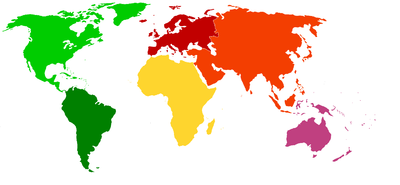
\includegraphics[width=4.26944in,height=1.93056in]{out-img5.png} \par}

\begin{center}
\tablehead{}
\begin{supertabular}{m{0.8316598in}m{0.49065986in}m{0.67535985in}m{0.5906598in}m{0.73715985in}}
\hline
\centering
\textbf{\textcolor{black}{~~~}}\textbf{\textcolor{black}{~~~}}\textbf{\textcolor{black}{~}}\href{http://es.wikipedia.org/wiki/Am?rica}{\textbf{\textcolor[rgb]{0.043137256,0.0,0.5019608}{America}}}
&
\textbf{\textcolor{black}{~~~}}\textbf{\textcolor{black}{~}}\href{http://es.wikipedia.org/wiki/Asia}{\textbf{\textcolor[rgb]{0.043137256,0.0,0.5019608}{Asia}}}
&
\textbf{\textcolor{black}{~~~}}\textbf{\textcolor{black}{~}}\href{http://es.wikipedia.org/wiki/Europa}{\textbf{\textcolor[rgb]{0.043137256,0.0,0.5019608}{Europ}}}\textbf{\textcolor{black}{e}}
&
\textbf{\textcolor{black}{~~~}}\textbf{\textcolor{black}{~}}\href{http://es.wikipedia.org/wiki/?frica}{\textbf{\textcolor[rgb]{0.043137256,0.0,0.5019608}{Africa}}}
&
\textbf{\textcolor{black}{~~~}}\textbf{\textcolor{black}{~}}\href{http://es.wikipedia.org/wiki/Ocean?a}{\textbf{\textcolor[rgb]{0.043137256,0.0,0.5019608}{Oceania}}}\\\hline
\end{supertabular}
\end{center}
{\centering\bfseries
\label{bkm:Ref376877604}Figure\ 1.\ Land surface to be acquired\ in a
daily basis.
\par}


\bigskip

This plan of acquisition implies the system to be able of\ taking a
volume
of\ image\ higher\ than\ \textbf{135}\textbf{\ }\foreignlanguage{english}{\textbf{M}}\foreignlanguage{english}{\textbf{illions}}\textbf{\ km}\textbf{\textsuperscript{2}}\textbf{\ per
day}, as\ shown in\ Table 1.


\bigskip

{\centering\bfseries
\label{bkm:Ref377037137}Table\ 1. Surface of each continent.
\par}

\begin{center}
\tablehead{}
\begin{supertabular}{m{0.71985984in}m{1.0364599in}}
\hline
\bfseries\color{black} Continent &
\raggedleft\arraybslash \bfseries\color{black} Surface
(km{\texttwosuperior})\\\hline
\href{http://es.wikipedia.org/wiki/Asia}{\textbf{\textcolor[rgb]{0.043137256,0.0,0.5019608}{Asia}}}
&
\raggedleft\arraybslash \color{black} 43~810~000\\
\href{http://es.wikipedia.org/wiki/Am?rica}{\textbf{\textcolor[rgb]{0.043137256,0.0,0.5019608}{America}}}
&
\raggedleft\arraybslash \color{black} 42~330~000\\
\href{http://es.wikipedia.org/wiki/?frica}{\textbf{\textcolor[rgb]{0.043137256,0.0,0.5019608}{Africa}}}
&
\raggedleft\arraybslash \color{black} 30~370~000\\
\href{http://es.wikipedia.org/wiki/Europa}{\textbf{\textcolor[rgb]{0.043137256,0.0,0.5019608}{Europ}}}\textbf{\textcolor{black}{e}}
&
\raggedleft\arraybslash \color{black} 10~180~000\\
\href{http://es.wikipedia.org/wiki/Ocean?a}{\textbf{\textcolor[rgb]{0.043137256,0.0,0.5019608}{Oceania}}}
&
\raggedleft\arraybslash \color{black} 9~008~500\\
\textbf{\textcolor[rgb]{0.043137256,0.0,0.5019608}{TOTAL}} &
\raggedleft\arraybslash \color{black} 135 698 500\\\hline
\end{supertabular}
\end{center}

\bigskip

This acquisition plan is used\ for the mission\ because it is very
demanding in terms of data handling.\ 


\bigskip

{\itshape
In the experiment we will define\ scenarios with\ areas of interest in
order to reduce the amount of data processed, stored and distributed
through the Fed4FIRE infrastructure.\ }


\bigskip

\subsubsection[Flight Segment]{Flight Segment}
\hypertarget{Toc381777188}{}The satellites are selected according to the
current state of the art.\ However, some enhancements can be assumed as
a way to adjust the analysis to the short term future.


\bigskip

\paragraph[Satellite\ performances]{Satellite\ performances}
As a first iteration for the system, small platforms of less of 500kg
are supposed according to the size and payload bay characteristics of
representative platforms in this category. This study is based on the
bus platforms currently offered by\ Surrey Satellite Technology Ltd,
Satrec Initiative, Sierra Nevada Corporation, etcetera.\ 


\bigskip

To reduce the amount of satellites orbiting the Earth, a design
with\ two payloads has been\ assumed.\ Thus,\ the swath (the width of
the\ field of view of\ each\ satellite\ in the surface of the Earth)
can be duplicated\ without decreasing the resolution.


\bigskip

The satellites shall be\ \textbf{pointing to nadir}, acquiring images
without maneuvering because of the acquisition plan for cover the
Earth\ daily. Simultaneously, when a satellite\ gets\ into the field of
view of a Ground Station, the download starts\ and\ at the same time
the satellite continues imaging.


\bigskip

The main specifications of the satellites in the constellation are shown
in\ Table 2.\ The values of each parameter have been selected according
to the state of the art and the desired quality of the images in the
mission.

{\centering\bfseries
\label{bkm:Ref377037648}Table\ 2. Main performances of the satellites.
\par}

\begin{center}
\tablehead{}
\begin{supertabular}{m{1.3906599in}m{0.7587598in}}
\hline
\bfseries\color{black} Specification &
\raggedleft\arraybslash \bfseries\color{black} Value\\\hline
\bfseries\color[rgb]{0.043137256,0.0,0.5019608} GSD &
\raggedleft\arraybslash \color{black} 6.7 m\\
\bfseries\color[rgb]{0.043137256,0.0,0.5019608} Swath &
\raggedleft\arraybslash \color{black} 160 km\\
\bfseries\color[rgb]{0.043137256,0.0,0.5019608} Number of bands &
\raggedleft\arraybslash \color{black} 5\\
\bfseries\color[rgb]{0.043137256,0.0,0.5019608} Digitalization &
\raggedleft\arraybslash \color{black} 12 bits\\
\bfseries\color[rgb]{0.043137256,0.0,0.5019608} Download data rate &
\raggedleft\arraybslash \color{black} 160 Mbps\\
\bfseries\color[rgb]{0.043137256,0.0,0.5019608} Compression rate &
\raggedleft\arraybslash \color{black} 2:1\\\hline
\end{supertabular}
\end{center}

\bigskip

{\itshape
Some\ options to\ reduce the acquired data, apart from\ defining
scenarios and areas of interest are the following:}

\liststyleLFOii
\begin{itemize}
\item {\itshape
To reduce the resolution\ by increasing\ the value of the GSD. This\ has
a strong impact in the quality of the images and therefore in the
mission.}
\item {\itshape
To decrease the number of bands, this reduces the spectral information
that is acquired in each image.}
\item {\itshape
To change the digitalization of the pixels from 12bits to 8bits,
10bits{\dots} which has an impact in the quality of the image too by
reducing the information included in each pixel.}
\item {\itshape
To enhance the ratios of compression to reduce the size of the
compressed images before the download. 2:1 is an average\ ratio for
lossless compression, but the use of lossy compression\ (with variable
ratios depending on\ the image) is also extended reaching to ratios up
to 100 times of reduction of the original size in the most favorable
cases\ (clouds, sea{\dots}).}
\end{itemize}

\bigskip

\textit{Changes in the swath only affects to the number of required
satellites to cover the Earth, as can be seen
in}\textit{\ Section}\textit{\ }\textit{2.1.2.3}\textit{.}


\bigskip

{\itshape
The download data rate is also an adjustable parameter\ that affects to
the time the satellites have to be downloading the acquired data. If
data rate increases, the number of ground stations for the reception of
images could be reduced.}


\bigskip

\paragraph[Orbit\ definition]{Orbit\ definition}
It is common in\ EO\ satellite missions the use
of\ \textbf{sun-synchronous}\textbf{\ }orbits.\ These\ orbits
guarantee\ that the\ lighting conditions of the imaged places\ are\ the
same during the mission, which is a very desirable characteristic.\ 


\bigskip

LTAN\ (Local Time Ascending Node)\ is also a\ desired\ condition of the
orbit very related to the\ lighting and weather
conditions\ of\ those\ places\ that\ the satellite overflies\ (LTAN is
selected according to the desired\ local time of the overflown places
and the cloud formation\ during the day); it is common\ the use
of\ \textbf{LTAN 10:30h}\textbf{\ }for Earth Observation.\ 


\bigskip

Other of the main parameters of an orbit is the altitude. Altitude has
effects in the resolution and the\ swath\ of the satellites, which has
impact in the number of satellites required to achieve the coverage
objective. According to the\ value of those parameters in the payloads
included in the satellites, the reference altitude for the system\ was
found to be\ \textbf{646km}.\ Sun-Synchronous Orbit (SSO)\ condition
implies a relation between the altitude and the inclination of the
orbit of\ \textbf{97.97}\textbf{deg}\ in this case.


\bigskip

{\itshape
Changes in the altitude of the orbit have strong effects in main
parameters\ of the mission. When altitude is increased resolution
worsens but swath increases too, then the number of satellites could be
reduced and the data volume would be lower.\ Consequently,
if\ the\ altitude\ decreases the\ resolution\ and the\ data
volume\ increase\ whilst the swath is reduced and then more satellites
would be required.}


\bigskip

\paragraph[Number of satellites in the constellation]{Number of
satellites in the constellation}
\label{bkm:Ref376938057}
\bigskip

In this section, the strategy for covering\ the Earth\ in
a\ daily\ basis\ is explained. The result of the calculation is the
required number of satellites in the orbit and the gap between them in
the orbit.\ 

Taking advantage of the\ geometry\ that\ the problem involves, it is
easy to achieve a pattern which is repeated\ in\ each orbit. This
pattern consists of\ overlapping\ the swath of each satellite with the
swath of the next satellite in the orbit by adjusting the distance
between them. In\ Figure 2\ it\ can be seen the whole pattern, it
progresses over the surface of the\ Earth in consecutive orbits
covering it completely\ in one day.

{\centering 
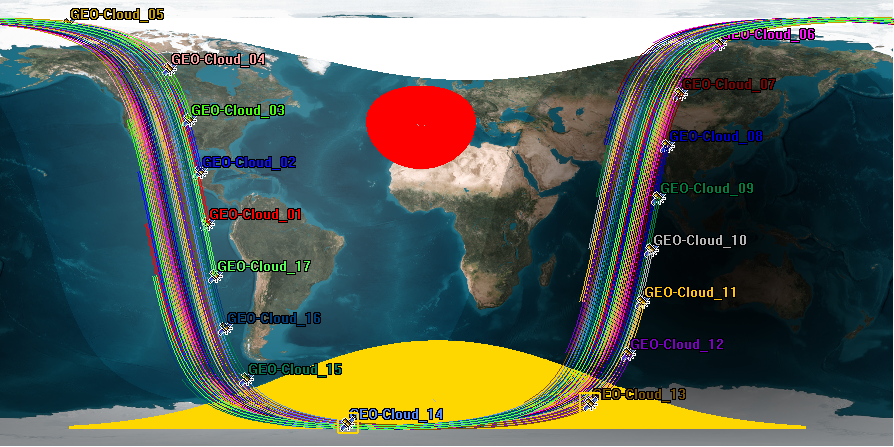
\includegraphics[width=3.47846in,height=2.87843in]{out-img6.png} \par}

{\centering\bfseries
\label{bkm:Ref376945910}Figure\ 2. Pattern of overlapped swaths in one
orbit.
\par}


\bigskip

The number of satellites and the distance between them shall be
calculated from the following inputs in\ Table 3.


\bigskip

{\centering\bfseries
\label{bkm:Ref377038544}Table\ 3. Inputs for the calculation of the the
number of satellites.
\par}

\begin{center}
\tablehead{}
\begin{supertabular}{m{0.8212598in}m{0.7663598in}}
\hline
\bfseries\color{black} Inputs &
\raggedleft\arraybslash \bfseries\color{black} Value\\\hline
\bfseries\color[rgb]{0.043137256,0.0,0.5019608} Altitude &
\raggedleft\arraybslash \color{black} 646 km\\
\bfseries\color[rgb]{0.043137256,0.0,0.5019608} Inclination &
\raggedleft\arraybslash \color{black} 97.97 deg\\
\bfseries\color[rgb]{0.043137256,0.0,0.5019608} Swath\  &
\raggedleft\arraybslash \color{black} 160 km\\\hline
\end{supertabular}
\end{center}

\bigskip

To achieve the overlapped swathes in a SSO,\ the satellites shall be
placed\ taking into account that\ the Earth rotates a distance between
passes over the equator of consecutive\ satellites that makes their
swaths overlap.\ At higher latitudes, the swaths are more
overlapped\ and this is why the equator is the most\ restrictive case
and where the calculations are made. For these orbits\ and swath,
the\ number of satellites obtained to carry out this mission is 17,
(see\ Table 4).


\bigskip

{\centering\bfseries
\label{bkm:Ref377038810}Table\ 4. Required number of satellites.
\par}

\begin{center}
\tablehead{}
\begin{supertabular}{m{1.3837599in}m{0.93645984in}}
\hline
\bfseries\color{black} Outputs &
\raggedleft\arraybslash \bfseries\color{black} Value\\\hline
\bfseries\color[rgb]{0.043137256,0.0,0.5019608} Required satellites &
\raggedleft\arraybslash \color{black} 17 satellites\\\hline
\end{supertabular}
\end{center}

\bigskip

The orbit period is directly calculated with the value of
altitude.\ Adding the number of satellites, it\ is calculated the
distance they have to be spaced and shown in\ Table 5.


\bigskip

{\centering\bfseries
\label{bkm:Ref377038819}Table\ 5.\ Period and space between consecutive
satellites in orbit.
\par}

\begin{center}
\tablehead{}
\begin{supertabular}{m{2.7114599in}m{0.8357598in}}
\hline
\bfseries\color{black} Outputs &
\raggedleft\arraybslash \bfseries\color{black} Value\\\hline
\bfseries\color[rgb]{0.043137256,0.0,0.5019608} Period &
\raggedleft\arraybslash \color{black} 97.50\ min\\
\bfseries\color[rgb]{0.043137256,0.0,0.5019608} Time between satellites
in the orbit &
\raggedleft\arraybslash \color{black} 5.74 min\\
\bfseries\color[rgb]{0.043137256,0.0,0.5019608} Distance between
satellites in the orbit &
\raggedleft\arraybslash \color{black} 2593.48km\\\hline
\end{supertabular}
\end{center}

\bigskip

In\ Figure 3\ the whole constellation\ of satellites is shown.

{\centering 
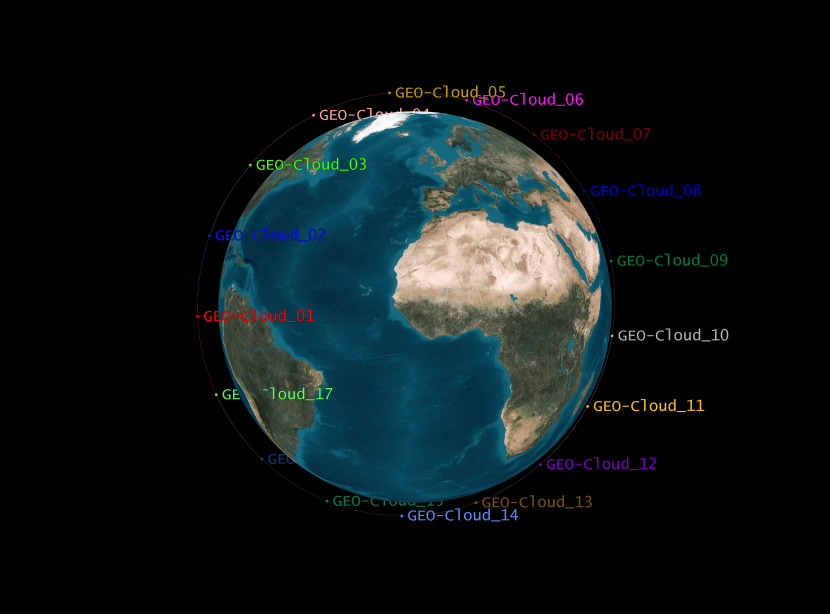
\includegraphics[width=3.76528in,height=2.79097in]{out-img7.png} \par}

{\centering\bfseries
\label{bkm:Ref376947064}Figure\ 3.\ Constellation of 17 satellites in a
SSO orbit\ at 646km.
\par}

\subsubsection[Ground\ stations design]{Ground\ stations design}
\hypertarget{Toc381777189}{}When the satellite\ acquires the data, it
has to be downloaded to the Ground Stations and then\ it has to
be\ distributed\ to the customers.\ Due to the huge quantity of data
and the limitations the download data rate sets, several stations
distributed over the surface of the Earth\ are required.
They\ will\ allow the satellite to communicate with them\ and download
the images.\ 


\bigskip

The accumulated duration of the accesses\ to all the ground
stations\ per day is the parameter\ used\ to\ calculate\ how many
stations are included and where they\ should be\ located.\ 


\bigskip

The frequency of accesses per day varies with the latitude of the
station, being Svalbard at the North Pole the ground station with more
accesses per day, one per orbit.\ In\ Table 6, the ground stations
chosen for the mission, with the number of accesses and duration of the
passes by satellite are depicted.

{\centering\bfseries
\label{bkm:Ref377044034}Table\ 6\ Ground stations design, number of
accesses per day and duration of the passes.
\par}

\begin{center}
\tablehead{\hline
\bfseries\color{black} Ground Station &
\bfseries\color{black} Accesses per day &
\bfseries\color{black} Accumulated duration (h)\\\hline}
\begin{supertabular}{m{0.98095983in}m{0.6288598in}m{0.90525985in}}
\bfseries\color{black} Irkutsk &
\raggedleft \color{black} 7 &
\raggedleft\arraybslash \color{black} 0.95\\
\bfseries\color{black} Puertollano &
\raggedleft \color{black} 4 &
\raggedleft\arraybslash \color{black} 0.62\\
\bfseries\color{black} Svalbard &
\raggedleft \color{black} 15 &
\raggedleft\arraybslash \color{black} 2.21\\
\bfseries\color{black} Troll &
\raggedleft \color{black} 11 &
\raggedleft\arraybslash \color{black} 1.69\\
\bfseries\color{black} Chetumal &
\raggedleft \color{black} 3 &
\raggedleft\arraybslash \color{black} 0.50\\
\bfseries\color{black} Cordoba &
\raggedleft \color{black} 4 &
\raggedleft\arraybslash \color{black} 0.53\\
\bfseries\color{black} Dubai &
\raggedleft \color{black} 4 &
\raggedleft\arraybslash \color{black} 0.57\\
\bfseries\color{black} Kourou &
\raggedleft \color{black} 4 &
\raggedleft\arraybslash \color{black} 0.49\\
\bfseries\color{black} Krugersdorp &
\raggedleft \color{black} 4 &
\raggedleft\arraybslash \color{black} 0.54\\
\bfseries\color{black} Malaysia &
\raggedleft \color{black} 3 &
\raggedleft\arraybslash \color{black} 0.42\\
\bfseries\color{black} Prince Albert &
\raggedleft \color{black} 6 &
\raggedleft\arraybslash \color{black} 0.93\\
\bfseries\color{black} Sidney &
\raggedleft \color{black} 4 &
\raggedleft\arraybslash \color{black} 0.61\\\hline
\bfseries\color{black} TOTAL &
\raggedleft \bfseries\color{black} 69 &
\raggedleft\arraybslash \bfseries\color{black} 10.07\\\hline
\end{supertabular}
\end{center}

\bigskip

In\ Figure 4\ the footprints (area in which the satellites can
communicate with the ground stations) of the selected ground stations
are depicted.


\bigskip

{\centering 
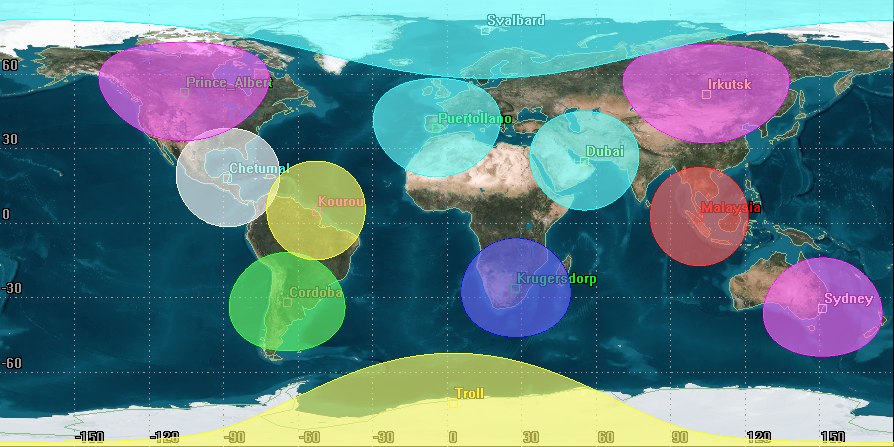
\includegraphics[width=6.29861in,height=3.14931in]{out-img8.png} \par}

{\centering\bfseries
\label{bkm:Ref377044167}Figure\ 4.\ Footprints of the selected Ground
Stations.
\par}


\bigskip

\subsection[Generated\ Data\ Volume]{Generated\ Data\ Volume}
\hypertarget{Toc381777190}{}Almost\ 136M
km\textsuperscript{2}/day\ are\ daily\ acquired. With the following
expression can\ estimate\ the data volume\ generated:

{\centering \par}

Before downloading the images they are compressed. The\ ancillary data
is included in the process (auxiliary information useful for the
geolocation of the images, protocols{\dots}). In this case, the
ancillary data is estimated\ to be\ 12\% of the acquired data\ (based
on Deimos 2 satellite measurements), which is added and then
compressed. With the values\ depicted in\ Table 7\ the\ data on ground
can be estimated.


\bigskip

{\centering\bfseries
\label{bkm:Ref377044461}Table\ 7. Data handling parameters.
\par}

\begin{center}
\tablehead{}
\begin{supertabular}{m{1.3906599in}m{1.3302599in}}
\hline
\bfseries\color{black} Parameter &
\raggedleft\arraybslash \bfseries\color{black} Value\\\hline
\bfseries\color[rgb]{0.043137256,0.0,0.5019608} Daily acquisition &
\raggedleft\arraybslash \textcolor{black}{135 698
500}\textcolor{black}{\ km}\textcolor{black}{\textsuperscript{2}}\\
\bfseries\color[rgb]{0.043137256,0.0,0.5019608} GSD &
\raggedleft\arraybslash \color{black} 6.7 m\\
\bfseries\color[rgb]{0.043137256,0.0,0.5019608} Number of bands &
\raggedleft\arraybslash \color{black} 5\\
\bfseries\color[rgb]{0.043137256,0.0,0.5019608} Digitalization &
\raggedleft\arraybslash \color{black} 12 bits\\
\bfseries\color[rgb]{0.043137256,0.0,0.5019608} Ancillary data &
\raggedleft\arraybslash \color{black} 12\%\\
\bfseries\color[rgb]{0.043137256,0.0,0.5019608} Compression rate &
\raggedleft\arraybslash \color{black} 2:1\\
\bfseries\color[rgb]{0.043137256,0.0,0.5019608} Download data rate &
\raggedleft\arraybslash \color{black} 160 Mbps\\\hline
\end{supertabular}
\end{center}

\bigskip


\bigskip

By including\ ancillary
data\ before\ compression,\ \textbf{1}\textbf{1.}\textbf{55}\textbf{TBytes}\ shall
be downloaded daily.\ According to the number of satellites in the
system and the download data rate,\ \textbf{each
satellite}\ \textbf{will}\textbf{\ }\textbf{download}\textbf{\ }\textbf{images
during\ }\textbf{9.89h}\textbf{/}\textbf{day}\textbf{.\ }This would
provide all the acquired date on ground in a daily basis.


\bigskip

With the selected Ground Stations, the\ maximum allowed\ duration of all
accesses of a satellite in a day\ can be calculated:\ \textbf{10.07h/
day}\ at 160Mbps.\ 


\bigskip

\subsection[Summary]{Summary}
\hypertarget{Toc381777191}{}To summarize, performances and results of
this report are collected in\ Table 8.


\bigskip

{\centering\bfseries
\label{bkm:Ref377045498}Table\ 8.\ Performances and results.
\par}

\begin{center}
\tablehead{}
\begin{supertabular}{m{1.3260599in}m{1.4962599in}m{1.1267599in}}
\hline
~
 &
\bfseries\color{black} Parameter &
\raggedleft\arraybslash \bfseries\color{black} Value\\\hline
\centering \bfseries\color[rgb]{0.043137256,0.0,0.5019608} SATELLITE
PERFORMANCES &
\color[rgb]{0.043137256,0.0,0.5019608} Daily acquisition &
\raggedleft\arraybslash \textcolor{black}{135 698 500
km}\textcolor{black}{\textsuperscript{2}}\\
 &
\color[rgb]{0.043137256,0.0,0.5019608} GSD &
\raggedleft\arraybslash \color{black} 6.7 m\\
 &
\color[rgb]{0.043137256,0.0,0.5019608} Swath &
\raggedleft\arraybslash \color{black} 160 km\\
 &
\color[rgb]{0.043137256,0.0,0.5019608} Number of bands &
\raggedleft\arraybslash \color{black} 5\\
 &
\color[rgb]{0.043137256,0.0,0.5019608} Digitalization &
\raggedleft\arraybslash \color{black} 12 bits\\
 &
\color[rgb]{0.043137256,0.0,0.5019608} Ancillary data &
\raggedleft\arraybslash \color{black} 12\%\\
 &
\color[rgb]{0.043137256,0.0,0.5019608} Compression rate &
\raggedleft\arraybslash \color{black} 2:1\\
 &
\color[rgb]{0.043137256,0.0,0.5019608} Download data rate &
\raggedleft\arraybslash \color{black} 160 Mbps\\
~
 &
~
 &
~
\\
\centering \bfseries\color[rgb]{0.043137256,0.0,0.5019608} CONSTELLATION
DESIGN &
\color[rgb]{0.043137256,0.0,0.5019608} Number of satellites &
\raggedleft\arraybslash \color{black} 17 satellites\\
 &
\color[rgb]{0.043137256,0.0,0.5019608} Orbit altitude &
\raggedleft\arraybslash \color{black} 646 km\\
 &
\color[rgb]{0.043137256,0.0,0.5019608} Inclination &
\raggedleft\arraybslash \color{black} 97.97 deg\\
 &
\color[rgb]{0.043137256,0.0,0.5019608} LTAN &
\raggedleft\arraybslash \color{black} 10:30 h\\
~
 &
~
 &
~
\\
\centering \bfseries\color[rgb]{0.043137256,0.0,0.5019608} GROUND
STATIONS &
\color[rgb]{0.043137256,0.0,0.5019608} Number of G/S &
\raggedleft\arraybslash \color{black} 12\\
 &
\color[rgb]{0.043137256,0.0,0.5019608} Average accesses per day for each
satellite &
\raggedleft\arraybslash \color{black} 69\\
 &
\color[rgb]{0.043137256,0.0,0.5019608} Average duration of all the
accesses per day for each satellite &
\raggedleft\arraybslash \color{black} 10.07 h\\
~
 &
\textbf{Parameter} &
\raggedleft\arraybslash \textbf{Value}\\
\centering \bfseries\color[rgb]{0.043137256,0.0,0.5019608} DATA VOLUME &
\color[rgb]{0.043137256,0.0,0.5019608} Total downloaded data per day &
\raggedleft\arraybslash \color{black} 11.55 TBytes\\\hhline{-~~}
 &
\color[rgb]{0.043137256,0.0,0.5019608} Downloaded data per day for each
satellite &
\raggedleft\arraybslash \color{black} 695.72 GBytes\\
 &
\color[rgb]{0.043137256,0.0,0.5019608} Time of downloading per day for
each satellite &
\raggedleft\arraybslash \color{black} 9.89 h\\\hhline{~--}
\end{supertabular}
\end{center}

\bigskip


\bigskip

\section[Scenarios definition and users{\textquoteright} model
design]{Scenarios definition and users{\textquoteright} model design}
\label{bkm:Ref378929303}\label{bkm:Ref378929308}\label{bkm:Ref378929368}\label{bkm:Ref378929383}\hypertarget{Toc381777192}{}
\bigskip

In\ this section\ technical information about the scenarios and the
models of the end users to be tested in the GEO-Cloud experiment are
provided.


\bigskip

With the designed scenarios we intend to widely cover several
applications that fit the resolution, revisit time, spectral
bands{\dots} of the designed satellite system.\ 


\bigskip

As seen in\ Figure 5\ and\ Figure 6, the applications in which satellite
imagery is used are related with the spectral bands of the payload, the
revisit time and the resolution of the images. In GEO-Cloud, we defined
daily revisit time and a multispectral payload with a resolution below
10m.


\bigskip

The applications that can be covered by the GEO-Cloud system are the
following:\ \textit{h}\textit{ydrology,\ }\textit{a}\textit{griculture,\ }\textit{e}\textit{nvironmental\ }\textit{m}\textit{onitoring,\ }\textit{i}\textit{ntelligence,\ }\textit{u}\textit{rban\ }\textit{d}\textit{evelopment}\textit{\ and
infrastructures
monitoring}\textit{,\ }\textit{m}\textit{apping,\ }\textit{land
management (topology, geology, forestry), disaster monitoring and
maritime surveillance.}


\bigskip

Other application such as traffic is out of scope because of the very
high-resolution requirement (1m). Oceanography is also out of scope
because we only consider for GEO-Cloud land surface and not oceans.
Meteorology is out of scope because it is covered by geostationary
systems, which resolution is between 100 m and 8000 m. However we do
consider meteorology based in low Earth orbit satellites for some
applications such as precision agriculture or hydrology.


\bigskip

{\centering 
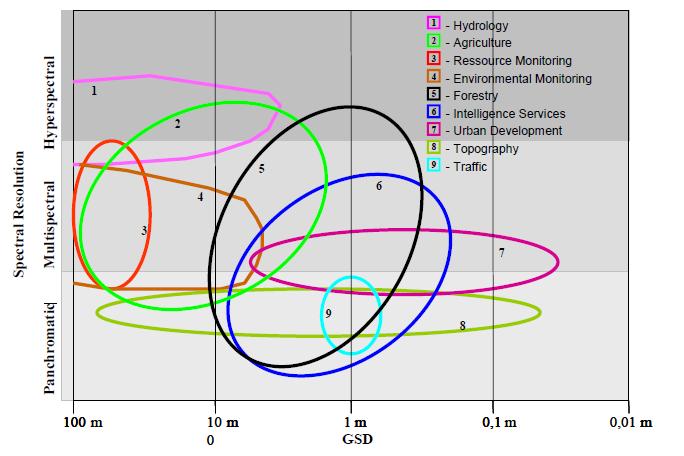
\includegraphics[width=4.18585in,height=2.79056in]{out-img9.png} \par}

{\centering\bfseries
\label{bkm:Ref377564516}Figure\ 5.\ Earth observation request: GSD
versus spectral resolution\ (From\ (Sandau)).
\par}


\bigskip

{\centering 
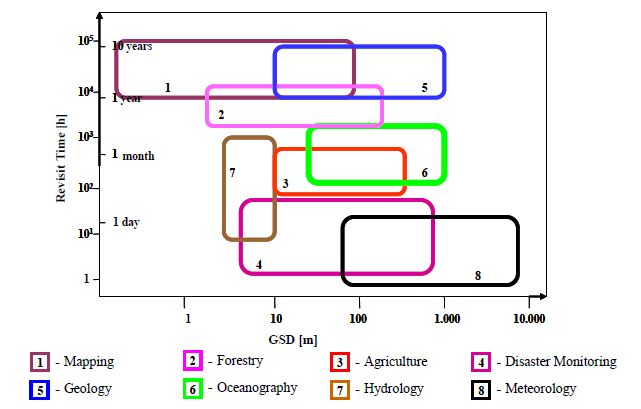
\includegraphics[width=4.69218in,height=2.9938in]{out-img10.png} \par}

{\centering\bfseries
\label{bkm:Ref377564518}Figure\ 6.\ Earth observation request: GSD vs
revisit time\ (From\ (Sandau)).
\par}


\bigskip

Trying to cover\ most of\ these fields, the following scenarios have
been designed:


\bigskip

\liststyleLFOxi
\begin{itemize}
\item Scenario 1:\ \foreignlanguage{english}{Emergencies - Lorca
Earthquake (Spain)}
\item Scenario\ 2:\ \foreignlanguage{english}{Infrastructure monitoring
- Affection in railway infrastructures by sand movement in desert areas
(Spain)}
\item Scenario 3: Land Management -- South West of England.
\item Scenario 4: Precision Agriculture -- Argentina.
\item Scenario 5:\ Basemaps -- Wordlwide.
\item Scenario 6: Online Catalogue / Ordering -- Worldwide.
\end{itemize}
End users are also designed and described for each scenario along with
the diagram shown in\ Table 9. In this diagram the service type,
processing, storage and communications loads and demand variability are
defined.

\clearpage
\bigskip


\bigskip

{\centering\bfseries
\label{bkm:Ref377566016}Table\ 9. Relation of the users demand with the
service offered.
\par}

\begin{center}
\tablehead{}
\begin{supertabular}{m{0.53165984in}m{0.92955977in}m{0.68855983in}|m{1.0649599in}m{1.1274599in}|m{0.6718598in}m{0.21425986in}}
\hhline{~-----~}
\multicolumn{1}{m{0.53165984in}|}{~
} &
\multicolumn{2}{m{1.6968598in}|}{\centering
\selectlanguage{spanish}\bfseries\color{black} Service Type} &
\multicolumn{2}{m{2.27116in}|}{\centering
\selectlanguage{spanish}\bfseries\color{black} Loads in Cloud
Technology} &
\multicolumn{1}{m{0.6718598in}|}{\selectlanguage{spanish}\bfseries\color{black}
Demand Variability} &
~
\\\hline
\multicolumn{1}{|m{0.53165984in}|}{\centering
\selectlanguage{spanish}\bfseries\color{black}
COMPANY{\textquotesingle}S SERVICES} &
\multicolumn{1}{m{0.92955977in}|}{\centering
\selectlanguage{spanish}\color{black} Basic} &
\centering \selectlanguage{spanish}\color{black} Basic &
\multicolumn{1}{m{1.0649599in}|}{\centering
\selectlanguage{spanish}\color{black} Processing} &
\centering \selectlanguage{spanish}\color{black} Low &
\multicolumn{1}{m{0.6718598in}|}{\centering
\selectlanguage{spanish}\color{black} Constant} &
\multicolumn{1}{m{0.21425986in}|}{\centering\arraybslash
\selectlanguage{spanish}\bfseries\color{black} USERS{\textquotesingle}
DEMAND}\\\hline
 &
 &
 &
 &
\centering \selectlanguage{spanish}\color{black} Medium &
 &
\\\hhline{~~~~-~~}
 &
 &
\centering \selectlanguage{spanish}\color{black} Advanced &
 &
\centering \selectlanguage{spanish}\color{black} High &
 &
\\\hhline{~~-~-~~}
 &
 &
 &
\multicolumn{1}{m{1.0649599in}|}{\centering
\selectlanguage{spanish}\color{black} Storage} &
\centering \selectlanguage{spanish}\color{black} Low &
\multicolumn{1}{m{0.6718598in}|}{\centering
\selectlanguage{spanish}\color{black} Variable} &
\\\hhline{~~~---~}
 &
\multicolumn{1}{m{0.92955977in}|}{\centering
\selectlanguage{spanish}\color{black} High added value} &
\centering \selectlanguage{spanish}\color{black} Pull\  &
 &
\centering \selectlanguage{spanish}\color{black} Medium &
 &
\\\hhline{~~-~-~~}
 &
 &
 &
 &
\centering \selectlanguage{spanish}\color{black} High &
 &
\\\hhline{~~~~-~~}
 &
 &
\centering \selectlanguage{spanish}\color{black} Push\  &
\multicolumn{1}{m{1.0649599in}|}{\centering
\selectlanguage{spanish}\color{black} Communications} &
\centering \selectlanguage{spanish}\color{black} Not urgent/Not RT &
\multicolumn{1}{m{0.6718598in}|}{\centering
\selectlanguage{spanish}\color{black} Highly variable} &
\\\hhline{~~~---~}
 &
 &
 &
 &
\centering \selectlanguage{spanish}\color{black} Urgent/Not RT &
 &
\\\hhline{~--~-~~}
 &
\multicolumn{2}{m{1.6968598in}|}{\centering
\selectlanguage{spanish}\color{black} Hosting} &
 &
\centering \selectlanguage{spanish}\color{black} Urgent/Real Time &
 &
\\\hhline{~--~-~~}
\end{supertabular}
\end{center}

\bigskip


\bigskip


\bigskip

\subsection[Scenarios]{Scenarios}
\hypertarget{Toc381777193}{}\subsubsection[Scenario 1:\ Emergencies
{}-\ Lorca Earthquake (Spain)]{Scenario
1:\ \foreignlanguage{english}{Emergencies
-}\foreignlanguage{english}{\ }\foreignlanguage{english}{Lorca
Earthquake (Spain)}}
\hypertarget{Toc381777194}{}\paragraph[Scenario description]{Scenario
description}
\foreignlanguage{english}{In May
11}\foreignlanguage{english}{\textsuperscript{th}}\foreignlanguage{english}{\ of
2011, an Earthquake took place in Lorca, in the Region of Murcia
(Spain) at 18:47 local time. It was a moderate magnitude 5.1 in moment
magnitude scale (M), preceded by a 4.5M foreshock at 17:05 local time.
The seismic affected to other regions as Almer\'ia, Albacete, Granada,
Ja\'en, M\'alaga, Alicante, Ciudad Real and Madrid. Several aftershocks
occurred up to 3.9M in the following days.\ }See\ (Instituto
Geogr\'afico Nacional)\ for more information.


\bigskip

{\selectlanguage{english}
Murcia is the most active seismic zone in Spain.\ Shortly after the
second earthquake struck, the Spanish government, at the request of
regional government of Murcia, activated the Military Emergencies Unit,
a branch of the Spanish Armed Forces responsible for providing disaster
relief.\ }


\bigskip

\foreignlanguage{english}{In these kind of natural disasters,
emergencies units and humanitarian organizations demand accurate
imagery before and after the disaster that has been proven to be very
helpful to provide accurate GPS navigation maps to reach affected
areas, especially on developing and underdeveloped countries, as
demonstrated in the 2010 Haiti earthquake or 2013 Haiyan Typhoon in
Philippines\ }(Hot)\foreignlanguage{english}{.}

\paragraph[Response]{\selectlanguage{english} Response}

\bigskip

{\selectlanguage{english}
The Government needs the following service:}


\bigskip

\liststyleLFOiv
\begin{itemize}
\item {\selectlanguage{english}
The image of Lorca and surroundings before the first seismic activity is
detected.}
\item {\selectlanguage{english}
The image of Lorca and surroundings when the first seismic activity is
detected.}
\item {\selectlanguage{english}
The image of\ Lorca and affected regions\ in the day of the event is
requested with urgency.}
\item {\selectlanguage{english}
After this day:}
\end{itemize}
\liststyleLFOv
\begin{itemize}
\item {\selectlanguage{english}
All the images daily acquired by the constellation are demanded during
the first week, with urgency too, in order to manage emergency services
and\ to\ assess the damages in the infrastructures.\ }
\item {\selectlanguage{english}
Until the first month after the earthquake, weekly images are requested
without urgency.\ }
\item {\selectlanguage{english}
Then, monthly images also without urgency would be demanded until the
first year after the event.\ }
\end{itemize}
{\selectlanguage{english}
The humanitarian organizations and volunteers may need:}


\bigskip

\liststyleLFOxii
\begin{itemize}
\item {\selectlanguage{english}
Images of Lorca before the earthquake, available through WMS and tiles.}
\item {\selectlanguage{english}
Images of Lorca within the week after the earthquake, available through
WMS and tiles.}
\end{itemize}
\paragraph[Data distribution]{\selectlanguage{english} Data
distribution}
The following data distribution mechanisms will be tested for this use
case, as defined\ in\ Section\ 4:

\liststyleLFOx
\begin{itemize}
\item FTP: Scenes are distributed directly to the\ government via FTP to
be incorporated into the archives and used to their own criteria.
\item WMS: To facilitate the analysis of the images to provide an
adequate response to the event,\ a private WMS (Web Map Service) will
be provided. From the scenes of the affected region, composites images
(mosaic) will be created and populated into the WMS data store. The
timestamp of the images will be incorporated to\ provide support to
temporal requests; providing a TIME parameter with a time value in the
WMS request does this.\ Having a WMS enables to have a rational
distribution of images among the implicated organizations
(firefighters, civil defense, army, etc.). The images can be requested
only for needed times and regions by specifying time ranges and
geographical area of interest. The WMS can be consumed from the GIS
tools used by the emergency response organizations designated by the
government.
\item Tiles: A public tiles service for the area of interest will be
deployed. Humanitarian organizations and volunteers can create accurate
maps of the affected area with these data. This service will have
potentially high demand (thousands of volunteers accessing the service)
in a very short period of time (during the crisis response). Tiles from
imagery before and after the disaster will be published.
\end{itemize}
\paragraph[Area of Interest\ ]{\selectlanguage{english} Area of
Interest\ }
\foreignlanguage{english}{The Area of Interest (AOI) is the Region of
Murcia in Spain (see\ }Figure 7\foreignlanguage{english}{).\ }

{\centering   [Warning: Image ignored]
% Unhandled or unsupported graphics:
%\includegraphics[width=2.81736in,height=2.40903in]{out-img11.gif}
 \par}

{\centering\bfseries
\label{bkm:Ref377543478}Figure\ 7\ Region of Murcia (Spain) (image from
www.20minutos.es ).
\par}


\bigskip

\paragraph[Users]{\selectlanguage{english} Users}
{\selectlanguage{english}
The main user of the service is the Spanish Government, and other
organizations related to emergencies management. Other users could be
volunteers and humanitarian organizations.}

\paragraph[Service Type]{\selectlanguage{english} Service Type}
{\selectlanguage{english}
The service type is a basic service that can eventually include a
hosting service as well for the distribution of data to different
emergency services and Estate Forces. Due to the urgency of the images,
no added value would be required.\ }

\paragraph[Processing Level]{\selectlanguage{english} Processing Level}
{\selectlanguage{english}
The processing level will be low due to the urgent. In this scenario we
do not contemplate added value services for damage assessment.}

\paragraph[Storage Level]{\selectlanguage{english} Storage Level}
{\selectlanguage{english}
The storage level will be low.}

\paragraph[Communications Level]{\selectlanguage{english} Communications
Level}
{\selectlanguage{english}
The communication level is urgent.}

\paragraph[Demand Variability]{\selectlanguage{english} Demand
Variability}
\foreignlanguage{english}{The demand is highly variable in this service.
See\ }Table 10\foreignlanguage{english}{\ for a summary of the service
characteristics.}


\bigskip

\clearpage{\centering\bfseries
Table\ 10.\ Relation of the users demand with the service offered in the
Scenario 1. In orange the characteristics of the service.
\par}

\begin{center}
\tablehead{}
\begin{supertabular}{m{0.22605985in}m{0.92955977in}m{0.68855983in}|m{1.0649599in}m{1.1274599in}|m{0.6718598in}m{0.21425986in}}
\hhline{~-----~}
\multicolumn{1}{m{0.22605985in}|}{~
} &
\multicolumn{2}{m{1.6968598in}|}{\centering \bfseries\color{black}
Service Type} &
\multicolumn{2}{m{2.27116in}|}{\centering \bfseries\color{black} Loads
in Cloud Technology} &
\multicolumn{1}{m{0.6718598in}|}{\bfseries\color{black} Demand
Variability} &
~
\\\hline
\multicolumn{1}{|m{0.22605985in}|}{\centering \bfseries\color{black}
COMPANY{\textquotesingle}S SERVICES} &
\multicolumn{1}{m{0.92955977in}|}{\centering \color{black} Basic} &
\centering \color{black} Basic &
\multicolumn{1}{m{1.0649599in}|}{\centering \color{black} Processing} &
\centering \color{black} Low &
\multicolumn{1}{m{0.6718598in}|}{\centering \color{black} Constant} &
\multicolumn{1}{m{0.21425986in}|}{\centering\arraybslash
\textbf{\textcolor{black}{USERS{\textquotesingle}
DEMA}}\foreignlanguage{spanish}{\textbf{\textcolor{black}{ND}}}}\\\hline
 &
 &
 &
 &
\centering \selectlanguage{spanish}\color{black} Medium &
 &
\\\hhline{~~~~-~~}
 &
 &
\centering \selectlanguage{spanish}\color{black} Advanced &
 &
\centering \selectlanguage{spanish}\color{black} High &
 &
\\\hhline{~~-~-~~}
 &
 &
 &
\multicolumn{1}{m{1.0649599in}|}{\centering
\selectlanguage{spanish}\color{black} Storage} &
\centering \selectlanguage{spanish}\color{black} Low &
\multicolumn{1}{m{0.6718598in}|}{\centering
\selectlanguage{spanish}\color{black} Variable} &
\\\hhline{~~~---~}
 &
\multicolumn{1}{m{0.92955977in}|}{\centering
\selectlanguage{spanish}\color{black} High added value} &
\centering \selectlanguage{spanish}\color{black} Pull\  &
 &
\centering \selectlanguage{spanish}\color{black} Medium &
 &
\\\hhline{~~-~-~~}
 &
 &
 &
 &
\centering \selectlanguage{spanish}\color{black} High &
 &
\\\hhline{~~~~-~~}
 &
 &
\centering \selectlanguage{spanish}\color{black} Push\  &
\multicolumn{1}{m{1.0649599in}|}{\centering
\selectlanguage{spanish}\color{black} Communications} &
\centering \selectlanguage{spanish}\color{black} Not urgent &
\multicolumn{1}{m{0.6718598in}|}{\centering
\selectlanguage{spanish}\color{black} Highly variable} &
\\\hhline{~~~---~}
 &
 &
 &
 &
\centering \selectlanguage{spanish}\color{black} Urgent &
 &
\\\hhline{~--~-~~}
 &
\multicolumn{2}{m{1.6968598in}|}{\centering
\selectlanguage{spanish}\color{black} Hosting} &
 &
 &
 &
\\\hhline{~--~~~~}
\end{supertabular}
\end{center}

\bigskip

\clearpage
\bigskip

\subsubsection[Scenario 2:\ Infrastructure monitoring.\ Affection in
railway infrastructures by sand movement in desert areas
(Spain)]{Scenario 2:\ \foreignlanguage{english}{Infrastructure
monitoring.\ }\foreignlanguage{english}{Affection in railway
infrastructures by sand movement in desert areas (Spain)}}
\hypertarget{Toc381777195}{}\paragraph[Scenario description]{Scenario
description}
New high performance railway lines at ambient conditions characterized
by the presence of wind, sand dunes, sand in the air and high
temperatures, require innovative developments technology to minimize
the impact of these phenomena on different infrastructure elements
during the operation.

{\centering 
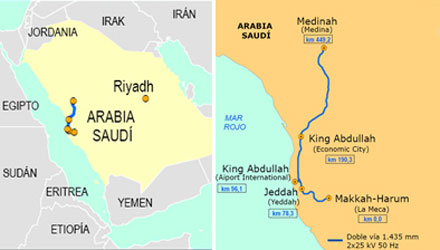
\includegraphics[width=3.66556in,height=2.08252in]{out-img12.png} \par}

{\centering\bfseries
Figure\ 8. High Speed line Medina -- La Meca in Saudi Arabia. Image from
ADIF\ http://international.adif.es/noticias/espana-construira-y-explotara-la-alta-velocidad-entre-medina-y-la-meca-en-arabia-saudi/12/2011/158
\par}


\bigskip

Remote sensing technologies can be applied to assess the risk of
affection in the infrastructure and to minimize and prevent the impact:
Sand movement and speed, risk maps, sand storms monitoring, floods
monitoring, etc.


\bigskip

Satellite imagery can be combined with unmanned aerial vehicles (UAV),
with higher resolution and flexible operation modes, to provide data to
assist in the deployment, operation and maintenance of these lines.\ 

\paragraph[Response]{\selectlanguage{english} Response}

\bigskip

{\selectlanguage{english}
The\ solicited\ service\ is based on the following premises:}

\liststyleLFOvii
\begin{itemize}
\item {\selectlanguage{english}
Coverage during operation of the infrastructure.}
\item {\selectlanguage{english}
Use of archive images to provide information about dunes movements and
speed.}
\item {\selectlanguage{english}
Monthly revisit time.}
\item {\selectlanguage{english}
Urgent images only in case of storms and floods to inspect damages in
the infrastructures.}
\item {\selectlanguage{english}
The images require an analysis to identify risks zones, dune and sand
speed fields, etc.}
\end{itemize}
\paragraph[Data distribution]{\selectlanguage{english} Data
distribution}
\liststyleLFOxiv
\begin{itemize}
\item WMS: A Web Map Service will be deployed to distribute the scenes
of the area of interest to the managers of the infrastructure. Imagery
and derived products (risk maps, wind speed fields, etc.).\ 
\item Value added services (WFS, HTTP/REST, Tiles, etc.). Interactive
value-added services may be provided to the managers in order to have
monitoring tools.\ 
\end{itemize}
\paragraph[Area of Interest]{\selectlanguage{english} Area of Interest}
{\selectlanguage{english}
Several areas of interest have been detected: The Medina -- La Meca
(Saudi Arabia) railway line currently in construction and the south of
Spain (Andaluc\'ia) where testing technologies with sensors and UAV are
in development.}

\paragraph[Users]{\selectlanguage{english} Users}
\liststyleLFOxiii
\begin{itemize}
\item Private organizations, responsible of the construction and
operation of the lines.
\item Public institutions responsible of the management of the railway
infrastructures.
\end{itemize}
\paragraph[Service Type]{\selectlanguage{english} Service Type}
{\selectlanguage{english}
The service type is advanced. It includes mosaics of the area of
interest and combination with other sources of information.}

\paragraph[Processing Level]{\selectlanguage{english} Processing Level}
{\selectlanguage{english}
The processing level is high}

\paragraph[Storage Level]{\selectlanguage{english} Storage Level}
{\selectlanguage{english}
The storage level is high.}

\paragraph[Communications Level]{\selectlanguage{english} Communications
Level}
{\selectlanguage{english}
The communication level is not urgent.}

\paragraph[Demand Variability]{\selectlanguage{english} Demand
Variability}
\foreignlanguage{english}{The demand is variable. See\ }Table
11\foreignlanguage{english}{\ for a summary of the service
characteristics.}

\clearpage
\bigskip

{\centering\bfseries
\label{bkm:Ref377548086}Table\ 11.\ Relation of the users demand with
the service offered in the Scenario 2. In orange the characteristics of
the service.
\par}

\begin{center}
\tablehead{}
\begin{supertabular}{m{0.53165984in}m{0.92955977in}m{0.68855983in}|m{1.0649599in}m{1.1274599in}|m{0.6718598in}m{0.21425986in}}
\hhline{~-----~}
\multicolumn{1}{m{0.53165984in}|}{~
} &
\multicolumn{2}{m{1.6968598in}|}{\centering \bfseries\color{black}
Service Type} &
\multicolumn{2}{m{2.27116in}|}{\centering \bfseries\color{black} Loads
in Cloud Technology} &
\multicolumn{1}{m{0.6718598in}|}{\bfseries\color{black} Demand
Variability} &
~
\\\hline
\multicolumn{1}{|m{0.53165984in}|}{\centering \bfseries\color{black}
COMPANY{\textquotesingle}S SERVICES} &
\multicolumn{1}{m{0.92955977in}|}{\centering \color{black} Basic} &
\centering \color{black} Basic &
\multicolumn{1}{m{1.0649599in}|}{\centering \color{black} Processing} &
\centering \color{black} Low &
\multicolumn{1}{m{0.6718598in}|}{\centering \color{black} Constant} &
\multicolumn{1}{m{0.21425986in}|}{\centering\arraybslash
\textbf{\textcolor{black}{USERS{\textquotesingle}
DE}}\foreignlanguage{spanish}{\textbf{\textcolor{black}{MAND}}}}\\\hline
 &
 &
 &
 &
\centering \selectlanguage{spanish}\color{black} Medium &
 &
\\\hhline{~~~~-~~}
 &
 &
\centering \selectlanguage{spanish}\color{black} Advanced &
 &
\centering \selectlanguage{spanish}\color{black} High &
 &
\\\hhline{~~-~-~~}
 &
 &
 &
\multicolumn{1}{m{1.0649599in}|}{\centering
\selectlanguage{spanish}\color{black} Storage} &
\centering \selectlanguage{spanish}\color{black} Low &
\multicolumn{1}{m{0.6718598in}|}{\centering
\selectlanguage{spanish}\color{black} Variable} &
\\\hhline{~~~---~}
 &
\multicolumn{1}{m{0.92955977in}|}{\centering
\selectlanguage{spanish}\color{black} High added value} &
\centering \selectlanguage{spanish}\color{black} Pull\  &
 &
\centering \selectlanguage{spanish}\color{black} Medium &
 &
\\\hhline{~~-~-~~}
 &
 &
 &
 &
\centering \selectlanguage{spanish}\color{black} High &
 &
\\\hhline{~~~~-~~}
 &
 &
\centering \selectlanguage{spanish}\color{black} Push\  &
\multicolumn{1}{m{1.0649599in}|}{\centering
\selectlanguage{spanish}\color{black} Communications} &
\centering \selectlanguage{spanish}\color{black} Not urgent &
\multicolumn{1}{m{0.6718598in}|}{\centering
\selectlanguage{spanish}\color{black} Highly variable} &
\\\hhline{~~~---~}
 &
 &
 &
 &
\centering \selectlanguage{spanish}\color{black} Urgent &
 &
\\\hhline{~--~-~~}
 &
\multicolumn{2}{m{1.6968598in}|}{\centering
\selectlanguage{spanish}\color{black} Hosting} &
 &
 &
 &
\\\hhline{~--~~~~}
\end{supertabular}
\end{center}

\bigskip

\clearpage
\bigskip

\subsubsection[Scenario 3:\ Land Management {}-- South West of
England]{Scenario 3:\ Land Management -- South West of England}
\hypertarget{Toc381777196}{}\paragraph[Scenario description]{Scenario
description}
\foreignlanguage{english}{There is a need to characterize landscape and
crops in the South West of England, United Kingdom. Besides, the users
demand a multitemporal product which allows analysing the land cover
dynamics and detecting changes.\ }\foreignlanguage{english}{For this
task, multitemporal classification and regression techniques are used
to provide products exploiting the high revisit time, high spatial
resolution}\foreignlanguage{english}{, high swath and
large}\foreignlanguage{english}{\ number of
bands\ }\foreignlanguage{english}{in}\foreignlanguage{english}{\ }\foreignlanguage{english}{the
system\ }(Sensyf)\foreignlanguage{english}{.}

\paragraph[Response]{\selectlanguage{english} Response}
The primary focus of the service is Landscape Management linked to the
use of the land for agricultural purposes versus conservation.\ 


\bigskip

The service is the following:


\bigskip

\liststyleLFOvi
\begin{itemize}
\item Satellite images with a\ weekly\ frequency shall be offered,
including the requested processing through a\ push\ type service.
\item \foreignlanguage{english}{Multitemporal Land Cover Classification
and Change Detection Service are needed. Land cover and land cover
change products will be generated from mosaics with the same temporal
frequency, weekly, and service type, push.}
\end{itemize}
\paragraph[Data distribution]{\selectlanguage{english} Data
distribution}
\liststyleLFOxv
\begin{itemize}
\item WFS to provide direct access to the derived products: Land cover,
etc.
\item Value-added services (REST/HTTP, WMS, Tiles) for the creation of
web applications and interactive solutions.\ 
\end{itemize}
\paragraph[Area of Interest\ ]{\selectlanguage{english} Area of
Interest\ }
\foreignlanguage{english}{The Area of Interest is the\ }South West of
England, United Kingdom, see\ Figure 9.


\bigskip

{\centering   [Warning: Image ignored]
% Unhandled or unsupported graphics:
%\includegraphics[width=2.97361in,height=3.17361in]{out-img13.gif}
 \par}

{\centering\bfseries
\label{bkm:Ref377547646}Figure\ 9.\ South West of England (image
from\ http://www.holiday-home-dealers.co.uk/)
\par}

\paragraph[Users]{\selectlanguage{english} Users}
The user of this service is the European Landscape Convention.

\paragraph[Service Type]{\selectlanguage{english} Service Type}
{\selectlanguage{english}
The service type is high added value (Push). Processing is required to
offer the requested services: crops characterization, classification,
irrigation planning, and change detection.}

\paragraph[Processing Level]{\selectlanguage{english} Processing Level}
{\selectlanguage{english}
The processing level is medium.}

\paragraph[Storage Level]{\selectlanguage{english} Storage Level}
{\selectlanguage{english}
The storage level is medium.}

\paragraph[Communications Level]{\selectlanguage{english} Communications
Level}
{\selectlanguage{english}
The communication level is not urgent since the changes in the crops are
not immediate and the frequency of the images acquisition is higher
than such changes.\ }

\paragraph[Demand Variability]{\selectlanguage{english} Demand
Variability}
The demand is variable.\ It depends on the
season.\ \foreignlanguage{english}{See\ }Table
12\foreignlanguage{english}{\ for a summary of the service
characteristics.}


\bigskip

\clearpage{\centering\bfseries
Table\ 12.\ Relation of the users demand with the service offered in the
Scenario 3. In orange the characteristics of the service.
\par}

\begin{center}
\tablehead{}
\begin{supertabular}{m{0.22605985in}m{0.92955977in}m{0.68855983in}|m{1.0649599in}m{1.1274599in}|m{0.6718598in}m{0.21425986in}}
\hhline{~-----~}
\multicolumn{1}{m{0.22605985in}|}{~
} &
\multicolumn{2}{m{1.6968598in}|}{\centering \bfseries\color{black}
Service Type} &
\multicolumn{2}{m{2.27116in}|}{\centering \bfseries\color{black} Loads
in Cloud Technology} &
\multicolumn{1}{m{0.6718598in}|}{\bfseries\color{black} Demand
Variability} &
~
\\\hline
\multicolumn{1}{|m{0.22605985in}|}{\centering \bfseries\color{black}
COMPANY{\textquotesingle}S SERVICES} &
\multicolumn{1}{m{0.92955977in}|}{\centering \color{black} Basic} &
\centering \color{black} Basic &
\multicolumn{1}{m{1.0649599in}|}{\centering \color{black} Processing} &
\centering \color{black} Low &
\multicolumn{1}{m{0.6718598in}|}{\centering \color{black} Constant} &
\multicolumn{1}{m{0.21425986in}|}{\centering\arraybslash
\textbf{\textcolor{black}{USERS{\textquotesingle}
DEMA}}\foreignlanguage{spanish}{\textbf{\textcolor{black}{ND}}}}\\\hline
 &
 &
 &
 &
\centering \selectlanguage{spanish}\color{black} Medium &
 &
\\\hhline{~~~~-~~}
 &
 &
\centering \selectlanguage{spanish}\color{black} Advanced &
 &
\centering \selectlanguage{spanish}\color{black} High &
 &
\\\hhline{~~-~-~~}
 &
 &
 &
\multicolumn{1}{m{1.0649599in}|}{\centering
\selectlanguage{spanish}\color{black} Storage} &
\centering \selectlanguage{spanish}\color{black} Low &
\multicolumn{1}{m{0.6718598in}|}{\centering
\selectlanguage{spanish}\color{black} Variable} &
\\\hhline{~~~---~}
 &
\multicolumn{1}{m{0.92955977in}|}{\centering
\selectlanguage{spanish}\color{black} High added value} &
\centering \selectlanguage{spanish}\color{black} Pull\  &
 &
\centering \selectlanguage{spanish}\color{black} Medium &
 &
\\\hhline{~~-~-~~}
 &
 &
 &
 &
\centering \selectlanguage{spanish}\color{black} High &
 &
\\\hhline{~~~~-~~}
 &
 &
\centering \selectlanguage{spanish}\color{black} Push\  &
\multicolumn{1}{m{1.0649599in}|}{\centering
\selectlanguage{spanish}\color{black} Communications} &
\centering \selectlanguage{spanish}\color{black} Not urgent &
\multicolumn{1}{m{0.6718598in}|}{\centering
\selectlanguage{spanish}\color{black} Highly variable} &
\\\hhline{~~~---~}
 &
 &
 &
 &
\centering \selectlanguage{spanish}\color{black} Urgent &
 &
\\\hhline{~--~-~~}
 &
\multicolumn{2}{m{1.6968598in}|}{\centering
\selectlanguage{spanish}\color{black} Hosting} &
 &
 &
 &
\\\hhline{~--~~~~}
\end{supertabular}
\end{center}

\bigskip


\bigskip


\bigskip

\clearpage
\bigskip

\subsubsection[Scenario 4: Precision Agriculture {}- Argentina]{Scenario
4: Precision Agriculture - Argentina}
\hypertarget{Toc381777197}{}\paragraph[Scenario description]{Scenario
description}
{\selectlanguage{english}
Small farm operators, cooperatives, large agro-holdings, agricultural
land investment trusts, logistics and supply chain operators need
homogeneous and reliable means to manage\ their\ crops.\ Precision
Agriculture\ provides\ support services for irrigation, based on the
use of Earth Observation (EO) data, hydrological models and
meteorological data.\ Using high resolution imagery, inadequate
irrigation or practices can be identified quickly\ and other
agricultural treatments can be more accurately assessed and optimized.}


\bigskip

\foreignlanguage{english}{In Latin America the leading country is
Argentina, where it was introduced in the middle 1990s with the support
of the National Agricultural Technology
Institute}\foreignlanguage{english}{\ }(Sensyf)\foreignlanguage{english}{,\ }(Astrium)\foreignlanguage{english}{.}

\paragraph[Response]{\selectlanguage{english} Response}
The\ designed constellation will provide\ mosaics of Argentina\ in
a\ daily\ basis, which shall be processed in order to offer several
layers of precise information at the resolution of the satellite system
to the users.

Some processing shall offer info about irrigation planning, improved
management of fertilizer usage, meteorological data affecting crops and
fruit maturity.

\paragraph[Data distribution]{\selectlanguage{english} Data
distribution}
\liststyleLFOxv
\begin{itemize}
\item WFS to provide direct access to the derived products.
\item Value-added services (REST/HTTP, WMS, Tiles) for the creation of
web applications and interactive solutions.\ 
\end{itemize}
\paragraph[Area of Interest\ ]{\selectlanguage{english} Area of
Interest\ }
\foreignlanguage{english}{The Area of Interest is Argentina,
see\ }Figure 10\foreignlanguage{english}{.}


\bigskip

{\centering   [Warning: Image ignored]
% Unhandled or unsupported graphics:
%\includegraphics[width=2.45951in,height=2.64342in]{out-img14.gif}
 \par}

{\centering\bfseries
\label{bkm:Ref377562868}Figure\ 10.\ Map of Argentina
(from\ \url{http://www.dk.co.uk/static/cs/uk/11/worldfactfile/countries/ar.html}).
\par}


\bigskip

\paragraph[Users]{\selectlanguage{english} Users}
{\selectlanguage{english}
The user is the\ National Agricultural Technology Institute.}

\paragraph[Service Type]{\selectlanguage{english} Service Type}
\foreignlanguage{english}{The service type is high added value
(push/hosting) (subscription services for agriculture treatments,
irrigation planning and general monitoring{\dots} Hosting could be
employed for users that do not have where storage the
data)}\foreignlanguage{english}{.}

\paragraph[Processing Level]{\selectlanguage{english} Processing Level}
{\selectlanguage{english}
The processing level is high (several layers of post processing shall be
offered to the users employing mosaics of the country, i.e. the
National Agricultural Technology Institute).}

\paragraph[Storage Level]{\selectlanguage{english} Storage Level}
{\selectlanguage{english}
The storage level is high.\ }

\paragraph[Communications Level]{\selectlanguage{english} Communications
Level}
{\selectlanguage{english}
The communication level is not urgent.}

\paragraph[Demand Variability]{\selectlanguage{english} Demand
Variability}
\foreignlanguage{english}{The demand variability is constant (depending
on the season). See\ }Table 13\foreignlanguage{english}{\ for a summary
of the service characteristics.}


\bigskip


\bigskip

\clearpage{\centering\bfseries
Table\ 13.\ Relation of the users demand with the service offered in the
Scenario 4. In orange the characteristics of the service.
\par}

\begin{center}
\tablehead{}
\begin{supertabular}{m{0.22605985in}m{0.92955977in}m{0.68855983in}|m{1.0649599in}m{1.1274599in}|m{0.6718598in}m{0.21425986in}}
\hhline{~-----~}
\multicolumn{1}{m{0.22605985in}|}{~
} &
\multicolumn{2}{m{1.6968598in}|}{\centering \bfseries\color{black}
Service Type} &
\multicolumn{2}{m{2.27116in}|}{\centering \bfseries\color{black} Loads
in Cloud Technology} &
\multicolumn{1}{m{0.6718598in}|}{\bfseries\color{black} Demand
Variability} &
~
\\\hline
\multicolumn{1}{|m{0.22605985in}|}{\centering \bfseries\color{black}
COMPANY{\textquotesingle}S SERVICES} &
\multicolumn{1}{m{0.92955977in}|}{\centering \color{black} Basic} &
\centering \color{black} Basic &
\multicolumn{1}{m{1.0649599in}|}{\centering \color{black} Processing} &
\centering \color{black} Low &
\multicolumn{1}{m{0.6718598in}|}{\centering \color{black} Constant} &
\multicolumn{1}{m{0.21425986in}|}{\centering\arraybslash
\textbf{\textcolor{black}{USERS{\textquotesingle}
DEM}}\foreignlanguage{spanish}{\textbf{\textcolor{black}{AND}}}}\\\hline
 &
 &
 &
 &
\centering \selectlanguage{spanish}\color{black} Medium &
 &
\\\hhline{~~~~-~~}
 &
 &
\centering \selectlanguage{spanish}\color{black} Advanced &
 &
\centering \selectlanguage{spanish}\color{black} High &
 &
\\\hhline{~~-~-~~}
 &
 &
 &
\multicolumn{1}{m{1.0649599in}|}{\centering
\selectlanguage{spanish}\color{black} Storage} &
\centering \selectlanguage{spanish}\color{black} Low &
\multicolumn{1}{m{0.6718598in}|}{\centering
\selectlanguage{spanish}\color{black} Variable} &
\\\hhline{~~~---~}
 &
\multicolumn{1}{m{0.92955977in}|}{\centering
\selectlanguage{spanish}\color{black} High added value} &
\centering \selectlanguage{spanish}\color{black} Pull\  &
 &
\centering \selectlanguage{spanish}\color{black} Medium &
 &
\\\hhline{~~-~-~~}
 &
 &
 &
 &
\centering \selectlanguage{spanish}\color{black} High &
 &
\\\hhline{~~~~-~~}
 &
 &
\centering \selectlanguage{spanish}\color{black} Push\  &
\multicolumn{1}{m{1.0649599in}|}{\centering
\selectlanguage{spanish}\color{black} Communications} &
\centering \selectlanguage{spanish}\color{black} Not urgent &
\multicolumn{1}{m{0.6718598in}|}{\centering
\selectlanguage{spanish}\color{black} Highly variable} &
\\\hhline{~~~---~}
 &
 &
 &
 &
\centering {\selectlanguage{spanish}\color{black} Urgent}\par

~
 &
 &
\\\hhline{~--~-~~}
 &
\multicolumn{2}{m{1.6968598in}|}{\centering
\selectlanguage{spanish}\color{black} Hosting} &
 &
 &
 &
\\\hhline{~--~~~~}
\end{supertabular}
\end{center}

\bigskip

\clearpage
\bigskip

\subsubsection[Scenario 5: Basemaps {}-- Worldwide]{Scenario 5: Basemaps
-- Worldwide}
\hypertarget{Toc381777198}{}\paragraph[Scenario description]{Scenario
description}
Satellite operators, space agencies and mapping companies offer basemaps
as part of their services and data product. Built from the satellite
scenes, they\ provide seamless and cloud-free coverage of certain
region\ surface\ (countries, continents and worldwide) with multiple
zoom layers and high detail. They are distributed as data archives
(FTP, direct download) or through OGC Web Services (WMS) and Tiles.
These are some examples:


\bigskip

\liststyleLFOxvi
\begin{itemize}
\item NASA{\textquoteright}s Blue\ Marble: offers a
year{\textquoteright}s worth of monthly composites at a spatial
resolution of 500 meters. These monthly images reveal seasonal changes
to the land surface: the green-up and dying-back of vegetation in
temperate regions such as North America and Europe, dry and wet seasons
in the tropics and advancing and retreating Northern Hemisphere snow
cover. They are available for download as georreferenced raster
files.\ 
\end{itemize}

\bigskip

{\centering 
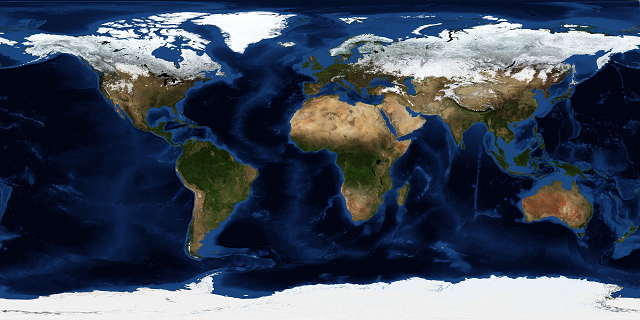
\includegraphics[width=4.65436in,height=2.32718in]{out-img15.png} \par}

{\centering\bfseries
Figure\ 11. NASA{\textquoteright}s Blue Marble from December with
topography and bathymetry.
\par}

\liststyleLFOxvi
\begin{itemize}
\item SPOTMaps: From Astrium, provides 2.5m, natural color, seamless
ortho-mosaics derived from SPOT 5 data, providing nationwide and
regional basemaps for a large part of the globe. They are currently
available over more than 110 countries, and more than 94 million
km{\texttwosuperior}. The coverage is growing and updated on a monthly
basis.
\end{itemize}
\paragraph[Response]{\selectlanguage{english} Response}
With the global daily coverage of the GEO-Cloud constellation of
satellites, a monthly true-color basemap can be built with very high
detail and coverage percentage (cloud-free). In tropical lowlands,
cloud cover during the rainy season can be so extensive that obtaining
a cloud-free view of every pixel of the area for a given month may not
be possible.


\bigskip

Processing will consist of creating monthly mosaics from the daily
coverage of the constellation, removing clouds and applying color
adjustments to create true-color and visually attractive aerial
basemaps.


\bigskip

Resolution of the basemaps will depend on the storage and processing
capacity, it will be studied further during the implementation of the
scenario.

\paragraph[Data distribution]{\selectlanguage{english} Data
distribution}
{\selectlanguage{english}
Data will be delivered though cached WMS and tiles.}

\paragraph[Area of Interest\ ]{\selectlanguage{english} Area of
Interest\ }
{\selectlanguage{english}
The area of interest is the whole world. Country or continent coverages
can be represented. We will focus on Europe.}

\paragraph[Users]{\selectlanguage{english} Users}
\liststyleLFOxvi
\begin{itemize}
\item {\selectlanguage{english}
Governmental clients.}
\item {\selectlanguage{english}
Infrastructure managers.}
\item {\selectlanguage{english}
Third-party service providers.}
\end{itemize}
\paragraph[Service Type]{\selectlanguage{english} Service Type}
{\selectlanguage{english}
The service type is high added value (push/hosting), using on-line
delivery mechanisms.}

\paragraph[Processing Level]{\selectlanguage{english} Processing Level}
{\selectlanguage{english}
The processing level is high (creation of a monthly mosaic from a
catalogue of daily images, cloud removal, color\ adjustments{\dots})}

\paragraph[Storage Level]{\selectlanguage{english} Storage Level}
{\selectlanguage{english}
The storage level is very high. It can be modulated with the maximum
zoom level / resolution offered and the area of interest.}

\paragraph[Communications Level]{\selectlanguage{english} Communications
Level}
{\selectlanguage{english}
The communication level is not urgent.}

\paragraph[Demand Variability]{\selectlanguage{english} Demand
Variability}
\foreignlanguage{english}{The demand variability is variable.
See\ }Table 14\foreignlanguage{english}{\ for a summary of the service
characteristics.}

\clearpage
\bigskip

{\centering\bfseries
\label{bkm:Ref377564650}Table\ 14.\ Relation of the users demand with
the service offered in the Scenario 5. In orange the characteristics of
the service.
\par}

\begin{center}
\tablehead{}
\begin{supertabular}{m{0.22605985in}m{0.92955977in}m{0.68855983in}|m{1.0649599in}m{1.1274599in}|m{0.6718598in}m{0.21425986in}}
\hhline{~-----~}
\multicolumn{1}{m{0.22605985in}|}{~
} &
\multicolumn{2}{m{1.6968598in}|}{\bfseries\color{black} Service Type} &
\multicolumn{2}{m{2.27116in}|}{\bfseries\color{black} Loads in Cloud
Technology} &
\multicolumn{1}{m{0.6718598in}|}{\bfseries\color{black} Demand
Variability} &
~
\\\hline
\multicolumn{1}{|m{0.22605985in}|}{\centering \bfseries\color{black}
COMPANY{\textquotesingle}S SERVICES} &
\multicolumn{1}{m{0.92955977in}|}{\centering \color{black} Basic} &
\centering \color{black} Basic &
\multicolumn{1}{m{1.0649599in}|}{\centering \color{black} Processing} &
\centering \color{black} Low &
\multicolumn{1}{m{0.6718598in}|}{\centering \color{black} Constant} &
\multicolumn{1}{m{0.21425986in}|}{\centering\arraybslash
\textbf{\textcolor{black}{USERS{\textquotesingle}
DEMA}}\foreignlanguage{spanish}{\textbf{\textcolor{black}{ND}}}}\\\hline
 &
 &
 &
 &
\centering \selectlanguage{spanish}\color{black} Medium &
 &
\\\hhline{~~~~-~~}
 &
 &
\centering \selectlanguage{spanish}\color{black} Advanced &
 &
\centering \selectlanguage{spanish}\color{black} High &
 &
\\\hhline{~~-~-~~}
 &
 &
 &
\multicolumn{1}{m{1.0649599in}|}{\centering
\selectlanguage{spanish}\color{black} Storage} &
\centering \selectlanguage{spanish}\color{black} Low &
\multicolumn{1}{m{0.6718598in}|}{\centering
\selectlanguage{spanish}\color{black} Variable} &
\\\hhline{~~~---~}
 &
\multicolumn{1}{m{0.92955977in}|}{\centering
\selectlanguage{spanish}\color{black} High added value} &
\centering \selectlanguage{spanish}\color{black} Pull\  &
 &
\centering \selectlanguage{spanish}\color{black} Medium &
 &
\\\hhline{~~-~-~~}
 &
 &
 &
 &
\centering \selectlanguage{spanish}\color{black} High &
 &
\\\hhline{~~~~-~~}
 &
 &
\centering \selectlanguage{spanish}\color{black} Push\  &
\multicolumn{1}{m{1.0649599in}|}{\centering
\selectlanguage{spanish}\color{black} Communications} &
\centering \selectlanguage{spanish}\color{black} Not Urgent &
\multicolumn{1}{m{0.6718598in}|}{\centering
\selectlanguage{spanish}\color{black} Highly variable} &
\\\hhline{~~~---~}
 &
 &
 &
 &
\centering \selectlanguage{spanish}\color{black} Urgent &
 &
\\\hhline{~--~-~~}
 &
\multicolumn{2}{m{1.6968598in}|}{\centering
\selectlanguage{spanish}\color{black} Hosting} &
 &
 &
 &
\\\hhline{~--~~~~}
\end{supertabular}
\end{center}

\bigskip

\clearpage
\bigskip

\subsubsection[Scenario 6:\ Online Catalogue / Ordering {}--
Worldwide.\ ]{Scenario 6:\ Online Catalogue / Ordering -- Worldwide.\ }
\hypertarget{Toc381777199}{}\paragraph[Scenario description]{Scenario
description}
Having an online browsing, querying and ordering tool for satellites
missions is one of the main elements to request images from the
historic archive.\ 

This kind of tools gives access to the mission archive, discovery tool
gives customers:

\liststyleLFOxvii
\begin{itemize}
\item Access to the mission images archives via the Internet
\item An instant preview of browse images over an area.
\item Searching on metadata.
\item Ability to upload KML, KMZ or shapefiles to refine your area of
interest
\end{itemize}
{\centering 
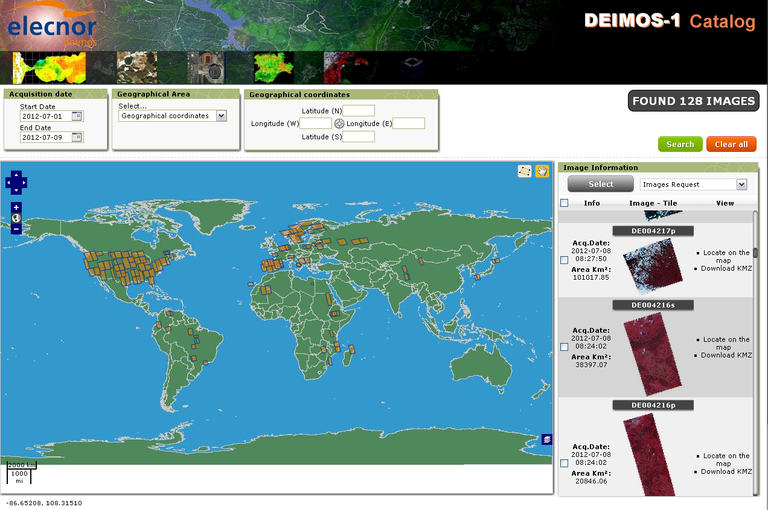
\includegraphics[width=4.46297in,height=2.96407in]{out-img16.png} \par}

{\centering\bfseries
Figure\ 12. DEIMOS-1 Online Catalogue.
\par}

\paragraph[Response]{\selectlanguage{english} Response}
In this scenario, an online catalogue for the constellation of
satellites proposed will be tested, taking into consideration the loads
of users, queries to the catalogue (using CSW standard) and rendering
times for the features (footprints, previews, etc).

\paragraph[Data distribution]{\selectlanguage{english} Data
distribution}
{\selectlanguage{english}
This is a value added service, using CSW to query the catalogue and
HTTP/REST for rendering the previews and footprints.}

\paragraph[Area of Interest\ ]{\selectlanguage{english} Area of
Interest\ }
{\selectlanguage{english}
Worldwide.}

\paragraph[Users]{\selectlanguage{english} Users}
{\selectlanguage{english}
Potential customers/users of the satellite constellation images.}

\paragraph[Service Type]{\selectlanguage{english} Service Type}
{\selectlanguage{english}
Value-added services.}

\paragraph[Processing Level]{\selectlanguage{english} Processing Level}
{\selectlanguage{english}
The processing level is low. Metadata associated with the images is the
main element of processing in this scenario.}

\paragraph[Storage Level]{\selectlanguage{english} Storage Level}
{\selectlanguage{english}
The storage level is high, the images metadata and previews should be
stored.}

\paragraph[Communications Level]{\selectlanguage{english} Communications
Level}
{\selectlanguage{english}
The communication level is not urgent.}

\paragraph[Demand Variability]{\selectlanguage{english} Demand
Variability}
\foreignlanguage{english}{The demand variability is variable.
See\ }Table 15. Relation of the users demand with the service offered
in the Scenario 6. In orange the characteristics of the
service\foreignlanguage{english}{\ for a summary of the service
characteristics.}


\bigskip


\bigskip

\clearpage{\centering\bfseries
Table\ 15.\ Relation of the users demand with the service offered in the
Scenario 6. In orange the characteristics of the service.
\par}

\begin{center}
\tablehead{}
\begin{supertabular}{m{0.22605985in}m{0.92955977in}m{0.68855983in}|m{1.0649599in}m{1.1274599in}|m{0.6718598in}m{0.21425986in}}
\hhline{~-----~}
\multicolumn{1}{m{0.22605985in}|}{~
} &
\multicolumn{2}{m{1.6968598in}|}{\centering \bfseries\color{black}
Service Type} &
\multicolumn{2}{m{2.27116in}|}{\centering \bfseries\color{black} Loads
in Cloud Technology} &
\multicolumn{1}{m{0.6718598in}|}{\bfseries\color{black} Demand
Variability} &
~
\\\hline
\multicolumn{1}{|m{0.22605985in}|}{\centering \bfseries\color{black}
COMPANY{\textquotesingle}S SERVICES} &
\multicolumn{1}{m{0.92955977in}|}{\centering \color{black} Basic} &
\centering \color{black} Basic &
\multicolumn{1}{m{1.0649599in}|}{\centering \color{black} Processing} &
\centering \color{black} Low &
\multicolumn{1}{m{0.6718598in}|}{\centering \color{black} Constant} &
\multicolumn{1}{m{0.21425986in}|}{\centering\arraybslash
\textbf{\textcolor{black}{USERS{\textquotesingle}
DEMA}}\foreignlanguage{spanish}{\textbf{\textcolor{black}{ND}}}}\\\hline
 &
 &
 &
 &
\centering \selectlanguage{spanish}\color{black} Medium &
 &
\\\hhline{~~~~-~~}
 &
 &
\centering \selectlanguage{spanish}\color{black} Advanced &
 &
\centering \selectlanguage{spanish}\color{black} High &
 &
\\\hhline{~~-~-~~}
 &
 &
 &
\multicolumn{1}{m{1.0649599in}|}{\centering
\selectlanguage{spanish}\color{black} Storage} &
\centering \selectlanguage{spanish}\color{black} Low &
\multicolumn{1}{m{0.6718598in}|}{\centering
\selectlanguage{spanish}\color{black} Variable} &
\\\hhline{~~~---~}
 &
\multicolumn{1}{m{0.92955977in}|}{\centering
\selectlanguage{spanish}\color{black} High added value} &
\centering \selectlanguage{spanish}\color{black} Pull\  &
 &
\centering \selectlanguage{spanish}\color{black} Medium &
 &
\\\hhline{~~-~-~~}
 &
 &
 &
 &
\centering \selectlanguage{spanish}\color{black} High &
 &
\\\hhline{~~~~-~~}
 &
 &
\centering \selectlanguage{spanish}\color{black} Push\  &
\multicolumn{1}{m{1.0649599in}|}{\centering
\selectlanguage{spanish}\color{black} Communications} &
\centering
\foreignlanguage{spanish}{\textcolor{black}{Not}}\foreignlanguage{spanish}{\textcolor{black}{\ }}\foreignlanguage{spanish}{\textcolor{black}{urgent}}
&
\multicolumn{1}{m{0.6718598in}|}{\centering
\selectlanguage{spanish}\color{black} Highly variable} &
\\\hhline{~~~---~}
 &
 &
 &
 &
\centering \selectlanguage{spanish}\color{black} Urgent &
 &
\\\hhline{~--~-~~}
 &
\multicolumn{2}{m{1.6968598in}|}{\centering
\selectlanguage{spanish}\color{black} Hosting} &
 &
 &
 &
\\\hhline{~--~~~~}
\end{supertabular}
\end{center}

\bigskip

\clearpage
\bigskip

\subsection[Summary]{Summary}
\hypertarget{Toc381777200}{}
\bigskip

In this\ section\ 6 scenarios has been designed to be tested in the
GEO-Cloud experiment. In addition, the models that will be used to
emulate the end users accessing the BonFIRE cloud have been designed.
From these scenarios and end users models requirements to compute the
processing, storing and distribution of data will be extracted.\ 


\bigskip

Other additional scenarios that might be tested are defined (See
Section\ 9).


\bigskip


\bigskip


\bigskip


\bigskip

\section[Imagery distribution and visualization system design]{Imagery
distribution and visualization system design}
\label{bkm:Ref378924071}\hypertarget{Toc381777201}{}\subsection[Concepts
and evolution of\ imagery distribution and visualization]{Concepts and
evolution of\ imagery distribution and visualization}
\label{bkm:Ref379210422}\hypertarget{Toc381777202}{}The demand and the
requirements for Earth Observation (EO) data\ distribution and
value-added services\ have evolved drastically over the last years. The
amount and the volume of requested data have increased exponentially,
in line with the processing and analyzing capabilities and the number
of EO missions, both private and public, in orbit. In addition, the
variety and the diversity of data requests have increase to a level
where most of the users request and use data from more than one
satellite or satellite operator.

This, in turn, increases the challenge for EO satellite operators, Space
Agencies and EO Data providers to process the data and to offer the
access to the different data as coherently and easily as possible.

EO is a key instrument to the governments (from local to national level)
for the management of critical elements under its umbrella: Natural
resources, climate, economic activities, boundaries control, etc. Thus,
the way this EO information is distributed and managed through
available technologies is focused on interoperability and the
maximization of the investment by reusing the infrastructures.\ 

On the other hand, there is an increasing demand of EO data and services
from new sectors and user typologies, some of which are newcomers to
the EO products. These new users, which are in some cases are
non-experts, are demanding more flexible and instant access to EO
products and services.\ Besides of requiring\ high volume of
data,\ they also demand\ fast and easy access to the data. The
benefit\ from this approach is to reach an increasing number of\ users
and vertical markets.

Both approaches should be considered in an EO\ distribution and
visualization layer, to cover the requirements both from governmental
users, mostly through Spatial Data Infrastructures (SDI)\ and
interoperability standards (OGC) but\ also the general public and
companies outside from the traditional EO workflows.

In the following report, we review the current state of the art for
satellite imagery distribution, visualization and on-line services
creation.

We provide hypothesis on the benefits on using cloud and virtual
infrastructures for EO imagery distribution and the creation of
demand-driven value-added services.

Finally, we propose a high-level architecture for on-line imagery
distribution and services creation to be tested in the Fed4Fire
services.

\subsubsection[Interoperable Earth Observation imagery delivery:
\ Spatial Data Infrastructures]{Interoperable Earth Observation imagery
delivery: \ Spatial Data Infrastructures}
\hypertarget{Toc381777203}{}The term spatial data infrastructure was
coined in 1993 by the U.S. National Research Council to denote a
framework of technologies, policies, and institutional arrangements
that together facilitate the creation, exchange, and use of geospatial
data and related information resources across an information-sharing
community. Such a framework can be implemented narrowly to enable the
sharing of geospatial information within an organization or more
broadly for use at a national, regional, or global level. In all cases,
an SDI will provide an institutionally sanctioned, automated means for
posting, discovering, evaluating, and exchanging geospatial information
by participating\ information producers and users. SDI extends a GIS by
ensuring geospatial data and standards are used to create authoritative
datasets and policies that support it.

Many government administrations have recognized this critical problem
and have initiated coordinated actions to facilitate the discovery and
sharing of spatial data, creating the institutional basis for Spatial
Data Infrastructures (SDI). These efforts were firstly driven in the
90{\textquoteright}s by the U.S with the creation of the Federal
Geographic Data Committee (FGDC). A few years later, Europe joined
these approach by creating ~the European Umbrella Organization for
Geographic Information (EUROGI) and more recently, the Infrastructure
for Spatial Information in Europe (INSPIRE) initiative for the creation
of a European Spatial Data Infrastructure (ESDI). An increasing number
of countries and regions around the world have joined the
implementation of their own SDIs as a\ strategic\ need for their
economic and social development.\ 

SDIs are driven by several standards and initiatives

\liststyleLFOxviii
\begin{itemize}
\item The Open Geospatial Consortium (OGC) Standards.
\item The ISO/TC 211 on\ ISO/TC 211 Geographic information/Geomatics,
responsible for the ISO geographic information series of standards.
\item At European level, INSPIRE and GMES/Copernicus.\ 
\end{itemize}
EO products are relevant for an SDI, since many of the information
managed by these infrastructures come from satellite observations, and
many organizations expect the EO products, even from private missions,
to be delivered through interoperable and standard mechanisms.\ Some of
the standards managed proposed by OGC and ISO are of specific
application to EO data services and data, mainly, in the case of OGC
standards:

\liststyleLFOxix
\begin{itemize}
\item WMS and WMTS: For Web Maps services on Internet.
\item WCS: For accessing coverages data (i.e. raster files from EO
satellites) on Internet.
\item WFS: For accessing features data from\ vector\ data sources on
Internet.
\item CSW: Catalog services on Internet.
\item HMA: HMA provides harmonized and standardized access to ESA
mission data and to other mission ground segments, based on OGC
standards.
\end{itemize}
\subsubsection[Demand{}-driven Earth Observation images
delivery]{Demand-driven Earth Observation images delivery}
\hypertarget{Toc381777204}{}Our modern society is full of spatial
problems that become more and more complex. In order to solve these
complex problems, there is a high demand to high-quality information,
excellent information models, services and software tools, etc.
However, the current Spatial Data Infrastructures (SDIs) are not able
to meet fully these demands (since their developments were more supply
driven). SDIs are built to facilitate the access to data and services.
So far, little attention is given to the actual and desired use of SDIs
for solving spatial problems during the first stages of building SDIs.
Most effort is currently spent to defining data, metadata, standards,
and technology. In other words, the development of the current SDIs is
not based on the needs of the actual, desired and/or potential users.

The complexity of the technologies around the SDIs has caused other
players and technologies to take the place of the SDIs for providing
effective geospatial and EO end-user services. Big companies linked to
the Internet revolution like Google or small specialized companies like
MapBox have redefined, with their own and existing Internet
technologies, the way that geospatial information\ and services are
available via the Internet. Thus, they have driven the universalized
the access to remote sensing and geospatial information beyond
standardization initiatives promoted by the SDIs.

The technologies on top of which these services have been successfully
built are inherited and inspired by the Internet world rather than the
traditional GIS\ industry.\ 

\liststyleLFOxx
\begin{itemize}
\item Cloud and HPC infrastructures to reduce the processing times of
imagery from the satellite and ground stations to an end-user friendly
product.
\item Traditional spatial RDBMS like PostgresSQL and PostGIS, but also
NoSQL databases for handling metadata and other suitable information.
\item Effective delivery mechanisms like CDNs and distributed caches,
mainly based on image tiles.\ 
\item Internet-friendly data interchange formats: Tiles and aggregation
of tiles (MBTiles) for maps and binary imagery and GeoJSON,
TopoJSON\ and UTFGrid\ for features and vectorial information.
\item REST Web Services instead of SOA based, heavy XML interfaces.\ 
\item Client-side processing, leveraging the power of GPUs and user
computers for rendering and analysis: Vector tiles, Canvas, Raster
analysis.
\item Design-driven HTML/JavaScript and Mobile User Interfaces highly
focused on the User Experience.
\end{itemize}
This is how traditional SDI technologies are mapped with these new
technologies.


\bigskip

\begin{flushleft}
\tablehead{}
\begin{supertabular}{|m{3.0260599in}|m{3.2607598in}|}
\hline
\bfseries SDI technology &
\bfseries Demand-driven Geospatial technologies\\\hline
RDBMS and Geoespatial Extensions, Metadata Catalogs. &
RDBMS + NoSQL DB + Geospatial extensions, Metadata Catalogs.\\\hline
Geospatial Application servers (Map servers, features servers &
Tile servers. Rest Web Services.\\\hline
WMS, WMST, Cached Tiles. &
Cached Tiles, MBTiles, CDNs.\\\hline
WFS &
REST WS/GeoJSON, REST WS/TopoJSON\\\hline
WPS &
Cloud processing, REST WS\\\hline
WCS &
REST WS\\\hline
\end{supertabular}
\end{flushleft}

\bigskip

\subsection[Geo{}-Cloud Image Distribution and Visualization System
(Geo{}-Cloud IDV) design]{Geo-Cloud Image Distribution and
Visualization System (Geo-Cloud IDV) design}
\hypertarget{Toc381777205}{}From the geospatial technologies and
standards reviewed in Section\ 4.1, a selection is made to fulfill
several requirements specific to Earth Observation imagery and use
cases and better suite in a distributed infrastructure provided by the
Fed4Fire testbeds.\ 

For interoperability purposes, most distribution mechanisms will be
standards-based (OGC). Some standards, like CSW, are not taken into
consideration since they are not intended for a massive use in the EO
imagery generation workflow.\ 

HMA is not yet currently taken into consideration since it is still and
work in progress standard. More user-focused approaches will be adopted
for value-added products and services, and fast visualization.

For the experiments designed, the focus will be on WMS and Tiles
distribution mechanisms.

\subsubsection[Distribution and Visualization mechanisms for Geo{}-Cloud
IDV]{Distribution and Visualization mechanisms for Geo-Cloud IDV}
\hypertarget{Toc381777206}{}\paragraph[FTP]{FTP}
This will be the mechanism to distribute the raw data from the ground
stations to the distribution infrastructure. Moreover, raw data can be
delivered to the end user by this simple mechanisms using simple access
protocol (user/password, SFTP accounts, etc.). This is the more common
way to distribute the images and products in the industry nowadays.\ 

\paragraph[WMS]{WMS}
A Web Map Service (WMS) enables the visualization of EO data on the
World Wide Web. This standard does not provide the actual raw data;
instead it just provides a georeferenced image (e.g. PNG, JPEG or GIF
files) of the data that can be queried by bounding box, reprojected,
styled, etc. It enables the integration into GIS clients and spatial
data infrastructures.

In the case of large and high resolution EO imagery, the following
workflow is needed in order to provide efficient delivery through WMS:

\liststyleLFOxxi
\setcounter{saveenum}{\value{enumi}}
\begin{enumerate}
\setcounter{enumi}{\value{saveenum}}
\item Image Mosaics. Preparation of Image Mosaics from separate
georeferenced images from the satellites for an area of
interest,\ assembling\ a set of overlapping geospatially rectified
images into a\ continuous\ image. Additionally to preparing the mosaic,
it is convenient\ the\ creation\ of
{\textquotedblleft}overviews{\textquotedblright} within the file, which
is basically a downsampled version of the raster data suitable for use
at lower resolutions.\ 
\end{enumerate}
{\centering 
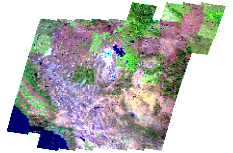
\includegraphics[width=2.08145in,height=1.36709in]{out-img17.png} \par}

{\centering\bfseries
Figure\ 13. Mosaic of images from different satellite scenes.\ 
\par}

\liststyleLFOxxi
\setcounter{saveenum}{\value{enumi}}
\begin{enumerate}
\setcounter{enumi}{\value{saveenum}}
\item Image Pyramids. For very large images, it is convenient to build
Image Pyramids. An image pyramid builds multiple mosaics of images,
each one at a different zoom level, making it so that each tile is
stored in a separate file. This comes with a composition overhead to
bring back the tiles into a single image, but can speed up image
handling through WMS as each overview is tiled, and thus a sub-set of
it can be accessed efficiently (as opposed to a single GeoTIFF, where
the base level can be tiled, but the overviews never are).
\end{enumerate}
{\centering 
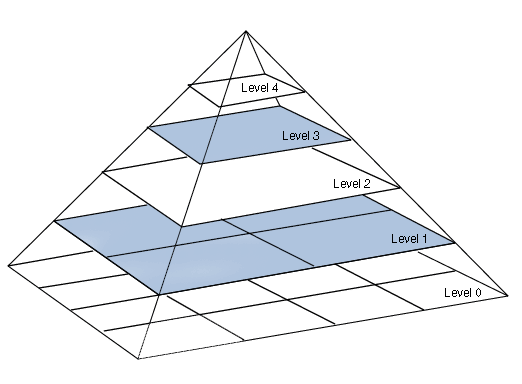
\includegraphics[width=3.27795in,height=2.4151in]{out-img18.png} \par}

{\centering\bfseries
Figure\ 14. Building Image Pyramids.
\par}

Once the mosaics and pyramids are created from the original data
sources, delivery through WMS is more efficient.\ 

The number of pyramids needed depend on the pixels size of the image and
the tile size, and it is given by the following formula:

{\centering\bfseries
\label{bkm:Ref252536537}Equation\ 1. Number of pyramids.
\par}

{\centering \par}

where\ \ is the number of pyramids,\ \ is the image size in pixels,
and\ \ is the tile size in pixels.

For example, for a square area of\ 1.675 km{\texttwosuperior}\ (Lorca
extension, a village in Spain, see\ Section\ 3), an image mosaic built
from satellite scenes with a resolution of 6.7 m/pixel
(see\ Section\ 1) will have a size of 250.000 x 250.000 pixels.
From\ Equation 1\ and for a tile size of 512 x 512 pixels, this gives 8
for the number of pyramids needed.

\paragraph[WFS]{WFS}
Web Feature Service (WFS) defines a standard for exchanging vector data
over the Internet. With compliant WFS, clients can query both the data
structure and the source data. Advanced WFS operations also support
feature locking and edit operations.

\paragraph[WCS]{WCS}
The Web Coverage Service (WCS) supports the networked interchange of
geospatial data as {\textquotedbl}coverages{\textquotedbl} containing
values or properties of geographic locations \ The specification
details interfaces that allow client applications to seamlessly query
and access raw or processed satellite imagery, digital elevation
models, raster data, and other types of coverage data stored on one or
more distributed servers.

Unlike the Web Map Service (WMS) which filters and portrays spatial data
as static geo-registered {\textquotedbl}pictures{\textquotedbl}, the
Web Coverage Service provides allows a client application to query and
access geospatial information that represents a fully tessellated
surface (satellite data, digital orthophotos, and so forth). The
returned data can be used for client-side rendering, multi-valued
coverage analysis, and input into scientific models and other
client\ applications beyond simple viewers.

\paragraph[Web Maps, Tiles and Tiles Caches]{Web Maps, Tiles and Tiles
Caches}
Tiles are the fastest mechanism to visualize EO imagery on the Internet.
They are not intended for direct distribution, and are\ pre-rendered
with certain quality, zoom levels and projections.\ 

A continuous image of the world at street level detail, the kind of
resolution\ managed offered by the constellation proposed,\ would be
millions of pixels wide -- much too large to download or hold in memory
at once using WMS protocols.\ 

In practice, when creating maps for the Web, they are made up of many
small, square images called tiles which are typically 256 x 256 pixels
and are placed side-by-side in order to create the illusion of a very
large seamless image.\ 

The way\ to get more\ detail in maps is\ by using\ zoom levels. Higher
zoom levels increase the physical size of the displayed map but also
increase the amount of detail shown.

{\centering 
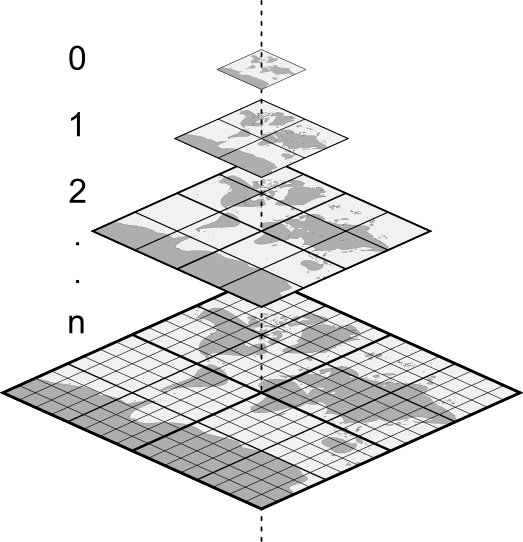
\includegraphics[width=2.46933in,height=2.55614in]{out-img19.png} \par}

{\centering\bfseries
Figure\ 15. Mercator tile pyramid. Each tile is 256 x 256 pixels.
\par}

Google Maps, Microsoft Virtual Earth, Yahoo Maps, and other commercial
API providers as well as OpenStreetMap are using the same projection
and tiling profile and tiles are therefore compatible. The extents of
all tiles as well as the zoom levels (resolution in meters per pixel)
are predefined for the whole Earth. The difference is only in the way
how the equivalent tiles are indexed. There are three main systems of
tile addressing: Google XYZ, Microsoft QuadTree and other OGC or OSGeo
standards or recommendations like TMS, WMTS and WMS-C.

 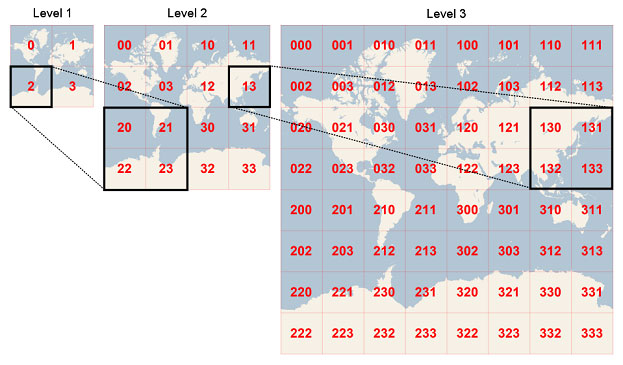
\includegraphics[width=6.29861in,height=3.68976in]{out-img20.jpg} 

{\centering\bfseries
Figure\ 16. Bing Maps tiles scheme.
\par}


\bigskip

To display the tiles, projection has to be also taken into
consideration. For Web Maps based on tiles, Spherical Mercator
EPSG:900913 (EPSG:3857) and WGS84 Datum are commonly used.

When using this projection, the resolution and scale for zoom level at
equator (scales will fluctuate with latitude) can be calculated with
the following formula:

{\centering\bfseries
Equation\ 2. Resolution per zoom level.
\par}

{\centering \par}


\bigskip

The number of tiles for squared projections is\ , where\ \ is the number
of tiles and\ \ the zoom level.

For an average tile size of 20 KB, this gives the following estimation
of resolutions, number of tiles and size on disk per zoom level.\ 

{\centering\bfseries
Table\ 16. Resolution, tiles and size per zoom level.
\par}

\begin{center}
\tablehead{}
\begin{supertabular}{|m{0.7517598in}|m{1.3343599in}|m{1.1149598in}|m{1.1288599in}|}
\hline
\raggedleft Zoom level &
\raggedleft Resolution (m/pixel) &
\raggedleft Number of Tiles &
\raggedleft\arraybslash Size on disk (MB)\\\hline
\raggedleft 1 &
\raggedleft \foreignlanguage{spanish}{78271.52} &
\raggedleft 4 &
\raggedleft\arraybslash 0\\\hline
\raggedleft 2 &
\raggedleft \foreignlanguage{spanish}{39135.76} &
\raggedleft 16 &
\raggedleft\arraybslash 0\\\hline
\raggedleft 3 &
\raggedleft \foreignlanguage{spanish}{19567.88} &
\raggedleft 64 &
\raggedleft\arraybslash 0\\\hline
\raggedleft 4 &
\raggedleft \foreignlanguage{spanish}{9783.94} &
\raggedleft 256 &
\raggedleft\arraybslash 0\\\hline
\raggedleft 5 &
\raggedleft \foreignlanguage{spanish}{4891.97} &
\raggedleft 1,024 &
\raggedleft\arraybslash 0\\\hline
\raggedleft 6 &
\raggedleft \foreignlanguage{spanish}{2445.98} &
\raggedleft 4,096 &
\raggedleft\arraybslash 0\\\hline
\raggedleft 7 &
\raggedleft \foreignlanguage{spanish}{1222.99} &
\raggedleft 16,384 &
\raggedleft\arraybslash 0\\\hline
\raggedleft 8 &
\raggedleft \foreignlanguage{spanish}{611.50} &
\raggedleft 65,536 &
\raggedleft\arraybslash 1\\\hline
\raggedleft 9 &
\raggedleft \foreignlanguage{spanish}{305.75} &
\raggedleft 262,144 &
\raggedleft\arraybslash 5\\\hline
\raggedleft 10 &
\raggedleft \foreignlanguage{spanish}{152.87} &
\raggedleft 1,048,576 &
\raggedleft\arraybslash 20\\\hline
\raggedleft 11 &
\raggedleft \foreignlanguage{spanish}{76.44} &
\raggedleft 4,194,304 &
\raggedleft\arraybslash 80\\\hline
\raggedleft 12 &
\raggedleft \foreignlanguage{spanish}{38.22} &
\raggedleft 16,777,216 &
\raggedleft\arraybslash 320\\\hline
\raggedleft 13 &
\raggedleft \foreignlanguage{spanish}{19.11} &
\raggedleft 67,108,864 &
\raggedleft\arraybslash 1,280\\\hline
\raggedleft 14 &
\raggedleft \foreignlanguage{spanish}{9.55} &
\raggedleft 268,435,456 &
\raggedleft\arraybslash 5,120\\\hline
\raggedleft 15 &
\raggedleft \foreignlanguage{spanish}{4.78} &
\raggedleft 1,073,741,824 &
\raggedleft\arraybslash 20,480\\\hline
\raggedleft 16 &
\raggedleft \foreignlanguage{spanish}{2.39} &
\raggedleft 4,294,967,296 &
\raggedleft\arraybslash 81,920\\\hline
\raggedleft 17 &
\raggedleft \foreignlanguage{spanish}{1.19} &
\raggedleft 17,179,869,184 &
\raggedleft\arraybslash 327,680\\\hline
\raggedleft 18 &
\raggedleft \foreignlanguage{spanish}{0.60} &
\raggedleft 68,719,476,736 &
\raggedleft\arraybslash 1,310,720\\\hline
\raggedleft 19 &
\raggedleft \foreignlanguage{spanish}{0.30} &
\raggedleft 274,877,906,944 &
\raggedleft\arraybslash 5,242,880\\\hline
\end{supertabular}
\end{center}
\subparagraph{Tiles caches}
Web Maps are often static. As most mapping clients render WMS (Web Map
Service) data every time they are queried, this can result in
unnecessary processing and increased wait times. Tile Caches optimizes
this process by saving (caching) map images, or tiles, as they are
requested, in effect acting as a proxy between client and any WMS
server.

As new maps and tiles are requested, the tiles caches intercepts these
calls and returns pre-rendered tiles if stored, or calls the server to
render new tiles as necessary. Thus, once tiles are stored, the speed
of map rendering increases by many times, creating a much improved user
experience.

A tiling strategy controls when your tiles are created and for what
areas (geographic extents) they are created. Tile sets can be created
proactively (by {\textquotedblleft}seeding{\textquotedblright}), or
on-demand.

\textbf{Seeding}\textbf{:\ }Seeding creates tiles prior to requests from
clients, so that they will already be available when the first users
start navigating the map. Because the images exist on the server, there
is never any wait time for the tile to be rendered, and is sent
immediately to the client.

While seeding is very responsive to the end-user, there are some
disadvantages to the administrator:

\liststyleLFOxxii
\begin{itemize}
\item Planning the tile strategy takes time.
\item Creating the tiles takes computing power (typically days for
processing zoom levels {\textgreater} 12 and the time to seed grows
exponentially).
\item Storing the tiles takes disk space.
\end{itemize}
\textbf{On-Demand caching}: Caching tiles
{\textquotedblleft}on-demand{\textquotedblright} mean that the first
user/client to navigate to an uncached area will wait while the
corresponding tiles are drawn by the server, and then delivered to the
client. Once rendered, the tiles are added to the
service{\textquoteright}s cache folder and remain on the server until
updated or deleted by the expiration policy or cache administrator.
Subsequent visitors to that same area will not have to wait for the
tiles to be rendered, because they{\textquoteright}ll already exist.

The main advantage to on-demand caching is that it requires no
preprocessing, and because only the data requested will be cached it
can potentially save disk space. The disadvantage of on-demand caching
is that because viewing will be slower and then intermittently
accelerated it can affect the quality of the user experience.

In practice, a compromise between both strategies has to be accomplished
depending on the use case.

\paragraph[CDN and distributed caching]{CDN and distributed caching}
To speed-up the tiles distribution to the end-users, CDNs and
distributed caching can be used. At the end, tiles are just static
files that can be deployed in several nodes in a CDN and served to the
client,\ optimizing\ the\ performance,\ by selection of node\ locations
that are best for serving content to the user. This may be measured by
choosing locations that are the fewest hops, the least number of
network seconds away from the requesting client, or the highest
availability in terms of server performance (both current and
historical). Examples of CDNs are Akamai or Amazon CloudFront.

{\centering 
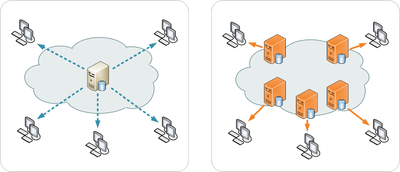
\includegraphics[width=4.16528in,height=1.79097in]{out-img21.png} \par}

{\centering\bfseries
Figure\ 17. CDN architecture.
\par}

\paragraph[Value{}-added products and services]{Value-added products and
services}
Value added products and services typically involve the processing of
the satellite scenes and its bands to produce post-processed products
with additional value beyond the raw data.\ 

These value-added products cover different markets\ and use cases, as
described in Section\ 3:\ hydrology, agriculture, environmental
monitoring, intelligence, urban development and infrastructures
monitoring, mapping, land management (topology, geology, forestry),
disaster monitoring and maritime surveillance, etc.

\begin{flushleft}
\tablehead{}
\begin{supertabular}{c}
 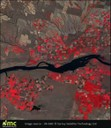
\includegraphics[width=1.15625in,height=1.33056in]{out-img22.jpg} 
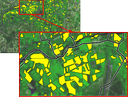
\includegraphics[width=1.33056in,height=1.00903in]{out-img23.png} 
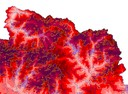
\includegraphics[width=1.33056in,height=0.97361in]{out-img24.jpg} 
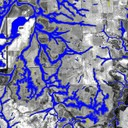
\includegraphics[width=1.33056in,height=1.33056in]{out-img25.jpg} \\
\end{supertabular}
\end{flushleft}
{\centering\bfseries
Figure\ 18. Remote Sensing value-added products.
\par}

Moreover, there is an increasing demand for on-line services based on
those products. These services can be delivered though vertical
solutions and businesses though Internet (web portals and applications)
or by providing APIs and controlled and programmatic access to these
data (APIs and Web Services).\ 

\paragraph[Summary]{Summary}
Depending on the use case and scenario, a distribution and visualization
mechanism should be chosen. In the following table, we present a
summary of the different alternatives evaluated.

\begin{center}
\tablehead{}
\begin{supertabular}{|m{1.2003598in}|m{1.2003598in}|m{1.2003598in}|m{1.2003598in}|}
\hline
~
 &
Pros &
Cons &
When to use\\\hline
FTP &
Simple and direct mechanism &
Only for distribution. Not selection, query, etc. &
Access to RAW data.\\\hline
WMS/WFS/WCS &
Standards based &
Low performance,\ hard to understand for non-experts. &
When the user needs access to\ raw or processed data and features for
certain areas and custom projections, bounding boxes, etc.

Low users demand.\\\hline
Cached Tiles (WMTS{\dots}) &
Fast. Standards-based. &
Pre-rendered. Fixed projections.\  &
Massive user services, value added services.\\\hline
REST/HTTP &
Fast, easy to integrate &
Non-standard (although some OGC services have been extended to REST
interfaces) &
Massive user services, value added services.\\\hline
CDN &
Fast delivery &
Hard to configure and deploy.

Non standard. &
~
\\\hline
\end{supertabular}
\end{center}
\subsubsection[Geo{}-Cloud IDV Architecture]{Geo-Cloud IDV Architecture}
\hypertarget{Toc381777207}{}{\centering 
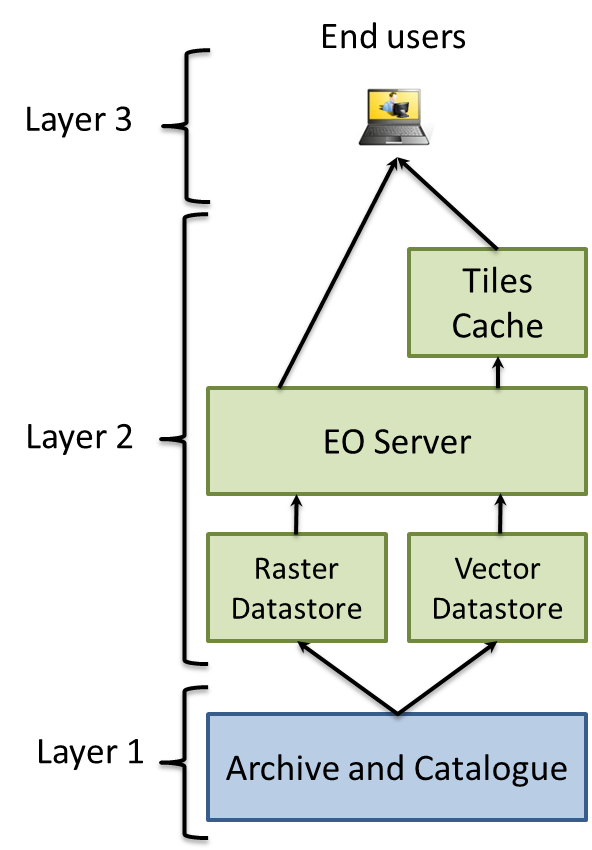
\includegraphics[width=2.11941in,height=3.04301in]{out-img26.png} \par}

{\centering\bfseries
Figure\ 19. Components architecture for data distribution and
visualization.
\par}

\paragraph[Components]{Components}
\subparagraph{Archive and Catalogue}
The processed images will be stored and catalogued for their
distribution in both ways direct downloading (low added value services)
and web based service (high added value services), as described
in\ Section\ 5.

\subparagraph{Datastore}
The datastore will be fed from the archive and catalogue with the
required scenes from the archive to cover the uses cases specified in
TEC-02. In some cases, additional processing will be needed to optimize
these scenes for distribution through OGC Web Services, to populate the
tiles cache, etc.

\begin{center}
\tablehead{}
\begin{supertabular}{|m{1.0010599in}|m{1.5198599in}|m{1.5205599in}|m{1.5205599in}|}
\hline
\centering \bfseries Instance type &
\centering \bfseries CPU cores &
\centering \bfseries Memory &
\centering\arraybslash \bfseries Features\\\hline
\centering storage &
\centering {}- &
\centering \ 300 GB &
~
\\\hline
\end{supertabular}
\end{center}

\bigskip

The datastore will be based on two components:

\liststyleLFOxxiii
\begin{itemize}
\item A geospatial database, to handle geometries and vector features,
and in some cases, raster files. It will be based on PostGIS database.
\item The instance filesystem.
\end{itemize}
\subparagraph{EO Server}
A map and feature server for sharing, analyzing, and editing geospatial
data from spatial data sources using open standards. It implements OGC
Web Services (WMS, WFS, WCS, etc.) as well as providing tiling and
cache mechanisms.\ 

For most of its web services, it can be scaled horizontally by adding
several EO Server nodes to the infrastructure.\ 

\begin{center}
\tablehead{}
\begin{supertabular}{|m{1.0010599in}|m{1.5198599in}|m{1.5205599in}|m{1.5205599in}|}
\hline
\centering \bfseries Instance type &
\centering \bfseries CPU cores &
\centering \bfseries Memory &
\centering\arraybslash \bfseries Features\\\hline
\centering \textrm{\textcolor{black}{xlarge+}} &
\centering 4 &
\centering \ 8GB &
Higher CPU clock speed (over 3GHz)\\\hline
\end{supertabular}
\end{center}

\bigskip

\begin{center}
\tablehead{}
\begin{supertabular}{|m{1.0010599in}|m{1.5198599in}|m{1.5205599in}|m{1.5205599in}|}
\hline
\centering \bfseries Instance type &
\centering \bfseries CPU cores &
\centering \bfseries Memory &
\centering\arraybslash \bfseries Features\\\hline
\centering Load balancer &
\centering {}- &
\centering \ {}- &
\centering\arraybslash EaaS\\\hline
\end{supertabular}
\end{center}

\bigskip

It will be based on the Open Source SW GeoServer.\ 

{\centering 
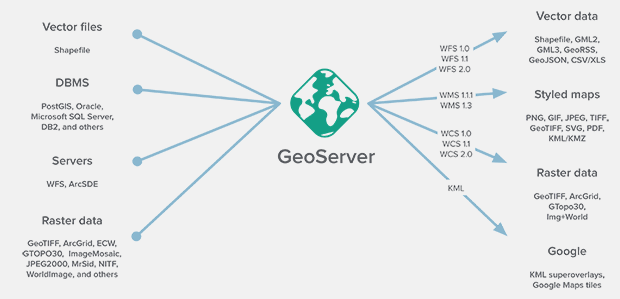
\includegraphics[width=4.87185in,height=2.34743in]{out-img27.png} \par}

{\centering\bfseries
Figure\ 20. Geoserver features.
\par}

\subparagraph{Tiles Caches}
For the tiles cache,\ GeoWebCache\ will be used.\ \ It is\ s a Java web
application used to cache map tiles coming from a variety of sources
such as OGC Web Map Service (WMS). It implements various service
interfaces (such as WMS-C, WMTS, TMS, Google Maps KML, Virtual Earth)
in order to accelerate and optimize map image delivery. It can also
recombine tiles to work with regular WMS clients.

GeoWebCache can scale horizontally by adding nodes sharing the same
cache data store. To store the cached tiles, high storage capacity is
needed.

\begin{center}
\tablehead{}
\begin{supertabular}{|m{1.0010599in}|m{1.5198599in}|m{1.5205599in}|m{1.5205599in}|}
\hline
\centering \bfseries Instance type &
\centering \bfseries CPU cores &
\centering \bfseries Memory &
\centering\arraybslash \bfseries Features\\\hline
\centering storage &
\centering {}- &
\centering \ 500 GB &
~
\\\hline
\end{supertabular}
\end{center}

\bigskip

\begin{center}
\tablehead{}
\begin{supertabular}{|m{1.0010599in}|m{1.5198599in}|m{1.5205599in}|m{1.5205599in}|}
\hline
\centering \bfseries Instance type &
\centering \bfseries CPU cores &
\centering \bfseries Memory &
\centering\arraybslash \bfseries Features\\\hline
\centering Custom &
\centering 4 &
\centering \ 2GB &
Higher CPU clock speed (over 3GHz)\\\hline
\end{supertabular}
\end{center}

\bigskip

\begin{center}
\tablehead{}
\begin{supertabular}{|m{1.0010599in}|m{1.5198599in}|m{1.5205599in}|m{1.5205599in}|}
\hline
\centering \bfseries Instance type &
\centering \bfseries CPU cores &
\centering \bfseries Memory &
\centering\arraybslash \bfseries Features\\\hline
\centering Load balancer &
\centering {}- &
\centering \ {}- &
\centering\arraybslash EaaS\\\hline
\end{supertabular}
\end{center}

\bigskip

\paragraph[Distributed architecture]{Distributed architecture}
{\centering 
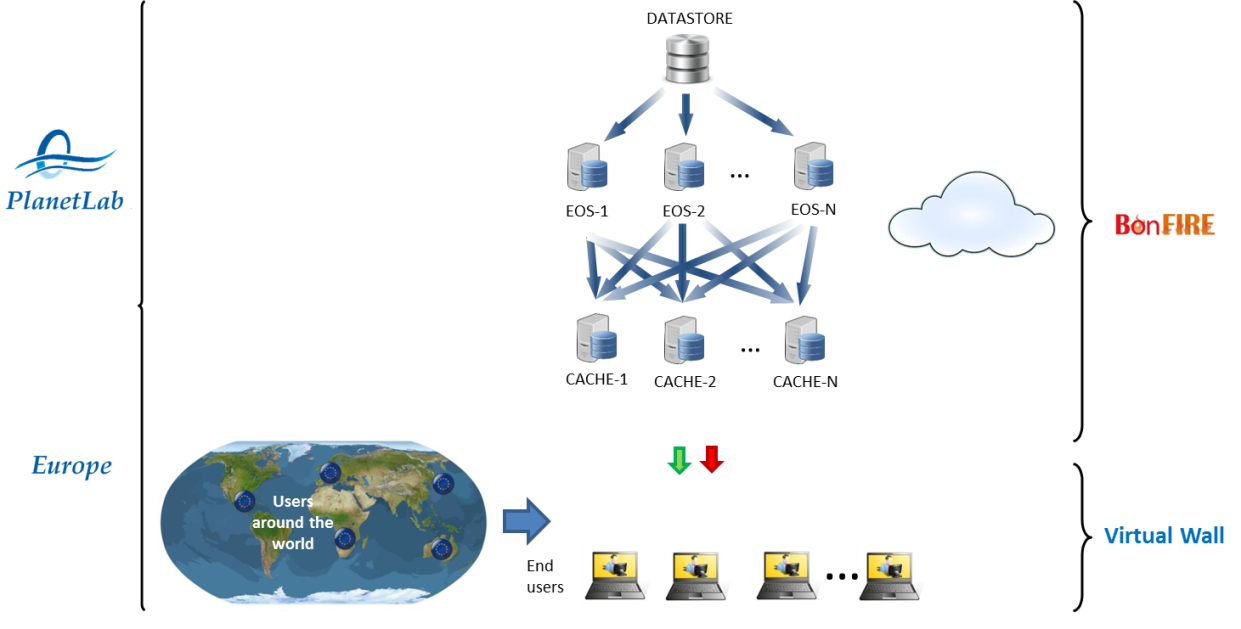
\includegraphics[width=5.63567in,height=2.85821in]{out-img28.png} \par}

{\centering\bfseries
Figure\ 21. Geo-Cloud IDV in Fed4Fire.
\par}

Since some of the components of the GEO-Cloud IDV may scale
horizontally, the EaaS feature of BonFire will be used.

{\centering 
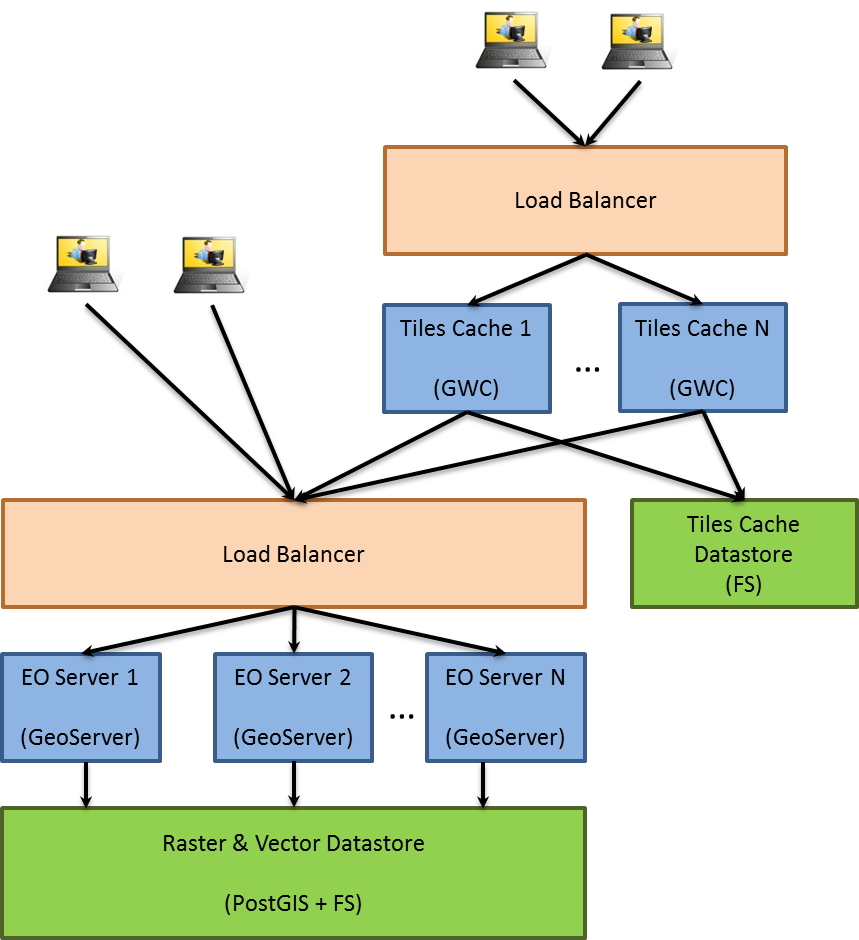
\includegraphics[width=3.31233in,height=3.62481in]{out-img29.png} \par}

{\centering\bfseries
Figure\ 22. GEO-Cloud IDV Instances.
\par}

\subsection[Summary]{Summary}
\hypertarget{Toc381777208}{}We have proposed an initial architecture for
the Imagery Distribution and Visualization System for the GEO-Cloud
experiment (GEO-Cloud IDV). From a selection of distribution and
visualization mechanisms, we have selected the ones that better fit in
the use cases and satellite system designed. Making use of the BonFire
facilities, the objective is to push the system to the limits to test
massive EO data distribution and service delivery using cloud
infrastructures.


\bigskip

\section[Data processing and storage in\ BonFIRE]{Data processing and
storage in\ BonFIRE}
\label{bkm:Ref378929340}\hypertarget{Toc381777209}{}
\bigskip

In this document the data processing chain in to be implemented in the
BonFIRE cloud is presented. This chain begins after the reception of
the images in the ground stations, which are emulated in Virtual Wall.
Thus, direct connection between Virtual Wall and BonFIRE is required.


\bigskip

The whole product processing chain is intended to be implemented in
cloud. For that purpose an orchestrator that manages the processing
stages of the data and the cloud has to be ad hoc implemented during
the implementation stage of the experiment.


\bigskip

For the data delivery and distribution, Web Services (based on OGC
standards and state-of-the-art Web technologies) will be used.\ 


\bigskip

In addition, the data distribution modules will be connected to Virtual
Wall, where VMs with different processing loads emulating end users
accessing the GEO-Cloud services will be implemented.


\bigskip


\bigskip

{\centering 
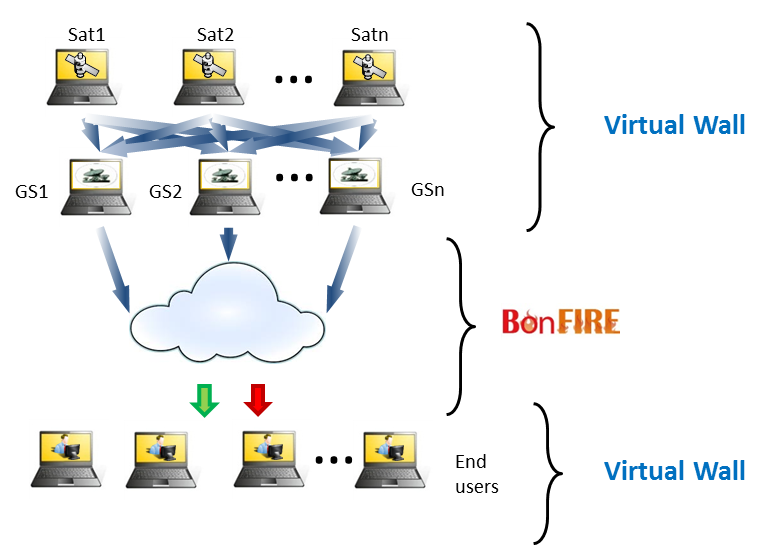
\includegraphics[width=4.24881in,height=3.02652in]{out-img30.png} \par}

{\centering\bfseries
Figure\ 23.\ Relation between BonFIRE and Virtual Wall.
\par}

\subsection[Architecture]{Architecture}
\hypertarget{Toc381777210}{}
\bigskip

The first approach of the architecture to be implemented in the BonFIRE
is constituted of two layers (see\ Figure 24):


\bigskip

\liststyleLFOxxv
\setcounter{saveenum}{\value{enumi}}
\begin{enumerate}
\setcounter{enumi}{\value{saveenum}}
\item \textbf{Layer 1}\textbf{:\ }This layer involves the basic
satellite imagery services. \ It acquires the raw data, has the first
level of processing,\ distributes the processed data, stores the
processed data and\ offers the hosting service. The storage servers
will have three functions: i)\ hosting service for end users,
ii)\ processing of\ the raw data\ and\ required metadata (this data
will be stored in a long term basis) and iii) storage of processed data
for its later distribution.\ During the experiment implementation and
execution we will define at which levels of processing the images will
be stored in cloud. A first approach is to store the raw data and the
L1C images, although this strategy can suffer changes.
\end{enumerate}

\bigskip

\liststyleLFOxxv
\setcounter{saveenum}{\value{enumi}}
\begin{enumerate}
\setcounter{enumi}{\value{saveenum}}
\item \textbf{Layer 2:\ }This layer involves the high added value
services. It can use historical processed data from layer 1. This layer
processes the information for real time generation of geo-information
and offers real time access and distribution to the end-users.
Typically, the implementation of high added value EO services involves
the ingestion of the raster imagery from the satellites into a spatial
database or storage, where it can be refined, simplified, processed or
combined with other data sources in vector or raster format. The
products, which can be themselves vector or raster data, are
distributed or queried using Internet technologies (OGC standards like
WMS, WPS, WCS, CSW, etc. and geo-information servers) or through more
pragmatic and efficient mechanisms: REST Web Services, GeoJSON data
formats, tiles, caches and Content Delivery Networks (CDN).\ 
\end{enumerate}

\bigskip

{\centering 
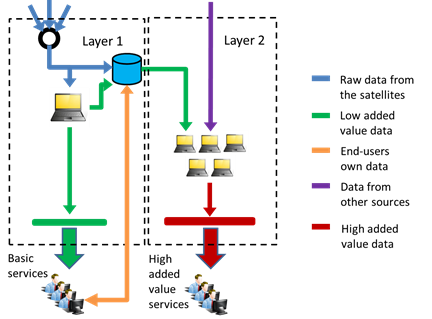
\includegraphics[width=2.88056in,height=2.12708in]{out-img31.png} 
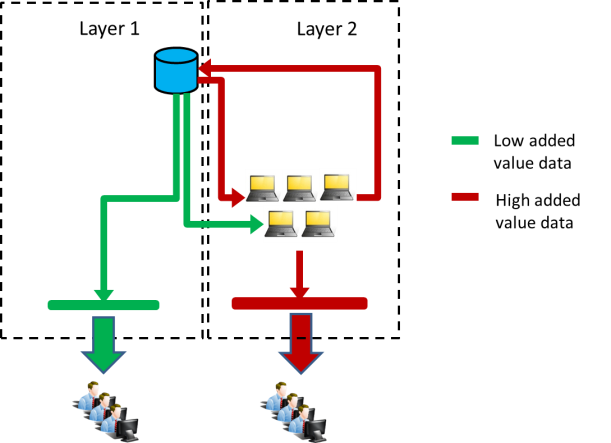
\includegraphics[width=2.77773in,height=2.01522in]{out-img32.png} \par}


\bigskip

{\centering\bfseries
\label{bkm:Ref378172684}Figure\ 24.\ First approach of the architecture
to be implemented in BonFIRE. Two layered EO model in BonFIRE cloud:
Cloud model for storage, processing and distribution (left). Short term
storage of processed information for its later distribution,
postprocessing or both (right).
\par}


\bigskip

The architecture depicted in\ Figure 24\ will be evaluated. Then it can
suffer modifications during the implementation stage in BonFIRE. In
principle this is the strategy:


\bigskip

\liststyleLFOxxxiv
\setcounter{saveenum}{\value{enumi}}
\begin{enumerate}
\setcounter{enumi}{\value{saveenum}}
\item The raw data is received and stored. We will evaluate if it is
better to store raw data or images processed at a low level, such as
L0.
\item The raw data is processed until an orthorectified image is
obtained.
\item The orthorectified image can be directly distributed (we will
analyze if this can be done during the implementation and
experimentation stages) and stored to be used in high added value
services or direct distribution. We will evaluate if the cloud is fast
enough to avoid storage of orthorectified images, and process on demand
raw data or data processed at a\ low level, for example L0. Although
our first impression is that we will have to store all the
orthorectified images for its distribution through high added value
services.
\item Data from other sources will be integrated for its distribution.
\end{enumerate}

\bigskip

The modules that constitute the different layers of the architecture are
depicted in\ Figure 25\ and they are described as follows:


\bigskip

\liststyleLFOxxiv
\begin{itemize}
\item \textbf{Orchestrator:}\ it manages the automatic distribution of
the raw data to the processors. It handles the complete automatic
processing chain execution. \ If the processor chain is occupied, the
manager replicates the complete chain in a new machine.
\item \textbf{Product Processors:\ }They process the raw data and
convert it in orthorectified images.\ 
\item \textbf{Archive and catalog:\ }It is the place where the processed
images are stored and cataloged for its distribution.
\item \textbf{Low added value\ }\textbf{distribution}\textbf{:}\ It is
the module in charge of the direct distribution of the basic imagery
data (orthorectified images), through direct downlink to the users.\ 
\item \textbf{High added value\ }\textbf{distribution}\textbf{:}\ \ \ It
is the module in charge of the distribution of high added value
services generated with the processed data.\ 
\end{itemize}

\bigskip

{\centering 
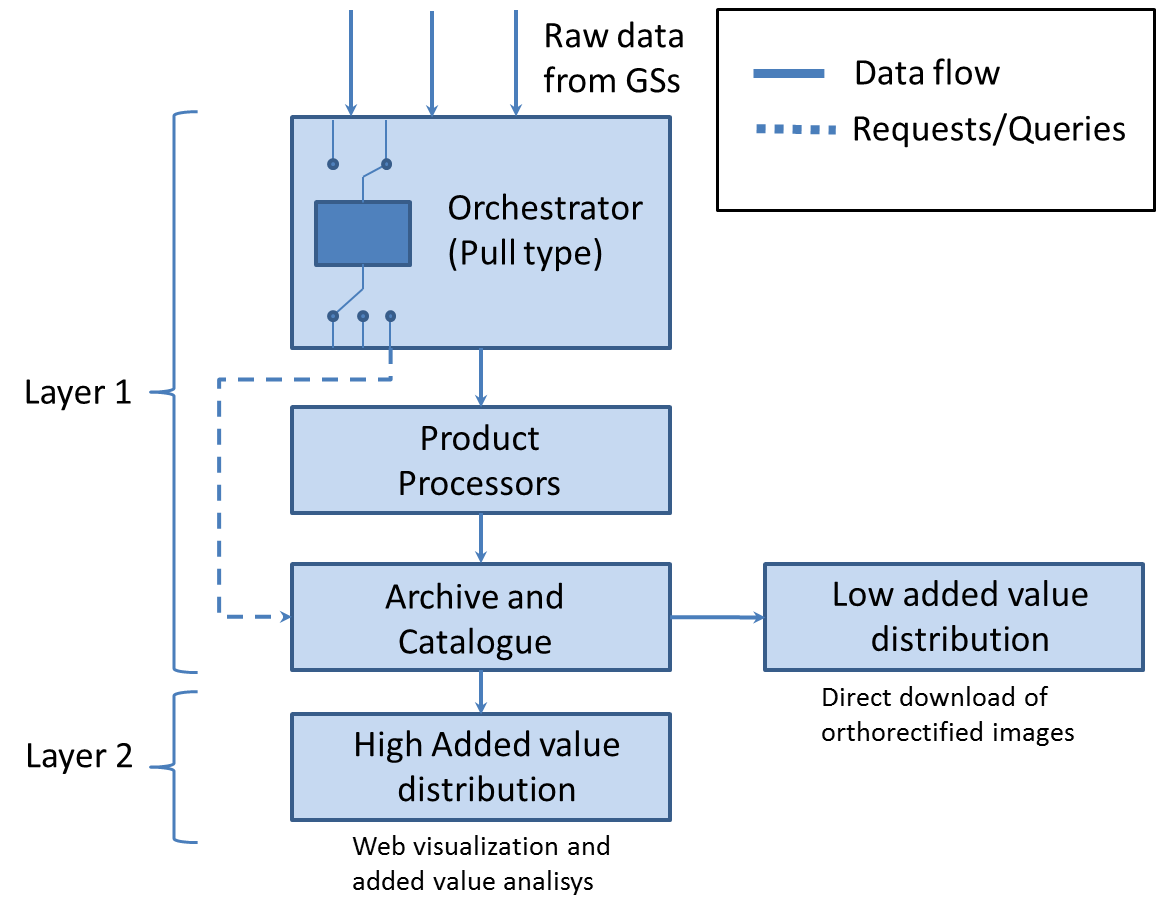
\includegraphics[width=5.01448in,height=3.96902in]{out-img33.png} \par}

{\centering\bfseries
\label{bkm:Ref378074782}Figure\ 25. Data Processing in Cloud.
\par}


\bigskip

The data flow is depicted in a numbered sequence as follows:

\liststyleLFOxxxiii
\setcounter{saveenum}{\value{enumi}}
\begin{enumerate}
\setcounter{enumi}{\value{saveenum}}
\item Data Ingestion. Incoming data is ingested into the system. The
main source for incoming data is from the satellites. However, there
can be other input sources, such as the calibration\ facility.
Depending on the nature of the incoming data, some pre-processing might
be required. In all cases, the incoming data is incorporated to the
Archive. This operation is directed by the Orchestrator.
\item The Orchestrator, driven by the event of new data ingested,
follows a set of rules, or task tables, to initiate the execution of a
Processor whenever all the inputs are available. When the input files
are all available the Orchestrator circulates them to a (shared
{\textless}{\textless}TBD{\textgreater}{\textgreater}) storage area.
\item Once all the files are ready for processing in the storage area,
the Orchestrator prepares a Job Order for the Product Processors. The
Job Order contains all the information required by the Processing
Facility to process incoming data. The Orchestrator starts and controls
the execution of the Processor required to perform the Job Order.\ 
\item The Processor retrieves data from the storage area and performs
the required process on the input data, generating output data in the
shared storage area. The execution of a Processor is specified in the
Job Order. During the execution, the Processor logs the most
significant events occurring during the processing.
\item Upon finalization, the Orchestrator moves the produced data into
the Archive.
\item From the archive, data can be delivered and transformed into more
specific products and value added services though FTP, Web Services,
OGC Standard Web Services, etc.\ 
\end{enumerate}

\bigskip

\subsection[Orchestrator]{Orchestrator}
\hypertarget{Toc381777211}{}
\bigskip

The orchestrator has the following functions:


\bigskip

\liststyleLFOxxvi
\begin{itemize}
\item Understanding of the processors capabilities:

\begin{itemize}
\item Identifies if the input is mandatory or optional
\item It identifies which outputs shall be generated by the processors
\end{itemize}
\item Generating the Job Orders: they contain all the necessary
information that the processors need. They include the interfaces and
addresses of the folders in which the input information for the
processors is located and the folders in which the outputs of the
processors have to be sent. They also include the format in which the
processors generate their output. They are XML files.
\item Reading the configuration of the processor chain to obtain the
information about the type of orders that can be attended with their
priority and the processors to be launched during all the processing
chain.
\item Controlling the processors to instruct them to pause, resume and
cancel the operation.
\end{itemize}

\bigskip

The orchestrator receives the information in a pull type manner. It is
the input interface to the cloud from the ground stations. The
orchestrator is looking at the\ FTPs that connect the ground stations
with the cloud and if there is data it takes it and manages it to the
processing chain through Job Orders.


\bigskip

The Orchestrator has to be implemented in a Virtual Machine. From this
VM the processing chain is managed.\ 


\bigskip

The following table shows the instance type that is intended to use for
the orchestrator.


\bigskip

\begin{center}
\tablehead{}
\begin{supertabular}{|m{1.0010599in}|m{1.5198599in}|m{1.5205599in}|m{1.5205599in}|}
\hline
\centering \bfseries Instance type &
\centering \bfseries CPU cores &
\centering \bfseries Memory &
\centering\arraybslash \bfseries Features\\\hline
\centering medium &
\centering 2 &
\centering 2GB &
~
\\\hline
\end{supertabular}
\end{center}

\bigskip

The orchestrator will be ad hoc implemented for BonFIRE as our first
option.\ 

\subsection[Product Processors]{Product Processors}
\hypertarget{Toc381777212}{}
\bigskip

The Product Processors is\ a module\ that is in charge of processing the
payload raw data from the satellites\ to produce image products. The
four, most important operations that the product processors perform on
the input data are\ the following:

\liststyleLFOxxvii
\begin{itemize}
\item A calibration, to convert the pixel elements from instrument
digital counts into radiance units.
\item A geometric correction, to eliminate distortions due to
misalignments of the sensors in the focal plane geometry.
\item A geolocation, to compute the geodetic coordinates of the input
pixels.
\item An ortho-rectification, to produce ortho-photos with vertical
projection, free of distortions.
\end{itemize}

\bigskip

The previous steps also generate quality-related figures of merit that
are made available in all the products. Moreover, the product
processors generate metadata, in line with industry standards, to
facilitate the cataloguing, filtering and browsing of the product image
collection.


\bigskip

The output image products are classified into\ four\ different levels,
according to the degree of processing that they have been subjected
to\ (see\ Figure 26):


\bigskip

\liststyleLFOxxviii
\begin{itemize}
\item Level 0 products are unprocessed images, in digital count numbers.
\item Level 1A products are calibrated products, in units of radiance.
\item Level 1B products are calibrated and geometrically corrected
products (ortho-rectified), blindly geolocated.
\item Level 1C products are calibrated and geometrically corrected
products (ortho-rectified), precisely geolocated using ground control
points.
\end{itemize}
{\centering 
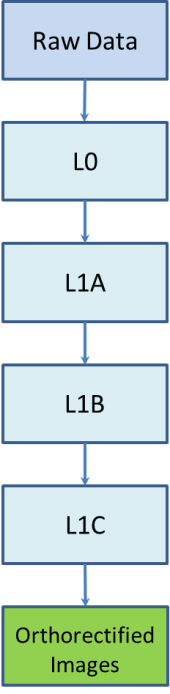
\includegraphics[width=0.77326in,height=3.15694in]{out-img34.png} \par}

{\centering\bfseries
\label{bkm:Ref378175274}Figure\ 26.\ Stages of product processing.
\par}


\bigskip


\bigskip

All the processing chain, i.e., the four processors will be installed in
one Virtual Machine. The orchestrator will manage the running of
different VMs with the processors replicated for parallel processing of
different images at the same time.


\bigskip

The instance type in which the processors will be implemented should
have at least the following characteristics:


\bigskip

\begin{center}
\tablehead{}
\begin{supertabular}{|m{1.0010599in}|m{1.5198599in}|m{1.5205599in}|m{1.5205599in}|}
\hline
\centering \bfseries Instance type &
\centering \bfseries CPU cores &
\centering \bfseries Memory &
\centering\arraybslash \bfseries Features\\\hline
\centering xlarge+ &
\centering 4 &
\centering 8GB &
\centering\arraybslash \textrm{Higher CPU clock speed (over
3GHz)}\\\hline
\end{supertabular}
\end{center}

\bigskip


\bigskip

In the scenarios that will be tested in the experiment the worst case is
that in which twelve satellites will be downloading data to ground
stations simultaneously. Thus twelve nodes with replicated processors
will process images simultaneously.


\bigskip


\bigskip

{\centering 
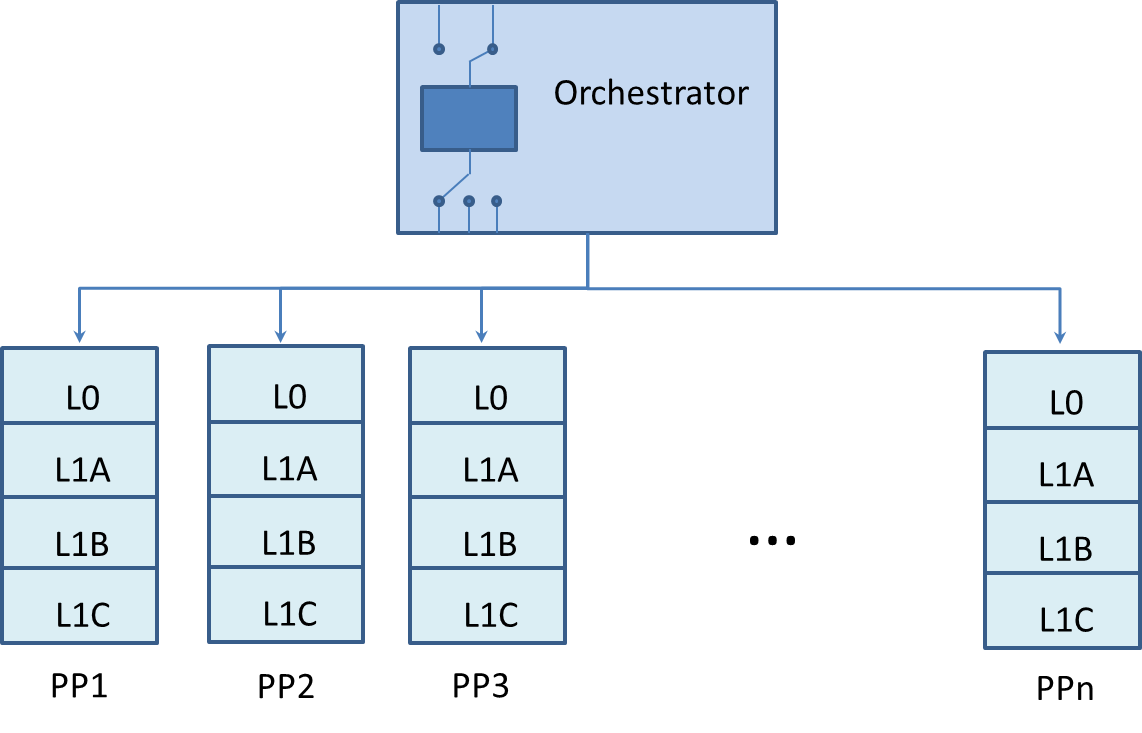
\includegraphics[width=5.05745in,height=3.24601in]{out-img35.png} \par}

{\centering\bfseries
Figure\ 27.\ Scheme of the orchestrator managing different product
processors in parallel.
\par}


\bigskip

The product processors are four .exe files, one per processing stage.
They will be configured via XML files. Not compilation of the software
will be required, just interpretation of the configuration files.


\bigskip

The Product Processors software requirements are the following in our
premises:

\liststyleLFOxxix
\begin{itemize}
\item Linux Operative System
\item Virtual environment VMware
\item CentOS
\end{itemize}
For their implementation in BonFIRE we will study the following
possibility:

\liststyleLFOxxx
\begin{itemize}
\item The implementation of the product processors in the BonFIRE cloud
through its interface to automatically and dynamically provision new
VMs. This means that the first approach will be not to access the
BonFIRE hypervisor as a backend, nor deploying the VMware hypervisor
for example in\ be-ibbt is running physical nodes, and could provide
this possibility\ (Xeon E5645 supports VT-d technology). This
implementation will make the system flexible and scalable. Thus the
executor will be able of provisioning new instances for an on-demand
use of the resources. In conclusion, we will compute the Virtual
Machines and we will not deploy\ VMware.\ 
\item In BonFIRE, centOS is a feature not already implemented, although
contemplated. Not to depend on this we will run the software on Debian
Squeeze.
\end{itemize}

\bigskip

\subsubsection[The L0 processor]{The L0 processor}
\hypertarget{Toc381777213}{}
\bigskip

The acquired data is organized into image sectors of predefined size and
structure\ and converted in scenes. Scenes, as defined here, are used
throughout the subsequent L1 levels. The size and configuration of the
scene is not changed again in the processing chain, for this reason the
scene definition is constant for all the L1 levels.


\bigskip

The inputs are the following

\liststyleLFOxxxii
\begin{itemize}
\item The Raw Data.
\item The configuration database.
\item The calibration database.
\end{itemize}

\bigskip

The outputs are the following:

\liststyleLFOxxxii
\begin{itemize}
\item The L0 products.
\end{itemize}

\bigskip


\bigskip

\subsubsection[The L1A processor]{The L1A processor}
\hypertarget{Toc381777214}{}
\bigskip

This section describes the functionality of the processors included in
the Level 1A of the Automatic Processing Chain. The goal of Level 1A is
to calibrate the scenes. The resulting images are given in units of
radiances.\ 


\bigskip

The L1A component works on the scenes that compound the L0 product,
performing different transformations over pixel values to generate
radiances.


\bigskip

The inputs to the L1A level are:

\liststyleLFOxxxii
\begin{itemize}
\item One L0 scene.
\item The configuration database.
\item The calibration database.
\end{itemize}

\bigskip

The output is:

\liststyleLFOxxxii
\begin{itemize}
\item The L1A product.
\end{itemize}

\bigskip

\subsubsection[The L1B processor]{The L1B processor}
\hypertarget{Toc381777215}{}
\bigskip

Level 1B implements the geolocation, resampling and packing.


\bigskip

The inputs to the L1B level are the following:

\liststyleLFOxxxii
\begin{itemize}
\item The L1A product.
\item The configuration database.
\item The calibration database.
\end{itemize}

\bigskip

The outputs are the following:

\liststyleLFOxxxii
\begin{itemize}
\item The L1B products.
\end{itemize}

\bigskip

\subsubsection[The L1C processor]{The L1C processor}
\hypertarget{Toc381777216}{}
\bigskip

The L1C processor performs the ortho-rectification of the L1B product
using ground control points.


\bigskip

The inputs to the L1C level are the following:

\liststyleLFOxxxii
\begin{itemize}
\item The L1B\ product.
\item The calibration database.
\item The configuration database.
\end{itemize}

\bigskip

The output is the following:

\liststyleLFOxxxii
\begin{itemize}
\item The L1C products.
\end{itemize}

\bigskip


\bigskip

\subsection[Archive and Catalogue]{Archive and Catalogue}
\hypertarget{Toc381777217}{}
\bigskip

The archive and catalog is a shared space of memory between the
orchestrator, the product processors and the distribution of data. It
has a data acquisition component.


\bigskip

\textbf{Data Acquisition component}: This component manages the input
data arriving to the Archive and Catalog. The ingestion of data is
automatic.\ 


\bigskip

In the Archive and Catalog module the processed images will be stored
and catalogued for their distribution in both ways direct downloading
(low added value services) and web based service (high added value
services).


\bigskip

{\color{black}
The Archive and Catalog basically consists of:}


\bigskip

\liststyleLFOxxxi
\begin{itemize}
\item {\color{black}
The Archive is constituted by optimized storages structure allowing
managing a big amount of data, efficient storage and retrieval of any
kind of file. The Archive shall be organized in hierarchical levels of
storage in order to provide a cost effective storage solution.}
\end{itemize}

\bigskip

\liststyleLFOxxxi
\begin{itemize}
\item {\color{black}
The Catalogue shall store an inventory database with the metadata of
archive files. It allows the product process chain easiness to access
to the metadata from the processed products.}
\end{itemize}

\bigskip

\liststyleLFOxxxi
\begin{itemize}
\item {\color{black}
For the added value services the catalog will be accessed by a Web
Service.}
\end{itemize}

\bigskip

\liststyleLFOxxxi
\begin{itemize}
\item \textcolor{black}{CSW (Catalog Service for the Web) is a module
with the CSW standard for the catalogue (based on OGC
standard).}\textcolor[rgb]{0.14901961,0.14509805,0.13725491}{\ For more
information on CSW, please refer
to}\textcolor[rgb]{0.14901961,0.14509805,0.13725491}{~}\href{http://www.opengeospatial.org/standards/specifications/catalog}{\textcolor[rgb]{0.0,0.4627451,0.6313726}{OGC
OpenGIS Implementation Specification
07-006r1}}\textcolor[rgb]{0.14901961,0.14509805,0.13725491}{~}\textcolor[rgb]{0.14901961,0.14509805,0.13725491}{and
the\ }\href{http://www.ogcnetwork.net/node/630}{\textcolor[rgb]{0.0,0.4627451,0.6313726}{OGC
tutorial on
CSW}}\textcolor[rgb]{0.14901961,0.14509805,0.13725491}{.}\textcolor{black}{\ Through
this standard\ }\textcolor{black}{the distribution of data is done. It
communicates with the Archive and Catalog. We intend to use GeoServer
and GeoNetwork:}
\end{itemize}
\textcolor{black}{GeoServer:\ }\url{http://docs.geoserver.org/latest/en/user/extensions/csw/index.html}

\textcolor{black}{GeoNetwork:\ }\url{http://geonetwork-opensource.org/}


\bigskip


\bigskip

{\centering 
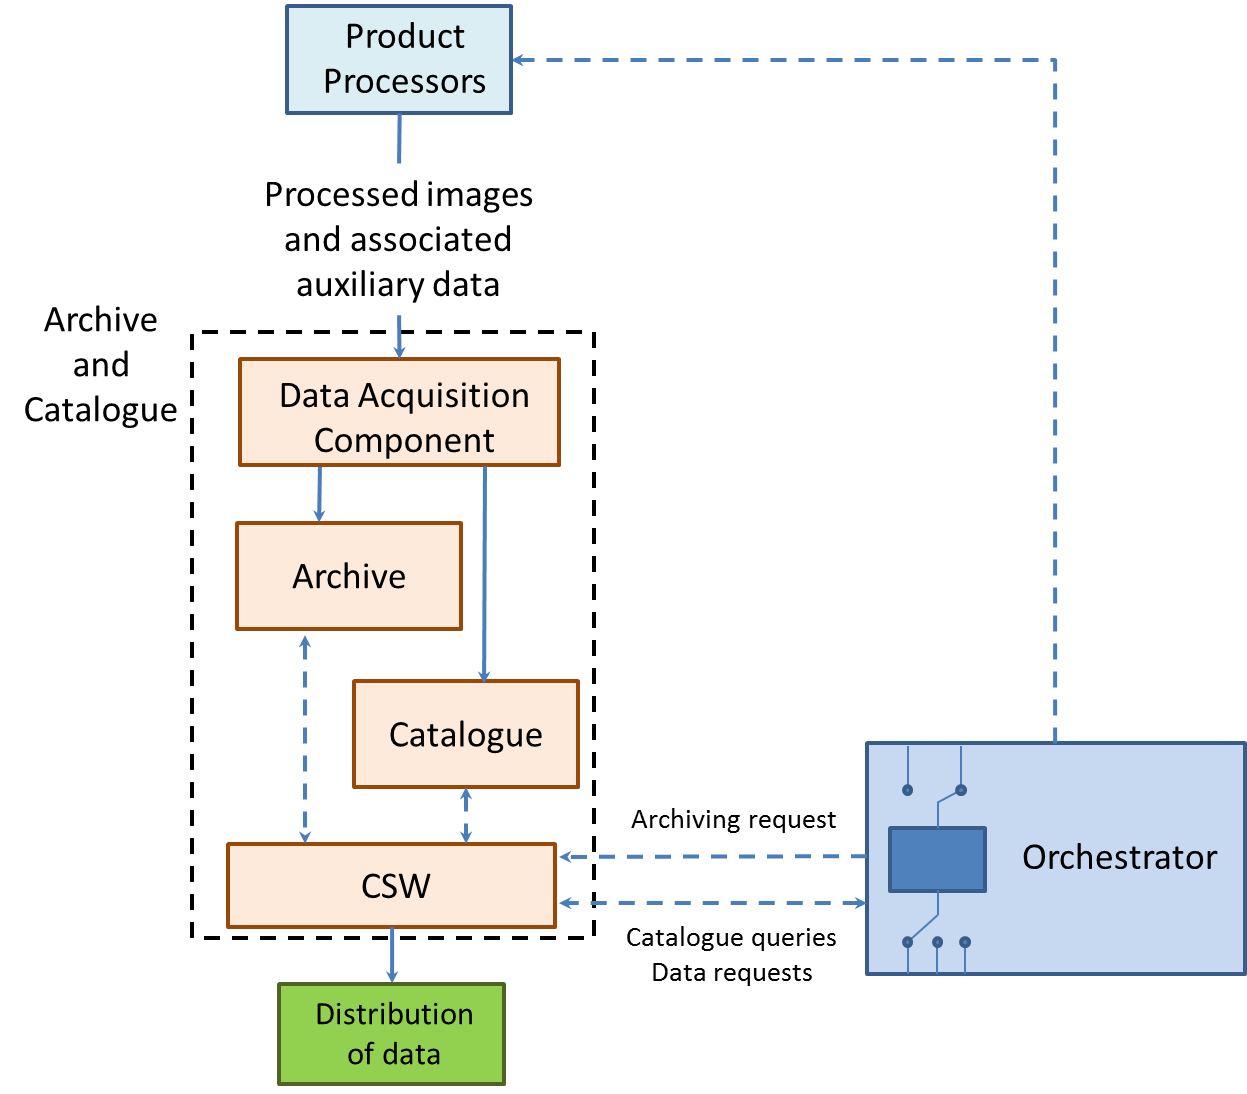
\includegraphics[width=4.49882in,height=3.9468in]{out-img36.png} \par}

{\centering\bfseries
Figure\ 28.\ Scheme of the Archive and Catalogue Module.
\par}


\bigskip

Instance required for archive and catalogue:\ 


\bigskip

\begin{center}
\tablehead{}
\begin{supertabular}{|m{1.0010599in}|m{1.5198599in}|m{1.5205599in}|m{1.5205599in}|}
\hline
\centering \bfseries Instance type &
\centering \bfseries CPU cores &
\centering \bfseries Memory &
\centering\arraybslash \bfseries Features\\\hline
\centering storage &
\centering {}- &
\centering TBD &
~
\\\hline
\end{supertabular}
\end{center}

\bigskip

\subsection[Imagery Distribution and Visualization]{Imagery Distribution
and Visualization}
\hypertarget{Toc381777218}{}The architecture of the Imagery distribution
and visualization was depicted in\ Section\ 4. The Archive and Catalog
provides the processed satellite images to a raster and a vector
datastore that ingest the data into an\ EO server for its later
distribution to the end user.\ \ In the following subsections the
modules of the architecture will be briefly described. The resources
that will be required in BonFIRE are also depicted\ in tables.\ More
information about imagery distribution and visualization can be found
in Section\ 4.

\subsubsection[Archive and Catalogue]{Archive and Catalogue}
\hypertarget{Toc381777219}{}The processed images will be stored and
catalogued for their distribution in both ways direct downloading (low
added value services) and web based service (high added value
services).

\subsubsection[Datastore]{Datastore}
\hypertarget{Toc381777220}{}The datastore will be fed from the archive
and catalogue with the required scenes from the archive. In some cases,
additional processing will be needed to optimize these scenes for
distribution through OGC Web Services, to populate the tiles cache,
etc.


\bigskip

\begin{center}
\tablehead{}
\begin{supertabular}{|m{1.0010599in}|m{1.5198599in}|m{1.5205599in}|m{1.5205599in}|}
\hline
\centering \bfseries Instance type &
\centering \bfseries CPU cores &
\centering \bfseries Memory &
\centering\arraybslash \bfseries Features\\\hline
\centering storage &
\centering {}- &
\centering \ 300 GB &
~
\\\hline
\end{supertabular}
\end{center}

\bigskip

The datastore will be based on two components:

\liststyleLFOxxiii
\begin{itemize}
\item A geospatial database, to handle geometries and vector features,
and in some cases, raster files. It will be based on PostGIS database.
\item The instance filesystem.
\end{itemize}
\subsubsection[EO Server]{EO Server}
\hypertarget{Toc381777221}{}A map and feature server for sharing,
analyzing, and editing geospatial data from spatial data sources using
open standards. It implements OGC Web Services (WMS, WFS, WCS, etc.) as
well as providing tiling and cache mechanisms.\ 

For most of its web services, it can be scaled horizontally by adding
several EO Server nodes to the infrastructure.\ 


\bigskip

\begin{center}
\tablehead{}
\begin{supertabular}{|m{1.0010599in}|m{1.5198599in}|m{1.5205599in}|m{1.5205599in}|}
\hline
\centering \bfseries Instance type &
\centering \bfseries CPU cores &
\centering \bfseries Memory &
\centering\arraybslash \bfseries Features\\\hline
\centering \textrm{\textcolor{black}{xlarge+}} &
\centering 4 &
\centering \ 8GB &
Higher CPU clock speed (over 3GHz)\\\hline
\end{supertabular}
\end{center}

\bigskip

\begin{center}
\tablehead{}
\begin{supertabular}{|m{1.0010599in}|m{1.5198599in}|m{1.5205599in}|m{1.5205599in}|}
\hline
\centering \bfseries Instance type &
\centering \bfseries CPU cores &
\centering \bfseries Memory &
\centering\arraybslash \bfseries Features\\\hline
\centering Load balancer &
\centering {}- &
\centering \ {}- &
\centering\arraybslash EaaS\\\hline
\end{supertabular}
\end{center}

\bigskip

\subsubsection[Tiles Caches]{Tiles Caches}
\hypertarget{Toc381777222}{}For the tiles cache,\ GeoWebCache\ will be
used.\ \ It is\ s a Java web application used to cache map tiles coming
from a variety of sources such as OGC Web Map Service (WMS). It
implements various service interfaces (such as WMS-C, WMTS, TMS, Google
Maps KML, Virtual Earth) in order to accelerate and optimize map image
delivery. It can also recombine tiles to work with regular WMS clients.

GeoWebCache can scale horizontally by adding nodes sharing the same
cache data store. To store the cached tiles, high storage capacity is
needed.


\bigskip

\begin{center}
\tablehead{}
\begin{supertabular}{|m{1.0010599in}|m{1.5198599in}|m{1.5205599in}|m{1.5205599in}|}
\hline
\centering \bfseries Instance type &
\centering \bfseries CPU cores &
\centering \bfseries Memory &
\centering\arraybslash \bfseries Features\\\hline
\centering storage &
\centering {}- &
\centering \ 500 GB &
~
\\\hline
\end{supertabular}
\end{center}

\bigskip

\begin{center}
\tablehead{}
\begin{supertabular}{|m{1.0010599in}|m{1.5198599in}|m{1.5205599in}|m{1.5205599in}|}
\hline
\centering \bfseries Instance type &
\centering \bfseries CPU cores &
\centering \bfseries Memory &
\centering\arraybslash \bfseries Features\\\hline
\centering Custom &
\centering 4 &
\centering \ 2GB &
Higher CPU clock speed (over 3GHz)\\\hline
\end{supertabular}
\end{center}

\bigskip

\begin{center}
\tablehead{}
\begin{supertabular}{|m{1.0010599in}|m{1.5198599in}|m{1.5205599in}|m{1.5205599in}|}
\hline
\centering \bfseries Instance type &
\centering \bfseries CPU cores &
\centering \bfseries Memory &
\centering\arraybslash \bfseries Features\\\hline
\centering Load balancer &
\centering {}- &
\centering \ {}- &
\centering\arraybslash EaaS\\\hline
\end{supertabular}
\end{center}

\bigskip

\subsection[Data, control and monitoring parameters]{Data, control and
monitoring parameters}
\hypertarget{Toc381777223}{}
\bigskip

\subsubsection[Data]{Data}
\hypertarget{Toc381777224}{}The data that will be transferred between
nodes. It will be images of about 2GB size.


\bigskip

\subsubsection[Control parameters]{Control parameters}
\hypertarget{Toc381777225}{}
\bigskip

The control parameters are the inputs from Virtual Wall:


\bigskip

\begin{center}
\tablehead{}
\begin{supertabular}{|m{2.4677598in}|}
\hline
\centering\arraybslash \bfseries BonFIRE control parameters\\\hline
\centering\arraybslash GS\# servers\\\hline
\centering\arraybslash User\# clients\\\hline
\end{supertabular}
\end{center}

\bigskip

\subsubsection[Monitoring parameters]{Monitoring parameters}
\hypertarget{Toc381777226}{}
\bigskip

The monitoring parameters are depicted in the following table:


\bigskip


\bigskip

\begin{center}
\tablehead{}
\begin{supertabular}{|m{2.4677598in}|}
\hline
\centering\arraybslash \bfseries BonFIRE monitoring parameters\\\hline
\centering\arraybslash Processing time\\\hline
\centering\arraybslash Latency from image capture to
distribution\\\hline
\centering\arraybslash Storage load\\\hline
\centering\arraybslash Processing load\\\hline
\centering\arraybslash Processing and storage strategy viability\\\hline
\centering\arraybslash Cues management\\\hline
\centering\arraybslash Performance of the system\\\hline
\end{supertabular}
\end{center}

\bigskip


\bigskip

\subsection[Data flow and configuration of the nodes]{Data flow and
configuration of the nodes}
\hypertarget{Toc381777227}{}
\bigskip

The data flow is the following:

\liststyleLFOxxxv
\setcounter{saveenum}{\value{enumi}}
\begin{enumerate}
\setcounter{enumi}{\value{saveenum}}
\item The BonFIRE cloud acts as a client to the GS servers in Virtual
Wall. Both are interconnected through an\ FTP.
\item The orchestrator pulls over the
{\textquotedblleft}GS\#{\textquotedblright} servers in Virtual Wall if
there is data available it is ingested into the processing chain
computed in the BonFIRE cloud.
\item Once the data has been processed and images have been stored they
are distributed from the BonFIRE cloud servers to the Virtual Wall
clients named as {\textquotedblleft}User\#{\textquotedblright}.
\ \ There are two options:

\setcounter{saveenum}{\value{enumii}}
\begin{enumerate}
\setcounter{enumii}{\value{saveenum}}
\item A User\# client pulls over the BonFIRE servers via\ FTP or
SSH\ and retrieve the data.
\item A BonFIRE server pushes (transfers) the data over a User\# client.
It is usually done using Web Services (OGC, REST, HTTP).\ 
\end{enumerate}
\item A hosting service from BonFIRE is also provided to the User\#
Clients in Virtual Wall.
\end{enumerate}
See\ Figure 29\ for a graphical description of the data flow and
configuration of the nodes.


\bigskip

{\centering 
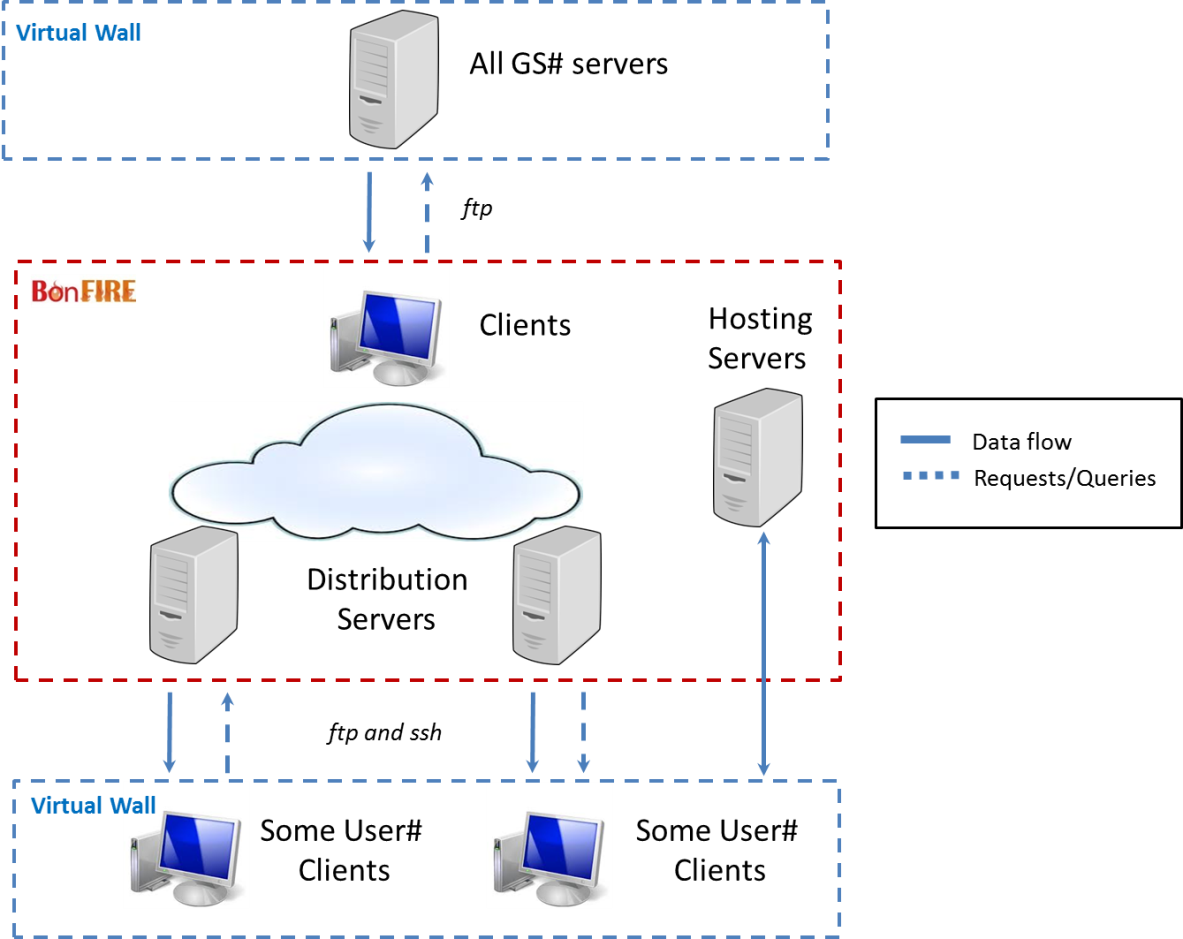
\includegraphics[width=5.38496in,height=4.27496in]{out-img37.png} \par}

{\centering\bfseries
\label{bkm:Ref378755152}Figure\ 29.\ Data flow and configuration of the
nodes.
\par}


\bigskip

\subsection[Summary]{Summary}
\hypertarget{Toc381777228}{}
\bigskip

In this document the architecture to be implanted in the BonFIRE cloud
has been described. The resources to be used during the implementation
and the experimentation were defined. The connectivity between Virtual
Wall and BonFIRE were introduced.


\bigskip

The software modules to be installed in BonFIRE and the scripts and
software to be developed in order to integrate the experiment were
defined.

\section[Topology Networks in Virtual Wall]{Topology Networks in Virtual
Wall}
\label{bkm:Ref378931913}\hypertarget{Toc381777229}{}
\bigskip

In this section the topology networks to be implemented in Virtual Wall
for the execution of the GEO-Cloud experiment are designed.\ 


\bigskip

Virtual Wall will communicate with the BonFIRE cloud in two manners:

\liststyleLFOxxxviii
\setcounter{saveenum}{\value{enumi}}
\begin{enumerate}
\setcounter{enumi}{\value{saveenum}}
\item Transferring data from Virtual Machines in Virtual Wall to the
BonFIRE cloud.
\item Requesting data to the BonFIRE cloud and receiving it to the
Virtual Wall servers.
\end{enumerate}
The option {\textquotedblleft}a{\textquotedblright} emulates the
transfer of data from satellites to ground stations located around the
world and such data transferred to the BonFIRE cloud.


\bigskip

The option {\textquotedblleft}b{\textquotedblright} emulates the
requesting of low and high added value GEO-Cloud services from users
around the world.


\bigskip

Figure 30\ shows the relation between Virtual Wall and BonFIRE.


\bigskip


\bigskip

{\centering 
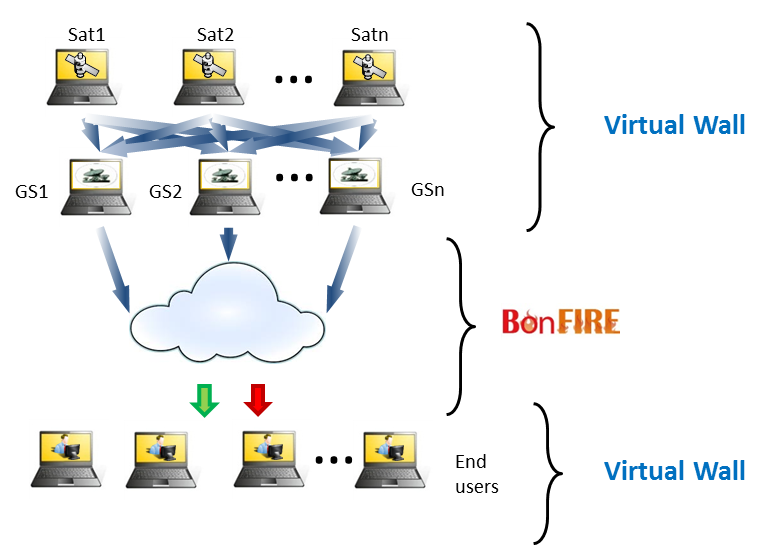
\includegraphics[width=4.20349in,height=2.99424in]{out-img38.png} \par}

{\centering\bfseries
\label{bkm:Ref378262923}Figure\ 30.\ Communication between VW and BF.
\par}

\subsection[Architecture]{Architecture}
\hypertarget{Toc381777230}{}
\bigskip

The system to be implemented in Virtual Wall is constituted by three
layers:

\liststyleLFOxxxvi
\begin{itemize}
\item In layer 1: 17 nodes will be used to simulate 17 satellites in
orbit.
\item In layer 2: 12 nodes will be used to simulate 12 ground stations
in which data is transferred from layer 1. The data transferred to
layer 2 is transferred to the BonFIRE cloud.
\item In layer 3: n (TBD) nodes will be used to emulate n (TBD) users
requesting data from the BonFIRE Cloud.
\end{itemize}

\bigskip


\bigskip

{\centering 
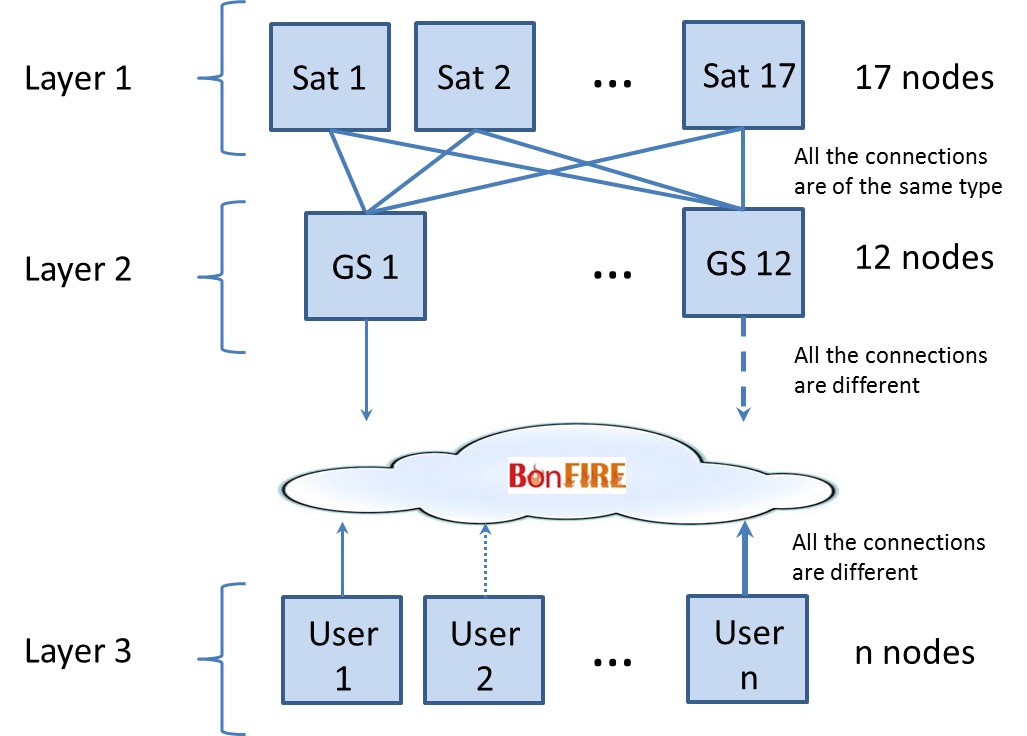
\includegraphics[width=5.06254in,height=3.62798in]{out-img39.png} \par}

{\centering\bfseries
Figure\ 31.\ Architecture implemented in Virtual Wall.
\par}


\bigskip


\bigskip

\subsection[Layer 1]{Layer 1}
\hypertarget{Toc381777231}{}
\bigskip

To constitute the layer 1 we need 17 nodes. In every node a script will
be computed to emulate the recordings of a satellite, its orbit and its
passes over ground stations.


\bigskip

The data to be transferred from layer 1 to layer 2 will be lower than
60GB. The data to be transferred will be raw data satellite imagery of
about 2GB each.


\bigskip

Every Sat node is connected with all the GS nodes. All the links between
a Sat node and a GS node have the same features: 160 Mbps bandwidth
with impairments (measured in reality with the Deimos{\textquoteright}
satellites). In total there are 204 links between the Sat and the GS
nodes. Every Sat node is acting as a server and every GS node as a
client.


\bigskip

{\centering 
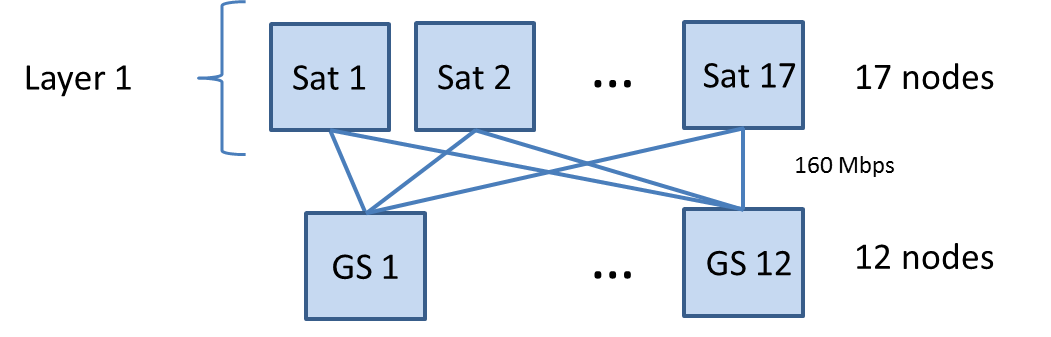
\includegraphics[width=4.94458in,height=1.5853in]{out-img40.png} \par}

{\centering\bfseries
Figure\ 32.\ Layer 1 resources.
\par}


\bigskip

We have 17 subnets of the following type:


\bigskip


\bigskip

{\centering 
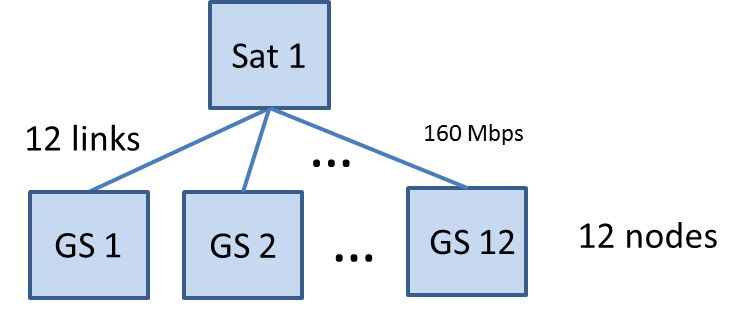
\includegraphics[width=3.6049in,height=1.5545in]{out-img41.png} \par}

{\centering\bfseries
Figure\ 33.\ Subnet between the node Sat1 and the nodes GS1 to GS12.
\par}


\bigskip

Resources required for Layer 1:\ 


\bigskip

\begin{center}
\tablehead{}
\begin{supertabular}{|m{0.8767598in}|m{1.0823599in}|m{1.1656599in}|m{0.95035976in}|m{0.95035976in}|m{0.95035976in}|}
\hline
\centering \bfseries Nodes \& Resources &
\centering \bfseries Number &
\centering \bfseries Bandwidth &
\centering \bfseries Latency &
\centering \bfseries Loss Rate &
\centering\arraybslash \bfseries Background Traffic\\\hline
\centering Nodes &
\centering 17 &
\centering {}- &
\centering {}- &
\centering {}- &
\centering\arraybslash {}-\\\hline
\centering Resources &
\centering 12 &
\centering 160Mbps &
\centering 2.15ms &
\centering 10e-6 &
\centering\arraybslash 0\\\hline
\end{supertabular}
\end{center}

\bigskip


\bigskip

Description of the subnets in layer 1:


\bigskip

Subnet 1: 172.16.1.0

Subnet 2: 172.16.2.0

Subnet 3: 172.16.3.0

Subnet 4: 172.16.4.0

Subnet 5: 172.16.5.0

Subnet 6: 172.16.6.0

Subnet 7: 172.16.7.0

Subnet 8: 172.16.8.0

Subnet 9: 172.16.9.0

Subnet 10: 172.16.10.0

Subnet 11: 172.16.11.0

Subnet 12: 172.16.12.0

Subnet 13: 172.16.13.0

Subnet 14: 172.16.14.0

Subnet 15: 172.16.15.0

Subnet 16: 172.16.16.0

Subnet 17: 172.16.17.0


\bigskip

\subsection[Layer 2]{Layer 2}
\hypertarget{Toc381777232}{}
\bigskip

Layer 2 is constituted by 12 nodes named GS\# nodes. Every node is
representing a ground station. The ground stations connect with the
satellites and receive data. But they also act as servers to transfer
the previous data to the BonFIRE cloud. The connectivity between GS\#
and BonFIRE will be\ FTP.


\bigskip

{\centering 
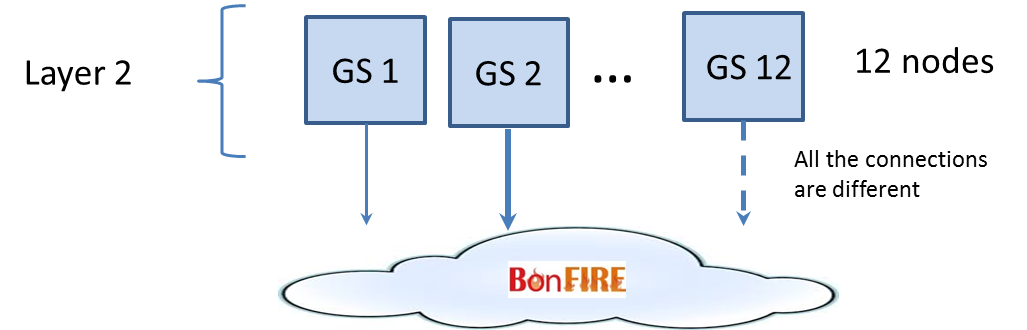
\includegraphics[width=5.41165in,height=1.73875in]{out-img42.png} \par}

{\centering\bfseries
Figure\ 34.\ Layer 2.
\par}


\bigskip

We have other 12 subnets, but in this case every GS node has one
connection with the cloud.


\bigskip

Resources required for Layer 2:\ 


\bigskip

\begin{center}
\tablehead{}
\begin{supertabular}{|m{0.8767598in}|m{1.0823599in}|m{1.1656599in}|m{0.95035976in}|m{0.95035976in}|m{0.95035976in}|}
\hline
\centering \bfseries Nodes \& Resources &
\centering \bfseries Number &
\centering \bfseries Bandwidth &
\centering \bfseries Latency &
\centering \bfseries Loss Rate &
\centering\arraybslash \bfseries Background Traffic\\\hline
\centering Nodes &
\centering 12 &
\centering {}- &
\centering {}- &
\centering {}- &
\centering\arraybslash {}-\\\hline
\centering Resources &
\centering 1 &
\centering TBD\  &
\centering TBD &
\centering TBD &
\centering\arraybslash TBD\\\hline
\centering Resources &
\centering 1 &
\centering TBD\  &
\centering TBD &
\centering TBD &
\centering\arraybslash TBD\\\hline
\centering Resources &
\centering 1 &
\centering TBD\  &
\centering TBD &
\centering TBD &
\centering\arraybslash TBD\\\hline
\centering Resources &
\centering 1 &
\centering TBD\  &
\centering TBD &
\centering TBD &
\centering\arraybslash TBD\\\hline
\centering Resources &
\centering 1 &
\centering TBD\  &
\centering TBD &
\centering TBD &
\centering\arraybslash TBD\\\hline
\centering Resources &
\centering 1 &
\centering TBD\  &
\centering TBD &
\centering TBD &
\centering\arraybslash TBD\\\hline
\centering Resources &
\centering 1 &
\centering TBD\  &
\centering TBD &
\centering TBD &
\centering\arraybslash TBD\\\hline
\centering Resources &
\centering 1 &
\centering TBD\  &
\centering TBD &
\centering TBD &
\centering\arraybslash TBD\\\hline
\centering Resources &
\centering 1 &
\centering TBD\  &
\centering TBD &
\centering TBD &
\centering\arraybslash TBD\\\hline
\centering Resources &
\centering 1 &
\centering TBD\  &
\centering TBD &
\centering TBD &
\centering\arraybslash TBD\\\hline
\centering Resources &
\centering 1 &
\centering TBD\  &
\centering TBD &
\centering TBD &
\centering\arraybslash TBD\\\hline
\centering Resources &
\centering 1 &
\centering TBD\  &
\centering TBD &
\centering TBD &
\centering\arraybslash TBD\\\hline
\end{supertabular}
\end{center}

\bigskip


\bigskip

The bandwidth and impairments for each subnet is still TBD, although all
of them will be different. In the experiment we will fit initial values
for each of them that will later be updated with the measurements we
will obtain from real measurements in PlanetLab Europe.


\bigskip

Description of the subnets in layer 2:


\bigskip

Subnet 18: 172.16.18.0

Subnet 19: 172.16.19.0

Subnet 20: 172.16.20.0

Subnet 21: 172.16.21.0

Subnet 22: 172.16.22.0

Subnet 23: 172.16.23.0

Subnet 24: 172.16.24.0

Subnet 25: 172.16.25.0

Subnet 26: 172.16.26.0

Subnet 27: 172.16.27.0

Subnet 28: 172.16.28.0

Subnet 29: 172.16.29.0


\bigskip


\bigskip

\subsection[Layer 3]{Layer 3}
\hypertarget{Toc381777233}{}
\bigskip

Layer 3 is constituted by n (TBD) nodes ({\textless}10 probably) with
computed scripts that will be emulating end users loads (requests and
data transfer from the BonFIRE cloud). The data transfer can be of two
types:

\liststyleLFOxxxvii
\setcounter{saveenum}{\value{enumi}}
\begin{enumerate}
\setcounter{enumi}{\value{saveenum}}
\item Direct download of data through (FTP)
\item Visualization through a web service (HTTP).
\end{enumerate}

\bigskip

Every node will have a defined type of data transfer. They are still
TBD.\ 


\bigskip

{\centering 
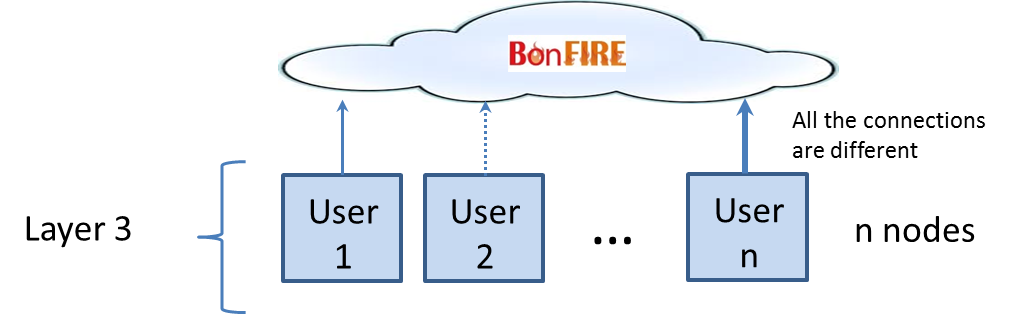
\includegraphics[width=5.04475in,height=1.54557in]{out-img43.png} \par}

{\centering\bfseries
Figure\ 35.\ Layer 3.
\par}


\bigskip

Resources required for Layer 3:\ 


\bigskip

\begin{center}
\tablehead{}
\begin{supertabular}{|m{0.8767598in}|m{1.0823599in}|m{1.1656599in}|m{0.95035976in}|m{0.95035976in}|m{0.95035976in}|}
\hline
\centering \bfseries Nodes \& Resources &
\centering \bfseries Number &
\centering \bfseries Bandwidth &
\centering \bfseries Latency &
\centering \bfseries Loss Rate &
\centering\arraybslash \bfseries Background Traffic\\\hline
\centering Nodes &
\centering N (TBD {\textless}10) &
\centering {}- &
\centering {}- &
\centering {}- &
\centering\arraybslash {}-\\\hline
\centering Resources &
\centering 1 &
\centering TBD\  &
\centering TBD (from experiments in \ PlanetLab Europe) &
\centering TBD (from experiments in \ PlanetLab Europe) &
\centering\arraybslash TBD (from experiments in \ PlanetLab
Europe)\\\hline
\centering Resources &
\centering 1 &
\centering TBD\  &
\centering TBD (from experiments in \ PlanetLab Europe) &
\centering TBD (from experiments in \ PlanetLab Europe) &
\centering\arraybslash TBD (from experiments in \ PlanetLab
Europe)\\\hline
\centering {\dots} &
\centering {\dots} &
\centering {\dots} &
\centering {\dots} &
\centering {\dots} &
\centering\arraybslash {\dots}\\\hline
\centering Resources n &
\centering 1 &
\centering TBD\  &
\centering TBD (from experiments in \ PlanetLab Europe) &
\centering TBD (from experiments in \ PlanetLab Europe) &
\centering\arraybslash TBD (from experiments in \ PlanetLab
Europe)\\\hline
\end{supertabular}
\end{center}

\bigskip

The bandwidth and impairments for each subnet is still TBD, although all
of them will be different. In the experiment we will fit initial values
for each of them that will later be updated with the measurements we
will obtain from real measurements in PlanetLab Europe.


\bigskip

Description of the subnets in layer 3:


\bigskip

Subnet 30: 172.16.30.0

Subnet 31: 172.16.31.0

Subnet 32: 172.16.32.0

{\dots}

Subnet n: 172.16.(29+n).0

\subsubsection[Design of L3 for the pre{}-defined use cases]{Design of
L3 for the pre-defined use cases}
\hypertarget{Toc381777234}{}
\bigskip

In this subsection we design the layer 3 to be implemented in Virtual
Wall in order to emulate loads of end users accessing and retrieving
information from the BonFIRE cloud.


\bigskip

The use cases are defined in the\ Section\ 3. They are the following:

\liststyleLFOxxxix
\setcounter{saveenum}{\value{enumi}}
\begin{enumerate}
\setcounter{enumi}{\value{saveenum}}
\item Scenario 1: Emergencies - Lorca Earthquake (Spain)
\item Scenario 2: Infrastructure monitoring - Affection in railway
infrastructures by sand movement in desert areas (Spain)
\item Scenario 3: Land Management -- South West of England.
\item Scenario 4: Precision Agriculture -- Argentina.
\item Scenario 5: Basemaps --\ Worldwide.
\item Scenario 6: Online Catalogue / Ordering -- Worldwide.
\end{enumerate}
Although during the implementation stage we will evaluate the
possibility of including new scenarios for testing.


\bigskip

In the following picture the types of communication between the BonFIRE
and Virtual Wall nodes are depicted:


\bigskip

{\centering 
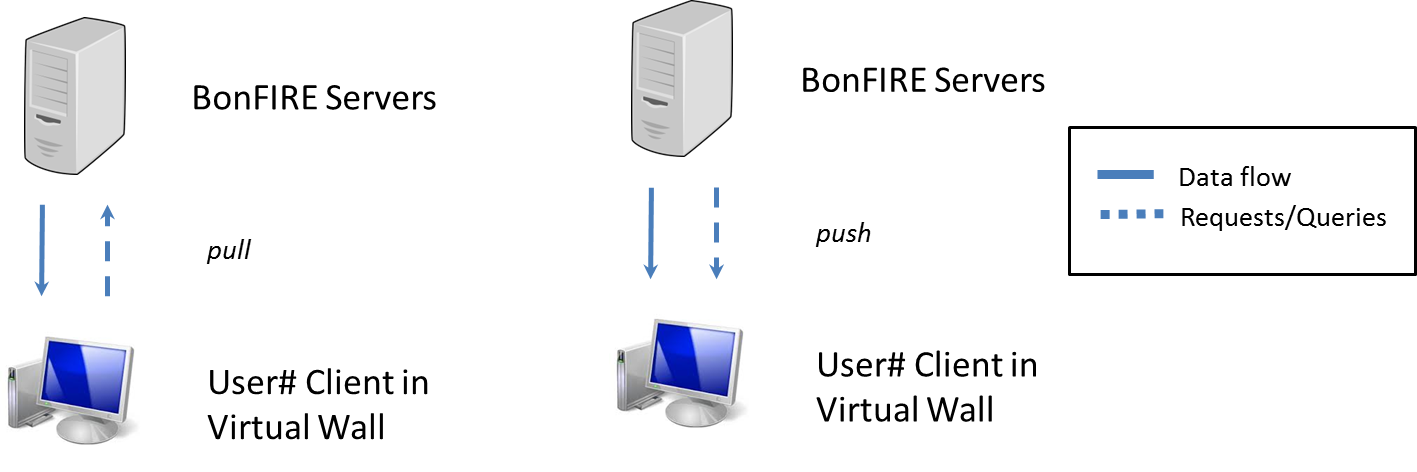
\includegraphics[width=6.3044in,height=2.10023in]{out-img44.png} \par}

{\centering\bfseries
\label{bkm:Ref378773360}Figure\ 36.\ Types of connectivity between
Virtual\ Wall Layer 3 and BonFIRE nodes.
\par}


\bigskip

In the virtual machines created in the VW nodes a script will emulate
different loads to simulate accesses to BonFIRE and transfer of data.


\bigskip

\paragraph[Design for the Scenario 1 Emergencies {}- Lorca Earthquake
(Spain)]{Design for the Scenario 1 Emergencies - Lorca Earthquake
(Spain)}

\bigskip

Resources and characteristics required for the deployment of the
scenario 1 in Virtual Wall:\ 

\liststyleLFOxl
\begin{itemize}
\item TBD nodes {\textgreater} 5
\item Connectivity\ HTTP\ and\ FTP
\item Pull type service (see\ Figure 36).
\item Bandwidth: different values for each node in the range of
1Mbps-1Gbps.
\item Latency, loss rate and background noise will be obtained from PLE
measurements.
\end{itemize}
\paragraph[Design for the Scenario 2 Infrastructure monitoring {}-
Affection in railway infrastructures by sand movement in desert areas
(Spain)]{Design for the Scenario 2 Infrastructure monitoring -
Affection in railway infrastructures by sand movement in desert areas
(Spain)}

\bigskip

Resources and characteristics required for the deployment of the
scenario 2 in Virtual Wall:\ 

\liststyleLFOxl
\begin{itemize}
\item 3 nodes
\item Connectivity\ HTTP
\item Pull type service (see\ Figure 36).
\item Bandwidth: different values for each node in the range of
1Mbps-1Gbps.
\item Latency, loss rate and background noise will be obtained from PLE
measurements.
\end{itemize}
In the virtual machines created in the VW nodes a script will emulate
different loads to simulate accesses to BonFIRE and transfer of data.


\bigskip

\paragraph[Design for the Scenario 3 Land Management {}-- South West of
England.]{Design for the Scenario 3 Land Management -- South West of
England.}

\bigskip

Resources and characteristics required for the deployment of the
scenario 3 in Virtual Wall:\ 

\liststyleLFOxl
\begin{itemize}
\item 1 node
\item Connectivity\ HTTP
\item Push type service (see\ Figure 36).
\item Bandwidth: different values for each node in the range of
1Mbps-1Gbps.
\item Latency, loss rate and background noise will be obtained from PLE
measurements.
\end{itemize}

\bigskip

\paragraph[Design for the Scenario 4 Precision Agriculture {}--
Argentina.]{Design for the Scenario 4 Precision Agriculture --
Argentina.}

\bigskip

Resources and characteristics required for the deployment of the
scenario 4 in Virtual Wall:\ 

\liststyleLFOxl
\begin{itemize}
\item 2 nodes
\item Connectivity\ HTTP\ for the push service (1 node),\ FTP\ for the
hosting (1 node).
\item Push type service 1 node (see\ Figure 36) and hosting with the
other node.
\item bandwidth: different values for each node in the range of
1Mbps-1Gbps.
\item Latency, loss rate and background noise will be obtained from PLE
measurements.
\end{itemize}
\paragraph[Design for the Scenario 5 Basemaps {}--\ Worldwide.]{Design
for the Scenario 5 Basemaps --\ Worldwide.}

\bigskip

Resources and characteristics required for the deployment of the
scenario 5 in Virtual Wall:\ 

\liststyleLFOxl
\begin{itemize}
\item n nodes {\textgreater} 10.
\item Connectivity\ HTTP
\item Pull type service (see\ Figure 36).
\item Bandwidth: different values for each node in the range of
1Mbps-1Gbps.
\item Latency, loss rate and background noise will be obtained from PLE
measurements.
\end{itemize}
\paragraph[Design for the Scenario 6 Online Catalogue / Ordering {}--
Worldwide.]{Design for the Scenario 6 Online Catalogue / Ordering --
Worldwide.}

\bigskip

Resources and characteristics required for the deployment of the
scenario 6 in Virtual Wall:\ 

\liststyleLFOxl
\begin{itemize}
\item 3 nodes.
\item Connectivity\ HTTP
\item Pull type service (see\ Figure 36).
\item Bandwidth: different values for each node in the range of
1Mbps-1Gbps.
\item Latency, loss rate and background noise will be obtained from PLE
measurements.
\end{itemize}

\bigskip

\subsection[Updating of the networks parameters]{Updating of the
networks parameters}
\hypertarget{Toc381777235}{}
\bigskip

The network parameters previously defined: latency, bandwidth,
background traffic and loss rate will be measured in real networks
implemented in PlanetLab Europe. After measuring them in that testbed,
they will be computed in the networks implemented in Virtual Wall.
See\ Figure 37.


\bigskip


\bigskip

{\centering 
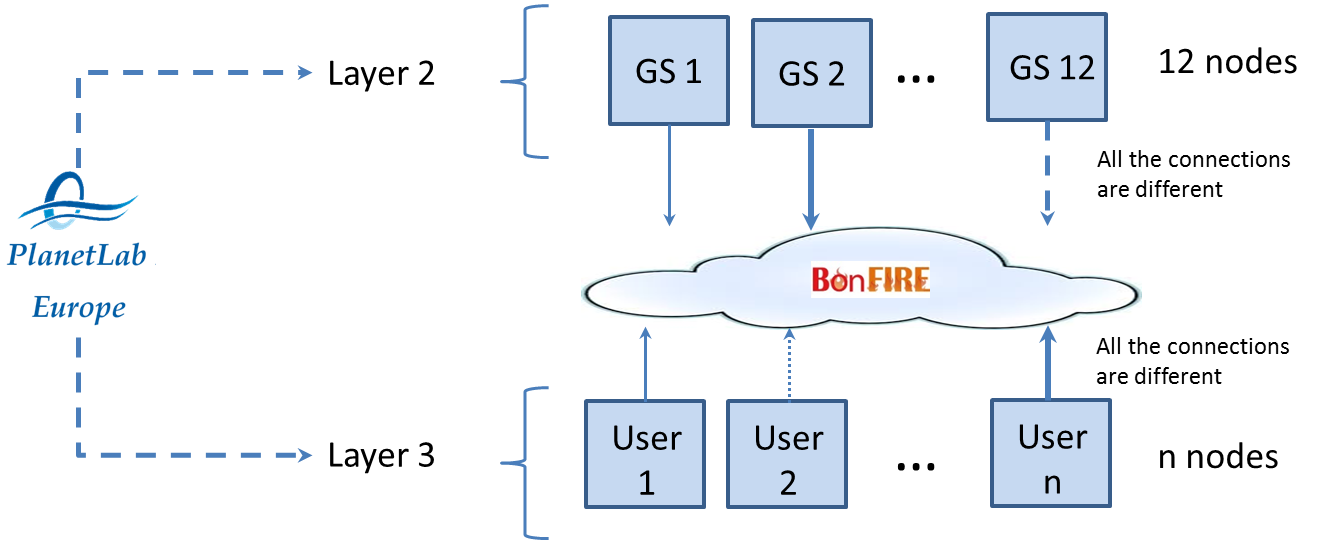
\includegraphics[width=6.18143in,height=2.50956in]{out-img45.png} \par}

{\centering\bfseries
\label{bkm:Ref378263310}Figure\ 37.\ Update of the networks parameters.
\par}


\bigskip

\subsection[Data, control and monitoring parameters]{Data, control and
monitoring parameters}
\hypertarget{Toc381777236}{}
\bigskip

\subsubsection[Data]{Data}
\hypertarget{Toc381777237}{}The data that will be transferred between
nodes. It will be images of about 2GB size.


\bigskip

\subsubsection[Control parameters]{Control parameters}
\hypertarget{Toc381777238}{}
\bigskip

The control parameters are depicted in the following table:


\bigskip

\begin{center}
\tablehead{}
\begin{supertabular}{|m{2.4677598in}|}
\hline
\centering\arraybslash \bfseries Virtual Wall control parameters\\\hline
\centering\arraybslash Bandwidth\\\hline
\centering\arraybslash Latency\\\hline
\centering\arraybslash Loss rate\\\hline
\centering\arraybslash Background noise\\\hline
\end{supertabular}
\end{center}

\bigskip

\subsubsection[Monitoring parameters]{Monitoring parameters}
\hypertarget{Toc381777239}{}
\bigskip

The monitoring parameters are the outputs to BonFIRE:


\bigskip

\begin{center}
\tablehead{}
\begin{supertabular}{|m{2.4677598in}|}
\hline
\centering\arraybslash \bfseries Virtual Wall monitoring
parameters\\\hline
\centering\arraybslash BonFIRE clients\\\hline
\centering\arraybslash BonFIRE servers\\\hline
\end{supertabular}
\end{center}

\bigskip

\subsection[Data flow and configuration of the nodes]{Data flow and
configuration of the nodes}
\hypertarget{Toc381777240}{}
\bigskip

The data flow is the following:

\liststyleLFOxxxv
\setcounter{saveenum}{\value{enumi}}
\begin{enumerate}
\setcounter{enumi}{\value{saveenum}}
\item The Sat\# servers store the images and execute the scripts that
emulate the GEO-Cloud satellites.
\item The GS\# clients request the data from the Sat\# servers and it is
retrieved.
\item The GS nodes act now as servers and the data is distributed to the
BonFIRE cloud. BonFIRE requests the data to the GS\# servers and it is
transferred.\ 
\item The User\# clients in Virtual Wall can be of two types:

\setcounter{saveenum}{\value{enumii}}
\begin{enumerate}
\setcounter{enumii}{\value{saveenum}}
\item The User\# client is pulling over the BonFIRE server to retrieve
the data.
\item The BonFIRE server (emulating a subscription) sends the data to
the User\# client.
\end{enumerate}
\end{enumerate}
Note: Just for clarification, some User\# nodes will do pulling, but
some others will get the data as if it was a subscription, i.e.,
BonFIRE will push the data to the User\# client.

See\ Figure 29\ for a graphical description of the data flow and
configuration of the nodes.


\bigskip


\bigskip

{\centering 
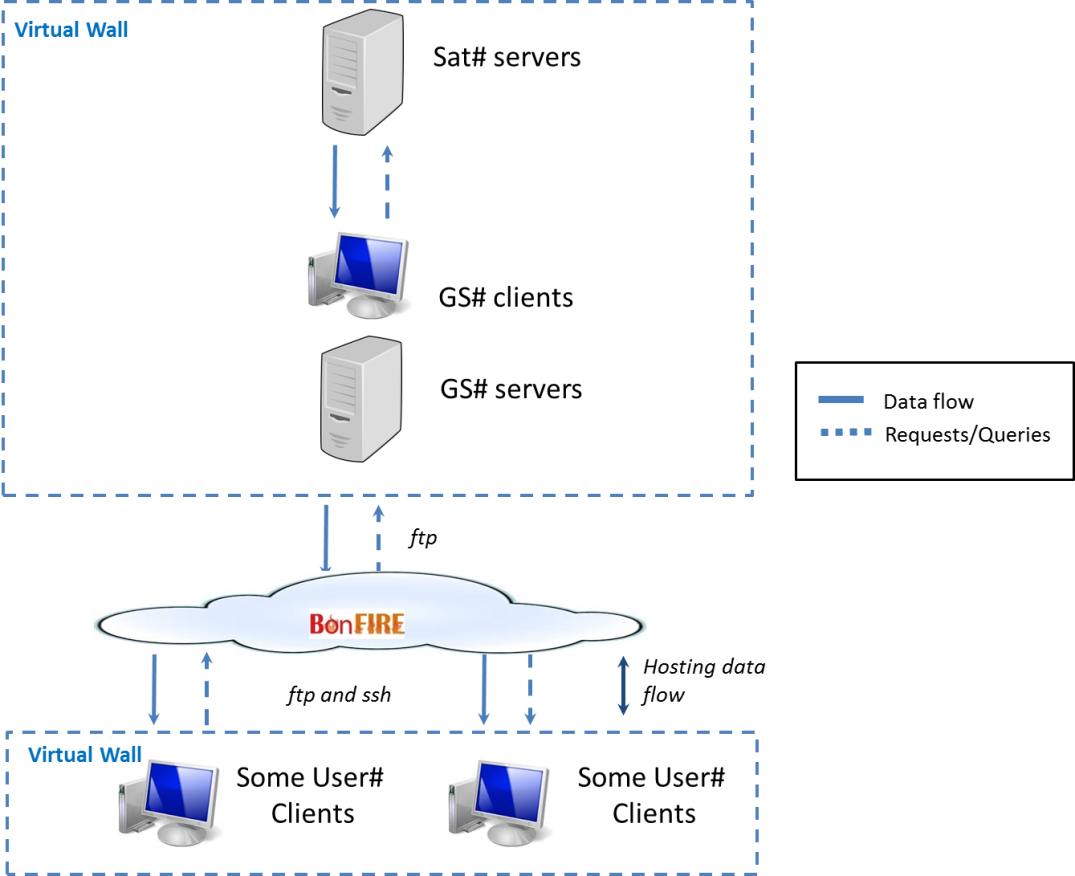
\includegraphics[width=4.8855in,height=3.98068in]{out-img46.png} \par}

{\centering\bfseries
Figure\ 38.\ Data flow and configuration of the nodes.
\par}


\bigskip

\subsection[Summary]{Summary}
\hypertarget{Toc381777241}{}
\bigskip

In this document the models to be implemented in Virtual Wall were
described and designed for its testing. The resources that will be used
for the experiment are defined so as to the connectivity between
required between Virtual Wall and BonFIRE.

\section[Network design in PlanetLab Europe]{Network design in PlanetLab
Europe}
\label{bkm:Ref378931923}\hypertarget{Toc381777242}{}
\bigskip

In this section the topology networks to be implemented in PlanetLab
Europe for the execution of the GEO-Cloud experiment are designed.\ 


\bigskip

In Planet Lab Europe two networks will be created:

\liststyleLFOxxxviii
\setcounter{saveenum}{\value{enumi}}
\begin{enumerate}
\setcounter{enumi}{\value{saveenum}}
\item Transferring data from different nodes representing ground
stations (GS) to one node representing a cloud node. The first approach
is pulling from the cloud node to the GS nodes.
\item Transferring data from a node representing a cloud node to
different nodes located around the world representing end users (user
node) accessing the cloud. Some of the user nodes will do pulling over
the cloud node, some others will receive pushing from the cloud node.
(TBD).\ 
\end{enumerate}
In the PLE networks created we intend to measure the following
impairments: latency, loss rate, background noise.\ 


\bigskip

In the PLE networks created we intend to control the bandwidth.\ 


\bigskip

The parameters measured and controlled in the PLE networks will be used
to update the parameters of the models implemented in Virtual Wall and
BonFIRE.


\bigskip

Figure 30\ depicts the relation between PlanetLab Europe and Virtual
Wall.


\bigskip


\bigskip

{\centering 
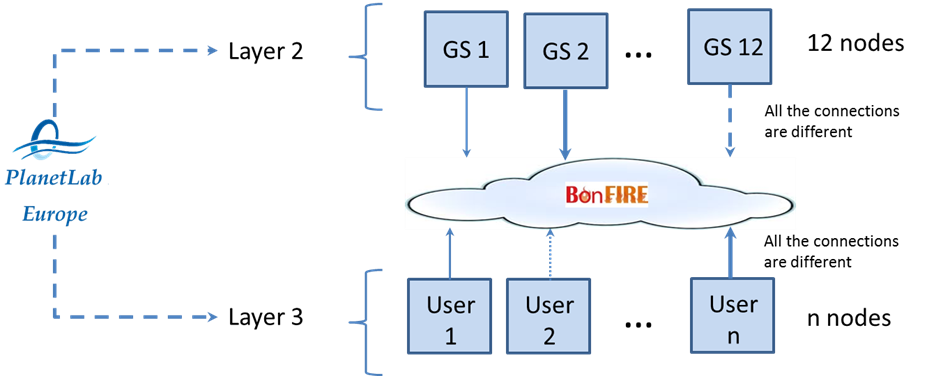
\includegraphics[width=5.45091in,height=2.21099in]{out-img47.png} \par}

{\centering\bfseries
Figure\ 39.\ Relation between PLE, VW and BF.
\par}

\subsection[Architecture]{Architecture}
\hypertarget{Toc381777243}{}
\bigskip

The system architecture is constituted of two layers:

\liststyleLFOxxxvi
\begin{itemize}
\item Layer 1: Network between ground stations and cloud. 12 nodes
located around the world are communicated with one server. The first
approach is that the server pulls over the different nodes to receive
data from them.
\item Layer 2: Network between cloud and end users. In this case a
single node emulating a cloud server is connected with different nodes
around the world emulating end users accessing the cloud. Some of the
nodes emulating end users will pull over the cloud node to receive
data. Some others will receive data from the cloud in a push way. \ The
number of nodes that will emulate end users are still TBD.
\end{itemize}

\bigskip

{\centering 
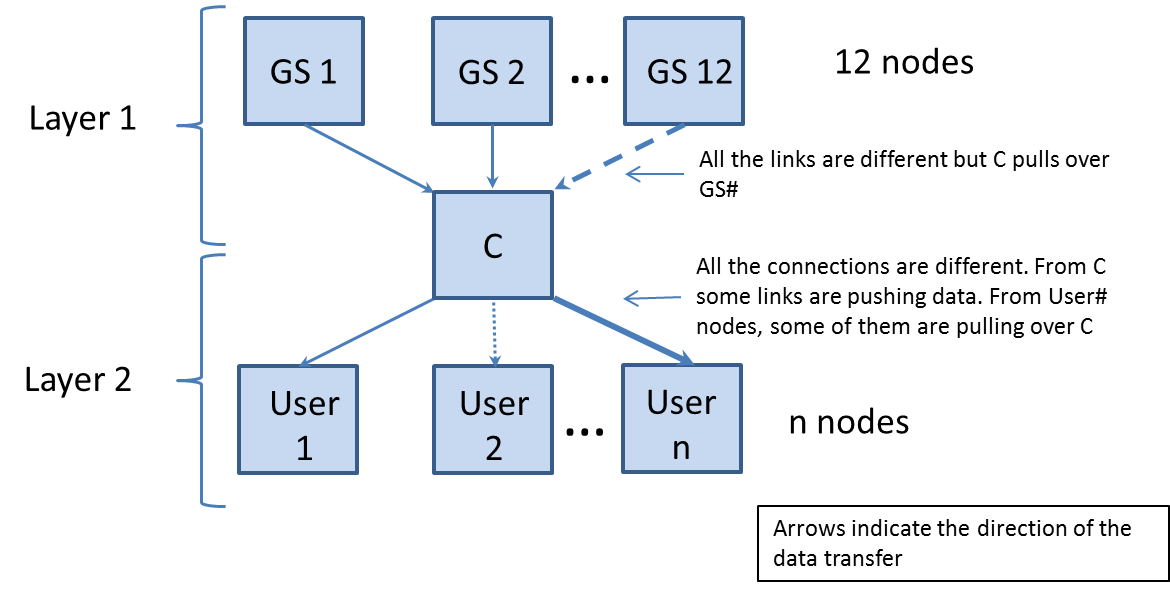
\includegraphics[width=5.26134in,height=2.6487in]{out-img48.png} \par}

{\centering\bfseries
Figure\ 40.\ GEO-Cloud architecture in PlanetLab Europe.
\par}


\bigskip


\bigskip

\subsection[Layer 1]{Layer 1}
\hypertarget{Toc381777244}{}
\bigskip

To constitute the layer 1 we need 12 GS nodes. In every node a script
will be computed to configure the node and manage the data that has to
be transferred to the C node.


\bigskip

Firstly, we define the nodes that will be used in PLE. They are based in
the real locations of the Ground Stations that will be emulated and the
BonFIRE cloud.


\bigskip


\bigskip

{\centering 
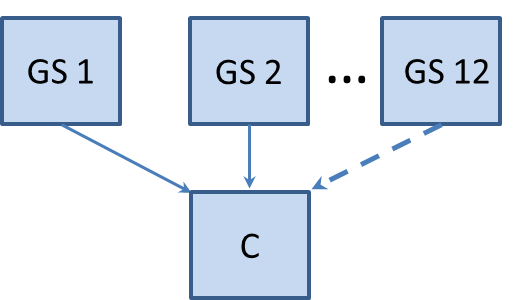
\includegraphics[width=2.36591in,height=1.38071in]{out-img49.png} \par}

{\centering\bfseries
Figure\ 41.\ Layer 1 network scheme.
\par}


\bigskip


\bigskip


\bigskip


\bigskip

The real ground stations are depicted in\ Table 6.


\bigskip


\bigskip

{\centering\bfseries
Table\ 17.\ Ground stations.
\par}

\begin{center}
\tablehead{}
\begin{supertabular}{m{1.6149598in}m{1.6149598in}}
\hline
\centering \bfseries\color{black} Ground Station &
\centering\arraybslash \bfseries\color{black} Location\\\hline
\centering \bfseries\color{black} Irkutsk &
\centering\arraybslash \color{black} Russia\\
\centering \bfseries\color{black} Puertollano &
\centering\arraybslash \color{black} Spain\\
\centering \bfseries\color{black} Svalbard\  &
\centering\arraybslash \color{black} Norway\\
\centering \bfseries\color{black} Troll\  &
\centering\arraybslash \color{black} Antarctic\ \\
\centering \bfseries\color{black} Chetumal &
\centering\arraybslash \color{black} Mexico\\
\centering \bfseries\color{black} Cordoba &
\centering\arraybslash \color{black} Argentina\\
\centering \bfseries\color{black} Dubai &
\centering\arraybslash \color{black} United Arab Emirates\\
\centering \bfseries\color{black} Kourou &
\centering\arraybslash \color{black} French Guiana\\
\centering \bfseries\color{black} Krugersdorp &
\centering\arraybslash \color{black} South Africa\\
\centering \bfseries\color{black} Malaysia &
\centering\arraybslash \color{black} Malaysia\\
\centering \bfseries\color{black} Prince Albert &
\centering\arraybslash \color{black} Canada\\\hline
\centering \bfseries\color{black} Sidney &
\centering\arraybslash \textcolor{black}{Australia}\\\hline
\end{supertabular}
\end{center}

\bigskip


\bigskip


\bigskip

In\ Figure 42\ the ideal location where could be the GS nodes are
depicted.


\bigskip

{\centering 
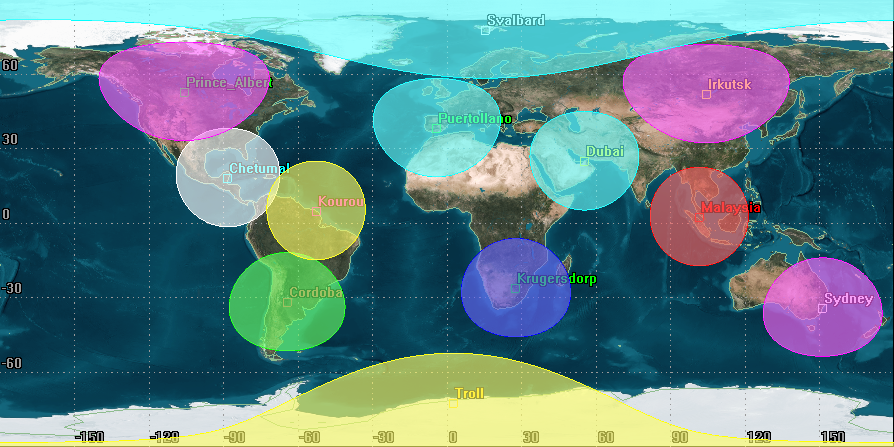
\includegraphics[width=6.29861in,height=3.14931in]{out-img50.png} \par}

{\centering\bfseries
\label{bkm:Ref378932776}Figure\ 42. Location of the GS nodes.
\par}


\bigskip


\bigskip


\bigskip


\bigskip


\bigskip


\bigskip

In the following table the GS nodes selected in PLE are depicted:


\bigskip

\begin{center}
\tablehead{\hline
\centering \bfseries\color{black} Node name &
\centering \bfseries\color{black} PLE node &
\centering \bfseries\color{black} Location &
\centering \bfseries\color{black} Test-bed &
\centering \bfseries\color{black} website &
\centering \bfseries\color{black} nodes &
\centering\arraybslash \bfseries\color{black} slices\\\hline}
\begin{supertabular}{|m{1.1989598in}|m{0.88435984in}|m{0.70875984in}|m{0.41355985in}|m{1.7149599in}|m{0.48995987in}|m{0.48645982in}|}
\centering \bfseries\color{black} GS-Irkutsk &
\centering \color{black} Beihang University &
\centering \color[rgb]{0.21176471,0.37254903,0.5686275} China &
\centering \color[rgb]{0.21176471,0.37254903,0.5686275} PLC &
\centering
\href{http://www.buaa.edu.cn/}{\textcolor[rgb]{0.43137255,0.6156863,0.06666667}{http://www.buaa.edu.cn}}
&
\centering \color{black} 2 &
\centering\arraybslash \color{black} 2\\\hline
\centering \bfseries\color{black} GS-Puertollano &
\centering \color{black} Universidad Carlos III Madrid &
\centering \color[rgb]{0.21176471,0.37254903,0.5686275} Spain &
\centering \color[rgb]{0.21176471,0.37254903,0.5686275} PLE &
\centering
\href{http://www.planet-lab.eu/www.evalues.es}{\textcolor[rgb]{0.43137255,0.6156863,0.06666667}{www.evalues.es}}
&
\centering \color{black} 2 &
\centering\arraybslash \color{black} 0\\\hline
\centering \bfseries\color{black} GS-Svalbard &
\centering \color{black} University of Tromso &
\centering \color[rgb]{0.21176471,0.37254903,0.5686275} Norway &
\centering \color[rgb]{0.21176471,0.37254903,0.5686275} PLE &
\centering
\href{http://www.cs.uit.no/}{\textcolor[rgb]{0.43137255,0.6156863,0.06666667}{http://www.cs.uit.no}}
&
\centering \color[rgb]{0.21176471,0.37254903,0.5686275} 2 &
\centering\arraybslash \color[rgb]{0.21176471,0.37254903,0.5686275}
0\\\hline
\centering \bfseries\color{black} GS-Troll &
\centering \color{black} PlanetLab Colo - CLARA Santiago &
\centering \color[rgb]{0.21176471,0.37254903,0.5686275} Chile &
\centering \color[rgb]{0.21176471,0.37254903,0.5686275} PLC &
\centering \color{black} {}- &
\centering \color[rgb]{0.21176471,0.37254903,0.5686275} 2 &
\centering\arraybslash \color[rgb]{0.21176471,0.37254903,0.5686275}
0\\\hline
\centering \bfseries\color{black} GS-Chetumal &
\centering \color{black} University of Puerto Rico at Mayaguez &
\centering \color[rgb]{0.21176471,0.37254903,0.5686275} Puerto Rico &
\centering \color[rgb]{0.21176471,0.37254903,0.5686275} PLC &
\centering
\href{http://ece.uprm.edu/}{\textcolor[rgb]{0.43137255,0.6156863,0.06666667}{http://ece.uprm.edu}}
&
\centering \color[rgb]{0.21176471,0.37254903,0.5686275} 2 &
\centering\arraybslash \color[rgb]{0.21176471,0.37254903,0.5686275}
0\\\hline
\centering \bfseries\color{black} GS-Cordoba &
\centering \selectlanguage{spanish}\color{black} Instituto Tecnologico
Buenos Aires &
\centering \color[rgb]{0.21176471,0.37254903,0.5686275} Argentina &
\centering \color[rgb]{0.21176471,0.37254903,0.5686275} PLC &
\centering \url{http://www.itba.edu.ar/} &
\centering \color[rgb]{0.21176471,0.37254903,0.5686275} 2 &
\centering\arraybslash \color[rgb]{0.21176471,0.37254903,0.5686275}
0\\\hline
\centering \bfseries\color{black} GS-Dubai &
\centering \color{black} The Hebrew University of Jerusalem &
\centering \color[rgb]{0.21176471,0.37254903,0.5686275} Israel &
\centering \color[rgb]{0.21176471,0.37254903,0.5686275} PLE &
\centering \url{http://www.cs.huji.ac.il/labs/danss} &
\centering \color[rgb]{0.21176471,0.37254903,0.5686275} 2 &
\centering\arraybslash \color[rgb]{0.21176471,0.37254903,0.5686275}
0\\\hline
\centering \bfseries\color{black} GS-Kourou &
\centering \color{black} RNP &
\centering \color[rgb]{0.21176471,0.37254903,0.5686275} Brazil &
\centering \color[rgb]{0.21176471,0.37254903,0.5686275} PLC &
\centering
\href{http://rnp.br/}{\textcolor[rgb]{0.43137255,0.6156863,0.06666667}{http://rnp.br}}
&
\centering \color[rgb]{0.21176471,0.37254903,0.5686275} 2 &
\centering\arraybslash \color[rgb]{0.21176471,0.37254903,0.5686275}
0\\\hline
\centering \bfseries\color{black} GS-Krugersdorp &
\centering \color{black} Universite de La Reunion &
\centering \color[rgb]{0.21176471,0.37254903,0.5686275} Reunion Island
(France) &
\centering \color[rgb]{0.21176471,0.37254903,0.5686275} PLE &
\centering
\href{http://lim.univ-reunion.fr/}{\textcolor[rgb]{0.43137255,0.6156863,0.06666667}{http://lim.univ-reunion.fr}}
&
\centering \color[rgb]{0.21176471,0.37254903,0.5686275} 2 &
\centering\arraybslash \color[rgb]{0.21176471,0.37254903,0.5686275}
0\\\hline
\centering \bfseries\color{black} GS-Malaysia &
\centering \color{black} National University of Singapore &
\centering \color[rgb]{0.21176471,0.37254903,0.5686275} Malaysia &
\centering \color[rgb]{0.21176471,0.37254903,0.5686275} PLC &
\centering
\href{http://www.comp.nus.edu.sg/}{\textcolor[rgb]{0.43137255,0.6156863,0.06666667}{http://www.comp.nus.edu.sg}}
&
\centering \color[rgb]{0.21176471,0.37254903,0.5686275} 3 &
\centering\arraybslash \color[rgb]{0.21176471,0.37254903,0.5686275}
3\\\hline
\centering \bfseries\color{black} GS-Prince Albert &
\centering \color{black} University of Saskatchewan &
\centering \color[rgb]{0.21176471,0.37254903,0.5686275} Canada &
\centering \color[rgb]{0.21176471,0.37254903,0.5686275} PLC &
\centering
\href{http://usask.ca/}{\textcolor[rgb]{0.43137255,0.6156863,0.06666667}{http://usask.ca}}
&
\centering \color[rgb]{0.21176471,0.37254903,0.5686275} 2 &
\centering\arraybslash \color[rgb]{0.21176471,0.37254903,0.5686275}
0\\\hline
\centering \bfseries\color{black} GS-Sidney &
\centering \textcolor{black}{National ICT Australia} &
\centering \textcolor[rgb]{0.21176471,0.37254903,0.5686275}{Australia} &
\centering \textcolor[rgb]{0.21176471,0.37254903,0.5686275}{PLE} &
\centering
\href{http://www.nicta.com.au/}{\textcolor[rgb]{0.43137255,0.6156863,0.06666667}{http://www.nicta.com.au}}
&
\centering \textcolor[rgb]{0.21176471,0.37254903,0.5686275}{2} &
\centering\arraybslash
\textcolor[rgb]{0.21176471,0.37254903,0.5686275}{5}\\\hline
\end{supertabular}
\end{center}

\bigskip

Some of the previous nodes are not in the same location of the
real\ ground stations. We selected a\ node near the specific ground
station.


\bigskip


\bigskip


\bigskip


\bigskip


\bigskip


\bigskip


\bigskip


\bigskip


\bigskip

The C node will be the following:


\bigskip

\begin{center}
\tablehead{}
\begin{supertabular}{|m{1.1774598in}|m{0.90595984in}|m{0.70875984in}|m{0.41355985in}|m{1.6927599in}|m{0.5121598in}|m{0.48645982in}|}
\hline
\centering \bfseries Node Name &
\centering \bfseries\color{black} node &
\centering \bfseries\color{black} Location &
\centering \bfseries\color{black} Test-bed &
\centering \bfseries\color{black} website &
\centering \bfseries\color{black} nodes &
\centering\arraybslash \bfseries\color{black} slices\\\hline
\centering Cloud &
\centering {\color{black} Universite Pierre et Marie Curie}\par

~
 &
\centering France &
\centering PLE &
\centering
\href{http://www.lip6.fr/}{\textcolor[rgb]{0.43137255,0.6156863,0.06666667}{http://www.lip6.fr}}
&
\centering 10 &
\centering\arraybslash 15\\\hline
\end{supertabular}
\end{center}

\bigskip


\bigskip

The communications between nodes in the Layer 1 in PLE are of pull type
through\ FTP\ if possible (HTTP\ or\ SSH\ otherwise), i.e, the C client
requests retrieving the data from the GS\# nodes, see the following
figure:


\bigskip

{\centering 
\includegraphics[width=3.66899in,height=1.94574in]{out-img51.png} \par}


\bigskip

{\centering\bfseries
Figure\ 43.\ Types of connectivity between PLE nodes in Layer 1.
\par}


\bigskip

\subsection[Layer 2]{Layer 2}
\hypertarget{Toc381777245}{}
\bigskip

The scheme of the Layer 2 is depicted in the following picture:


\bigskip

{\centering 
\includegraphics[width=3.07447in,height=1.37611in]{out-img52.png} \par}

{\centering\bfseries
Figure\ 44. Layer 2 network scheme.
\par}


\bigskip


\bigskip


\bigskip


\bigskip


\bigskip

The C node is the same of the previous case:


\bigskip

\begin{center}
\tablehead{}
\begin{supertabular}{|m{1.1774598in}|m{0.90595984in}|m{0.70875984in}|m{0.41355985in}|m{1.6927599in}|m{0.5121598in}|m{0.48645982in}|}
\hline
\centering \bfseries Node Name &
\centering \bfseries\color{black} node &
\centering \bfseries\color{black} Location &
\centering \bfseries\color{black} Test-bed &
\centering \bfseries\color{black} website &
\centering \bfseries\color{black} nodes &
\centering\arraybslash \bfseries\color{black} slices\\\hline
\centering Cloud &
\centering {\color{black} Universite Pierre et Marie Curie}\par

~
 &
\centering France &
\centering PLE &
\centering
\href{http://www.lip6.fr/}{\textcolor[rgb]{0.43137255,0.6156863,0.06666667}{http://www.lip6.fr}}
&
\centering 10 &
\centering\arraybslash 15\\\hline
\end{supertabular}
\end{center}

\bigskip

The User\# nodes will be selected for the scenarios proposed
in\ Section\ 3:

\liststyleLFOxxxix
\setcounter{saveenum}{\value{enumi}}
\begin{enumerate}
\setcounter{enumi}{\value{saveenum}}
\item Scenario 1: Emergencies - Lorca Earthquake (Spain)
\item Scenario 2: Infrastructure monitoring - Affection in railway
infrastructures by sand movement in desert areas (Spain)
\item Scenario 3: Land Management -- South West of England.
\item Scenario 4: Precision Agriculture -- Argentina.
\item Scenario 5: Basemaps --\ Worldwide.
\item Scenario 6: Online Catalogue / Ordering -- Worldwide.
\end{enumerate}
Although during the implementation stage we will evaluate the
possibility of including new scenarios for testing.


\bigskip

Because we will use NEPI for the provisioning of nodes we will not fix
the nodes as done in the previous cases for the GS\# and C nodes, we
will indicate the country attribute and NEPI will automatically select
the available node in that country.


\bigskip

The communications between nodes in the Layer 2 in PLE can be of two
types: pull and push, both through\ HTTP, see next figure:

{\centering 
\includegraphics[width=6.18082in,height=2.02427in]{out-img53.png} \par}

{\centering\bfseries
Figure\ 45.\ Types of connectivity between PLE\ nodes in Layer 2.
\par}


\bigskip

The characteristics and number of nodes selected for each scenario are
described as follows.

\subsubsection[Design for the Scenario 1 Emergencies {}- Lorca
Earthquake (Spain)]{Design for the Scenario 1 Emergencies - Lorca
Earthquake (Spain)}
\hypertarget{Toc381777246}{}
\bigskip

Resources and characteristics required for the deployment of the
scenario 1 in PLE:\ 

\liststyleLFOxl
\begin{itemize}
\item TBD nodes {\textgreater} 5
\item Pull type service (see\ Figure 36).
\item Countries: Spain, France, UK.\ 
\end{itemize}
\subsubsection[Design for the Scenario 2 Infrastructure monitoring {}-
Affection in railway infrastructures by sand movement in desert areas
(Spain)]{Design for the Scenario 2 Infrastructure monitoring -
Affection in railway infrastructures by sand movement in desert areas
(Spain)}
\hypertarget{Toc381777247}{}
\bigskip

Resources and characteristics required for the deployment of the
scenario 2 in PLE:\ 

\liststyleLFOxl
\begin{itemize}
\item 3 nodes
\item Pull type service (see\ Figure 36).
\item Countries: Spain, Italy, Germany.
\end{itemize}
\subsubsection[Design for the Scenario 3 Land Management {}-- South West
of England.]{Design for the Scenario 3 Land Management -- South West of
England.}
\hypertarget{Toc381777248}{}
\bigskip

Resources and characteristics required for the deployment of the
scenario 3 in PLE:\ 

\liststyleLFOxl
\begin{itemize}
\item 1 node.
\item Push type service (see\ Figure 36).
\item Countries: UK.
\end{itemize}
\subsubsection[Design for the Scenario 4 Precision Agriculture {}--
Argentina.]{Design for the Scenario 4 Precision Agriculture --
Argentina.}
\hypertarget{Toc381777249}{}
\bigskip

Resources and characteristics required for the deployment of the
scenario 4 in PLE:\ 

\liststyleLFOxl
\begin{itemize}
\item 2 nodes
\item Push type service 1 node (see\ Figure 36) and push for hosting in
other node.
\item Countries: Argentina.
\end{itemize}
\subsubsection[Design for the Scenario 5 Basemaps
{}--\ Worldwide.]{Design for the Scenario 5 Basemaps --\ Worldwide.}
\hypertarget{Toc381777250}{}
\bigskip

Resources and characteristics required for the deployment of the
scenario 5 in PLE:\ 

\liststyleLFOxl
\begin{itemize}
\item n nodes {\textgreater} 10 (TBD).
\item Pull type service (see\ Figure 36).
\item Countries: Worldwide.
\end{itemize}
\subsubsection[Design for the Scenario 6 Online Catalogue / Ordering
{}-- Worldwide.]{Design for the Scenario 6 Online Catalogue / Ordering
-- Worldwide.}
\hypertarget{Toc381777251}{}
\bigskip

Resources and characteristics required for the deployment of the
scenario 6 in PLE:\ 

\liststyleLFOxl
\begin{itemize}
\item 3 nodes.
\item Pull type service (see\ Figure 36).
\item Countries: (Australia, USA, Iceland).
\end{itemize}

\bigskip

\subsection[Data, control and monitoring parameters]{Data, control and
monitoring parameters}
\hypertarget{Toc381777252}{}
\bigskip

\subsubsection[Data]{Data}
\hypertarget{Toc381777253}{}The data that has to be transferred between
nodes will be images of about 2GB size.


\bigskip

\subsubsection[Control parameters]{Control parameters}
\hypertarget{Toc381777254}{}
\bigskip

The parameter that we intend to control is the Bandwidth of the
networks.


\bigskip

\begin{center}
\tablehead{}
\begin{supertabular}{|m{2.4677598in}|}
\hline
\centering\arraybslash \bfseries PLE control parameters\\\hline
\centering\arraybslash Bandwidth\\\hline
\end{supertabular}
\end{center}

\bigskip


\bigskip

\subsubsection[Monitoring parameters]{Monitoring parameters}
\hypertarget{Toc381777255}{}
\bigskip

The monitoring parameters are depicted in the following table:


\bigskip

\begin{center}
\tablehead{}
\begin{supertabular}{|m{2.4677598in}|}
\hline
\centering\arraybslash \bfseries PLE monitoring parameters\\\hline
\centering\arraybslash Latency\\\hline
\centering\arraybslash Loss Rate\\\hline
\centering\arraybslash Background noise\\\hline
\end{supertabular}
\end{center}

\bigskip

\subsection[Data flow and configuration of the nodes]{Data flow and
configuration of the nodes}
\hypertarget{Toc381777256}{}
\bigskip

The data flow is the following:

\liststyleLFOxxxv
\setcounter{saveenum}{\value{enumi}}
\begin{enumerate}
\setcounter{enumi}{\value{saveenum}}
\item The GS servers have the data that has to be transferred to the
{\textquotedblleft}Cloud{\textquotedblright} (C) node (cloud is the
name of the node as previously defined). The C node can act as a client
to the GS servers and as Servers to the User clients.
\item The C client requests the GS server to retrieve the data and the
data is transferred from GS\# to C.
\item The data is transferred from the Cloud node to the User\# clients.
There are two options.

\setcounter{saveenum}{\value{enumii}}
\begin{enumerate}
\setcounter{enumii}{\value{saveenum}}
\item The User\# client is pulling over the Cloud server to retrieve the
data.
\item The Cloud server (emulating a subscription) sends the data to the
User\# client.
\end{enumerate}
\end{enumerate}
Note: Just for clarification, some User\# nodes will do pulling, but
some others will get the data as if it was a subscription, i.e., the C
node will push the data to the User\# client.

See\ Figure 29\ for a graphical description of the data flow and
configuration of the nodes.


\bigskip

{\centering 
\includegraphics[width=5.38135in,height=2.87144in]{out-img54.png} \par}

{\centering\bfseries
Figure\ 46.\ Data flow and configuration of the nodes.
\par}

\subsection[Summary]{Summary}
\hypertarget{Toc381777257}{}In this document the design of the
experiment that will be implemented in PlanetLab Europe is defined. The
resources that will be used during the implementation and
experimentation were also described so as to the parameters for control
and monitoring.\ 

\section[Bibliography]{Bibliography}
\hypertarget{Toc381777258}{}\label{bkm:Ref378931932}
\bigskip

Amundsen, B{\aa}rd and Thomas Keilman. {\textquotedbl}Natural disasters
-- is your municipality vulnerable?{\textquotedbl}\ \textit{Natural
disasters -- is your municipality vulnerable?}\ March 2013.
{\textless}http://www.forskningsradet.no/en/Newsarticle/Natural\_disasters\_\_is\_your\_municipality\_vulnerable/1253984593679?lang=en{\textgreater}.

Astrium. {\textquotedbl}Precision
Agriculture.{\textquotedbl}\ \textit{Precision Agriculture}. 2013.
{\textless}http://www.astrium-geo.com/en/1003-precision-agriculture{\textgreater}.

Commission, European. {\textquotedbl}Examining the creation of a
European Border Surveillance System
(EUROSUR).{\textquotedbl}\ \textit{Examining the creation of a European
Border Surveillance System (EUROSUR)}. February 2008.
{\textless}http://eur-lex.europa.eu/LexUriServ/LexUriServ.do?uri=COM:2008:0068:FIN:EN:PDF{\textgreater}.

Corbane, Christina, et al. {\textquotedbl}A complete processing chain
for ship detection using optical satellite
imagery.{\textquotedbl}\ \textit{International Journal of Remote
Sensing}. Taylor {\textbackslash}\& Francis, 2010. 5837--5854.
{\textless}http://dl.acm.org/citation.cfm?id=1898618{\textgreater}.

Gardner, Frank. {\textquotedbl}Seeking Somali pirates, from the
air.{\textquotedbl}\ \textit{Seeking Somali pirates, from the air}.
February 2012.
{\textless}http://www.bbc.co.uk/news/world-middle-east-17095887{\textgreater}.

Hot.\ \textit{Imagery for Haiyan}. 17 December 2013.
{\textless}http://hot.openstreetmap.org/updates/2013-12-17\_imagery\_for\_haiyan{\textgreater}.

\foreignlanguage{spanish}{Instituto Geogr\'afico Nacional, Universidad
Complutense de Madrid, Universidad Polit\'ecnica de Madrid Instituto
Geol\'ogico y Minero de Espa\~na Asociaci\'on Espa\~nola de
Ingenier\'ia S\'ismica. {\textquotedbl}Informe del sismo de Lorca del
11 de mayo de
2011.{\textquotedbl}\ }\foreignlanguage{spanish}{\textit{Informe del
sismo de Lorca del 11 de mayo de
2011}}\foreignlanguage{spanish}{.\ }July 2011.
{\textless}http://www.ign.es/ign/resources/sismologia/Lorca.pdf{\textgreater}.

Lakshmi, Venkat. {\textquotedbl}Use of Satellite Remote Sensing in
hydrological predictions in ungaged
basins.{\textquotedbl}\ \textit{Hydrological Processes}. 2004.
1029--1034.
{\textless}http://www.isprs.org/proceedings/XXXV/congress/comm1/papers/58.pdf{\textgreater}.

Miller, Steven D., Thomas F. Lee and Robert L. Fennimore.
{\textquotedbl}Satellite-Based Imagery Techniques for Daytime
Cloud/Snow Delineation from MODIS.{\textquotedbl}\ \textit{Journal of
Applied Meteorology}. American Meteorological Society, 2005. 987-997.
{\textless}http://journals.ametsoc.org/doi/pdf/10.1175/JAM2252.1{\textgreater}.

Sandau, Rainer. {\textquotedbl}Satellite Earth Observation and
Surveillance Payloads.{\textquotedbl}\ \textit{Systems Concepts and
Integration Panel}. Ed. NATO. 2009. 16p.
{\textless}https://www.cso.nato.int/pubs/rdp.asp?RDP=RTO-EN-SCI-209{\textgreater}.

Sensyf. {\textquotedbl}Services.{\textquotedbl}\ \textit{Services}.
2013. {\textless}http://www.sensyf.eu/services.html{\textgreater}.

Skaugen, Thomas. {\textquotedbl}Assimilating satellite derived snow
covered area (SCA) in hydrological
models.{\textquotedbl}\ \textit{Assimilating satellite derived snow
covered area (SCA) in hydrological models}. 2014.
{\textless}http://undine.bafg.de/servlet/is/15801/{\textgreater}.


\bigskip


\bigskip

\clearpage
\bigskip

\section[Appendix:\ Other scenarios]{Appendix:\ Other scenarios}
\label{bkm:Ref378852215}\hypertarget{Toc381777259}{}\subsection[Scenario\ 7:\ Maritime
surveillance {}-- Alboran Sea]{\selectlanguage{spanish}
Scenario\ 7:\ Maritime surveillance -- Alboran Sea}
\hypertarget{Toc381777260}{}\subsubsection[Scenario
description]{\selectlanguage{spanish} Scenario description}
\hypertarget{Toc381777261}{}
\bigskip

\foreignlanguage{english}{The Guardia Civil in Spain is working with
Frontex and the European Commission to implement the European Border
Surveillance System (EUROSUR)\ }(Commission)\foreignlanguage{english}{,
see\ }Figure 47\foreignlanguage{english}{. A critical area of the
European Frontiers is the Alboran Sea in the south of Spain. In this
area thousands of migrants lose their lives try to access the European
land from the African coasts.}


\bigskip

{\selectlanguage{english}
The Guardia Civil needs daily satellite imagery to detect immigration
activity in the emission costs in Africa to start the protocols of the
Spanish Maritime Rescue Agency to rescue the migrants{\textquoteright}
boats in the Alboran Sea.}


\bigskip

{\centering 
\includegraphics[width=4.04209in,height=2.62667in]{out-img55.png} \par}

{\centering\bfseries
\label{bkm:Ref377552833}Figure\ 47.\ Eurosur scheme.
\par}


\bigskip

\subsubsection[Response]{Response}
\hypertarget{Toc381777262}{}
\bigskip

{\selectlanguage{english}
The\ solicited\ service\ is based on the following premises:}

\liststyleLFOvii
\begin{itemize}
\item {\selectlanguage{english}
Permanent\ coverage\ }
\item {\selectlanguage{english}
Daily revisit time}
\item {\selectlanguage{english}
Urgent images}
\item {\selectlanguage{english}
The images of Alboran Sea\ should be\ distributed to the users through a
push type service.}
\item {\selectlanguage{english}
The images require an analysis to identify if there is immigrants
activity in the African coast. The analysis consists of
probabilistically identifying if there are trucks and dinghies in the
beaches.}
\end{itemize}

\bigskip

\subsubsection[Data distribution]{\selectlanguage{spanish} Data
distribution}
\hypertarget{Toc381777263}{}{\selectlanguage{spanish}
To be defined.}

\subsubsection[Area of Interest\ ]{\selectlanguage{english} Area of
Interest\ }
\hypertarget{Toc381777264}{}\foreignlanguage{english}{The Area of
Interest is the Alboran Sea in the south of Spain, see\ }Figure
48\foreignlanguage{english}{.}


\bigskip

{\centering 
\includegraphics[width=2.76092in,height=2.82543in]{out-img56.png} \par}

{\centering\bfseries
\label{bkm:Ref377554444}Figure\ 48.\ Alboran Sea Location (image
from\ http://upload.wikimedia.org).
\par}

\subsubsection[Users]{\selectlanguage{english} Users}
\hypertarget{Toc381777265}{}{\selectlanguage{english}
The users are Guardia Civil, Maritime Rescue Agency and the European
Commission.}

\subsubsection[Service Type]{\selectlanguage{english} Service Type}
\hypertarget{Toc381777266}{}{\selectlanguage{english}
The service type is high added value of a push type.\ }

\subsubsection[Processing Level]{\selectlanguage{english} Processing
Level}
\hypertarget{Toc381777267}{}{\selectlanguage{english}
The processing level is low.}

\subsubsection[Storage Level]{\selectlanguage{english} Storage Level}
\hypertarget{Toc381777268}{}{\selectlanguage{english}
The storage level is high, since images of the Alboran Sea have to be
daily recorded and stored.}

\subsubsection[Communications Level]{\selectlanguage{english}
Communications Level}
\hypertarget{Toc381777269}{}{\selectlanguage{english}
The communication level is urgent.}

\subsubsection[Demand Variability]{\selectlanguage{english} Demand
Variability}
\hypertarget{Toc381777270}{}\foreignlanguage{english}{The demand
variability is constant. See\ }Table 18\foreignlanguage{english}{\ for
a summary of the service characteristics.}


\bigskip

\clearpage{\centering\bfseries
Table\ 18.\ Relation of the users demand with the service offered in the
Scenario 7. In orange the characteristics of the service.
\par}

\begin{center}
\tablehead{}
\begin{supertabular}{m{0.22605985in}m{0.92955977in}m{0.68855983in}|m{1.0649599in}m{1.1274599in}|m{0.6718598in}m{0.21425986in}}
\hhline{~-----~}
\multicolumn{1}{m{0.22605985in}|}{~
} &
\multicolumn{2}{m{1.6968598in}|}{\centering \bfseries\color{black}
Service Type} &
\multicolumn{2}{m{2.27116in}|}{\centering \bfseries\color{black} Loads
in Cloud Technology} &
\multicolumn{1}{m{0.6718598in}|}{\bfseries\color{black} Demand
Variability} &
~
\\\hline
\multicolumn{1}{|m{0.22605985in}|}{\centering \bfseries\color{black}
COMPANY{\textquotesingle}S SERVICES} &
\multicolumn{1}{m{0.92955977in}|}{\centering \color{black} Basic} &
\centering \color{black} Basic &
\multicolumn{1}{m{1.0649599in}|}{\centering \color{black} Processing} &
\centering \color{black} Low &
\multicolumn{1}{m{0.6718598in}|}{\centering \color{black} Constant} &
\multicolumn{1}{m{0.21425986in}|}{\centering\arraybslash
\textbf{\textcolor{black}{USERS{\textquotesingle}
DEMA}}\foreignlanguage{spanish}{\textbf{\textcolor{black}{ND}}}}\\\hline
 &
 &
 &
 &
\centering \selectlanguage{spanish}\color{black} Medium &
 &
\\\hhline{~~~~-~~}
 &
 &
\centering \selectlanguage{spanish}\color{black} Advanced &
 &
\centering \selectlanguage{spanish}\color{black} High &
 &
\\\hhline{~~-~-~~}
 &
 &
 &
\multicolumn{1}{m{1.0649599in}|}{\centering
\selectlanguage{spanish}\color{black} Storage} &
\centering \selectlanguage{spanish}\color{black} Low &
\multicolumn{1}{m{0.6718598in}|}{\centering
\selectlanguage{spanish}\color{black} Variable} &
\\\hhline{~~~---~}
 &
\multicolumn{1}{m{0.92955977in}|}{\centering
\selectlanguage{spanish}\color{black} High added value} &
\centering \selectlanguage{spanish}\color{black} Pull\  &
 &
\centering \selectlanguage{spanish}\color{black} Medium &
 &
\\\hhline{~~-~-~~}
 &
 &
 &
 &
\centering \selectlanguage{spanish}\color{black} High &
 &
\\\hhline{~~~~-~~}
 &
 &
\centering \selectlanguage{spanish}\color{black} Push\  &
\multicolumn{1}{m{1.0649599in}|}{\centering
\selectlanguage{spanish}\color{black} Communications} &
\centering \selectlanguage{spanish}\color{black} Not urgent &
\multicolumn{1}{m{0.6718598in}|}{\centering
\selectlanguage{spanish}\color{black} Highly variable} &
\\\hhline{~~~---~}
 &
 &
 &
 &
\centering {\selectlanguage{spanish}\color{black} Urgent}\par

~
 &
 &
\\\hhline{~--~-~~}
 &
\multicolumn{2}{m{1.6968598in}|}{\centering
\selectlanguage{spanish}\color{black} Hosting} &
 &
 &
 &
\\\hhline{~--~~~~}
\end{supertabular}
\end{center}

\bigskip


\bigskip

\clearpage
\bigskip

\subsection[Scenario 8: \ Homeland Security {}- Lisbon]{Scenario 8:
\ Homeland Security - Lisbon}
\hypertarget{Toc381777271}{}\subsubsection[Scenario
description]{Scenario description}
\hypertarget{Toc381777272}{}\foreignlanguage{english}{Portugal
Government and Lisbon City Council\ }\foreignlanguage{english}{are
looking
to~}\href{http://www.satimagingcorp.com/services.html}{\foreignlanguage{english}{remote
sensing}}\foreignlanguage{english}{~and~}\href{http://www.satimagingcorp.com/svc/gismapping.html}{\foreignlanguage{english}{GIS}}\foreignlanguage{english}{~to
support\ }\foreignlanguage{english}{a security initiative for the city
of Lisbon\ }\foreignlanguage{english}{for both strategic planning and
for actual tactical deployment during a
disaster}\foreignlanguage{english}{, see\ }Figure
49\foreignlanguage{english}{.}\foreignlanguage{english}{\ }


\bigskip

{\centering 
\includegraphics[width=4.26943in,height=2.54242in]{out-img57.jpg} \par}

{\centering\bfseries
\label{bkm:Ref377555206}Figure\ 49.\ Example of homeland security
analysis (image from DigitalGlobe).
\par}


\bigskip

\subsubsection[Response]{\selectlanguage{english} Response}
\hypertarget{Toc381777273}{}{\selectlanguage{english}
Portugal Government and Lisbon City Council require an analysis of the
Lisbon city for their security initiative.}


\bigskip

{\selectlanguage{english}
The analysis includes the following requirements:}

\liststyleLFOviii
\begin{itemize}
\item {\selectlanguage{english}
Recent image of the Lisbon city at medium and high resolution.}
\item {\selectlanguage{english}
Combination of satellite imagery with other sensors (airborne, UAVs,
{\dots})}
\item {\selectlanguage{english}
Orthorectified topographic base map of the city}
\item {\selectlanguage{english}
Different layers for online visualization}
\item {\selectlanguage{english}
Critical infrastructures risk assessment (Port, railway, highway,
bridges, telecommunications, energy systems, banking and finance, water
supply systems, emergency services{\dots})}
\item {\selectlanguage{english}
Identification of facilities susceptible to attack}
\item {\selectlanguage{english}
Include multiple information types in different layers}
\end{itemize}
\subsubsection[Data distribution]{\selectlanguage{english} Data
distribution}
\hypertarget{Toc381777274}{}{\selectlanguage{spanish}
To be defined.}

\subsubsection[Area of Interest\ ]{\selectlanguage{english} Area of
Interest\ }
\hypertarget{Toc381777275}{}\foreignlanguage{english}{The Area of
Interest is the city of Lisbon in Portugal, see\ }Figure
50\foreignlanguage{english}{.}\ 

{\centering 
\includegraphics[width=2.52153in,height=2.52153in]{out-img58.png} \par}

{\centering\bfseries
\label{bkm:Ref377555320}Figure\ 50.\ Lisbon location and area of
interest (image
from\ \href{http://www.captivatingportugal.com/}{http://www.captivatingportugal.com}).
\par}


\bigskip

\subsubsection[Users]{\selectlanguage{english} Users}
\hypertarget{Toc381777276}{}{\selectlanguage{english}
The user is the Portuguese Government.}

\subsubsection[Service Type]{\selectlanguage{english} Service Type}
\hypertarget{Toc381777277}{}{\selectlanguage{english}
The service type is high added value.}

\subsubsection[Processing Level]{\selectlanguage{english} Processing
Level}
\hypertarget{Toc381777278}{}{\selectlanguage{english}
The processing level is low.}

\subsubsection[Storage Level]{\selectlanguage{english} Storage Level}
\hypertarget{Toc381777279}{}{\selectlanguage{english}
The storage level is low.}

\subsubsection[Communications Level]{\selectlanguage{english}
Communications Level}
\hypertarget{Toc381777280}{}{\selectlanguage{english}
The communication level is not urgent.}

\subsubsection[Demand Variability]{\selectlanguage{english} Demand
Variability}
\hypertarget{Toc381777281}{}The demand is
variable.\ \foreignlanguage{english}{See\ }Table
19\foreignlanguage{english}{\ for a summary of the service
characteristics.}


\bigskip


\bigskip

\clearpage{\centering\bfseries
Table\ 19.\ Relation of the users demand with the service offered in the
Scenario 8. In orange the characteristics of the service.
\par}

\begin{center}
\tablehead{}
\begin{supertabular}{m{0.53165984in}m{0.92955977in}m{0.68855983in}|m{1.0649599in}m{1.1274599in}|m{0.6718598in}m{0.21425986in}}
\hhline{~-----~}
\multicolumn{1}{m{0.53165984in}|}{~
} &
\multicolumn{2}{m{1.6968598in}|}{\centering \bfseries\color{black}
Service Type} &
\multicolumn{2}{m{2.27116in}|}{\centering \bfseries\color{black} Loads
in Cloud Technology} &
\multicolumn{1}{m{0.6718598in}|}{\bfseries\color{black} Demand
Variability} &
~
\\\hline
\multicolumn{1}{|m{0.53165984in}|}{\centering \bfseries\color{black}
COMPANY{\textquotesingle}S SERVICES} &
\multicolumn{1}{m{0.92955977in}|}{\centering \color{black} Basic} &
\centering \color{black} Basic &
\multicolumn{1}{m{1.0649599in}|}{\centering \color{black} Processing} &
\centering \color{black} Low &
\multicolumn{1}{m{0.6718598in}|}{\centering \color{black} Constant} &
\multicolumn{1}{m{0.21425986in}|}{\centering\arraybslash
\textbf{\textcolor{black}{U}}\foreignlanguage{spanish}{\textbf{\textcolor{black}{SERS{\textquotesingle}
DEMAND}}}}\\\hline
 &
 &
 &
 &
\centering \selectlanguage{spanish}\color{black} Medium &
 &
\\\hhline{~~~~-~~}
 &
 &
\centering \selectlanguage{spanish}\color{black} Advanced &
 &
\centering \selectlanguage{spanish}\color{black} High &
 &
\\\hhline{~~-~-~~}
 &
 &
 &
\multicolumn{1}{m{1.0649599in}|}{\centering
\selectlanguage{spanish}\color{black} Storage} &
\centering \selectlanguage{spanish}\color{black} Low &
\multicolumn{1}{m{0.6718598in}|}{\centering
\selectlanguage{spanish}\color{black} Variable} &
\\\hhline{~~~---~}
 &
\multicolumn{1}{m{0.92955977in}|}{\centering
\selectlanguage{spanish}\color{black} High added value} &
\centering \selectlanguage{spanish}\color{black} Pull\  &
 &
\centering \selectlanguage{spanish}\color{black} Medium &
 &
\\\hhline{~~-~-~~}
 &
 &
 &
 &
\centering \selectlanguage{spanish}\color{black} High &
 &
\\\hhline{~~~~-~~}
 &
 &
\centering \selectlanguage{spanish}\color{black} Push\  &
\multicolumn{1}{m{1.0649599in}|}{\centering
\selectlanguage{spanish}\color{black} Communications} &
\centering \selectlanguage{spanish}\color{black} Not urgent &
\multicolumn{1}{m{0.6718598in}|}{\centering
\selectlanguage{spanish}\color{black} Highly variable} &
\\\hhline{~~~---~}
 &
 &
 &
 &
\centering \selectlanguage{spanish}\color{black} Urgent &
 &
\\\hhline{~--~-~~}
 &
\multicolumn{2}{m{1.6968598in}|}{\centering
\selectlanguage{spanish}\color{black} Hosting} &
 &
 &
 &
\\\hhline{~--~~~~}
\end{supertabular}
\end{center}
\clearpage
\bigskip

\subsection[Scenario\ 9: \ Hydrology {}-- Snow, lake cover in
Norway]{Scenario\ 9: \ Hydrology -- Snow, lake cover in Norway}
\hypertarget{Toc381777282}{}\subsubsection[Scenario
description]{\selectlanguage{spanish} Scenario description}
\hypertarget{Toc381777283}{}{\selectlanguage{english}
A major cause of flooding in Norway is the combination of intense
snowmelt and precipitation. In order to be able to forecast these
flooding events, a reliable forecast of precipitation and temperature,
and a good estimate of the snow reservoir and its coverage in the
catchment are required at the time of the forecast.}


\bigskip

\foreignlanguage{english}{The snow cover area (SCO) has to be modelled.
The SCO is an input to the rainfall run-off model to analyse the
dynamics of the snow melt in spring. From the SCO, the snow water
equivalent (SWE) is developed. The evolution of this model allows
authorities to forecast floods, avalanche and landslides and then start
the alert protocols for the evacuation of the population in rural areas
in the North of
Norway\ }(Skaugen)\foreignlanguage{english}{,\ }(Amundsen y
Keilman)\foreignlanguage{english}{,\ }(Miller, Lee y
Fennimore)\foreignlanguage{english}{,\ }(Lakshmi)\foreignlanguage{english}{.}


\bigskip

\subsubsection[Response]{\selectlanguage{spanish} Response}
\hypertarget{Toc381777284}{}{\selectlanguage{english}
The Norwegian Meteorological Institute in Norway requires remote sensing
images to monitor the snow evolution, lake cover and water reserves in
the Northern Region of Norway.\ }

{\selectlanguage{english}
The satellite imagery required is the following:}

\liststyleLFOix
\begin{itemize}
\item {\selectlanguage{english}
Daily images of the specified AOI.}
\end{itemize}

\bigskip

{\selectlanguage{english}
The Norwegian Meteorological Institute will use the images to\ }

\liststyleLFOix
\begin{itemize}
\item {\selectlanguage{english}
Differentiate areas with clouds from areas with snow.}
\item {\selectlanguage{english}
Obtain the Snow cover area}
\item {\selectlanguage{english}
To obtain the Snow Water Equivalent}
\item {\selectlanguage{english}
Monitor the water reserves}
\end{itemize}

\bigskip

\foreignlanguage{english}{In\ }Figure 51\foreignlanguage{english}{\ an
example of the application is shown.\ }


\bigskip

{\centering   [Warning: Image ignored]
% Unhandled or unsupported graphics:
%\includegraphics[width=5.03022in,height=1.82356in]{media/image59.emf}
 \par}

{\centering\bfseries
\label{bkm:Ref377556182}Figure\ 51.\ (left) Visible image, (middle)
version-1 snow/cloud enhancement, and (right) corresponding NOAA/NESDIS
snow product (from\ (Miller, Lee y Fennimore)).
\par}


\bigskip

\subsubsection[Data distribution]{\selectlanguage{spanish} Data
distribution}
\hypertarget{Toc381777285}{}{\selectlanguage{spanish}
To be defined.}

\subsubsection[Area of Interest\ ]{\selectlanguage{english} Area of
Interest\ }
\hypertarget{Toc381777286}{}\foreignlanguage{english}{The Area of
Interest is the north of Norway. See the red coloured area in\ }Figure
52\foreignlanguage{english}{.}


\bigskip

{\centering 
\includegraphics[width=2.20866in,height=3.11221in]{out-img59.png} \par}

{\centering\bfseries
\label{bkm:Ref377556410}Figure\ 52.\ Area of interest in Norway
(from\ (Amundsen y Keilman)).
\par}


\bigskip

\subsubsection[Users]{\selectlanguage{english} Users}
\hypertarget{Toc381777287}{}{\selectlanguage{english}
The user is the Norwegian Meteorological Institute.\ }

\subsubsection[Service Type]{\selectlanguage{english} Service Type}
\hypertarget{Toc381777288}{}{\selectlanguage{english}
The service type is advanced.}

\subsubsection[Processing Level]{\selectlanguage{english} Processing
Level}
\hypertarget{Toc381777289}{}{\selectlanguage{english}
The processing level is medium.}

\subsubsection[Storage Level]{\selectlanguage{english} Storage Level}
\hypertarget{Toc381777290}{}{\selectlanguage{english}
The storage level is medium.}

\subsubsection[Communications Level]{\selectlanguage{english}
Communications Level}
\hypertarget{Toc381777291}{}{\selectlanguage{english}
The communication level is high.}

\subsubsection[Demand Variability]{\selectlanguage{english} Demand
Variability}
\hypertarget{Toc381777292}{}The demand variability is
constant.\ \foreignlanguage{english}{See\ }Table
20\foreignlanguage{english}{\ for a summary of the service
characteristics.}


\bigskip


\bigskip

\clearpage{\centering\bfseries
Table\ 20.\ Relation of the users demand with the service offered in the
Scenario\ 9. In orange the characteristics of the service.
\par}

\begin{center}
\tablehead{}
\begin{supertabular}{m{0.53165984in}m{0.92955977in}m{0.68855983in}|m{1.0649599in}m{1.1274599in}|m{0.6718598in}m{0.21425986in}}
\hhline{~-----~}
\multicolumn{1}{m{0.53165984in}|}{~
} &
\multicolumn{2}{m{1.6968598in}|}{\centering \bfseries\color{black}
Service Type} &
\multicolumn{2}{m{2.27116in}|}{\centering \bfseries\color{black} Loads
in Cloud Technology} &
\multicolumn{1}{m{0.6718598in}|}{\bfseries\color{black} Demand
Variability} &
~
\\\hline
\multicolumn{1}{|m{0.53165984in}|}{\centering \bfseries\color{black}
COMPANY{\textquotesingle}S SERVICES} &
\multicolumn{1}{m{0.92955977in}|}{\centering \color{black} Basic} &
\centering \color{black} Basic &
\multicolumn{1}{m{1.0649599in}|}{\centering \color{black} Processing} &
\centering \color{black} Low &
\multicolumn{1}{m{0.6718598in}|}{\centering \color{black} Constant} &
\multicolumn{1}{m{0.21425986in}|}{\centering\arraybslash
\textbf{\textcolor{black}{U}}\foreignlanguage{spanish}{\textbf{\textcolor{black}{SERS{\textquotesingle}
DEMAND}}}}\\\hline
 &
 &
 &
 &
\centering \selectlanguage{spanish}\color{black} Medium &
 &
\\\hhline{~~~~-~~}
 &
 &
\centering \selectlanguage{spanish}\color{black} Advanced &
 &
\centering \selectlanguage{spanish}\color{black} High &
 &
\\\hhline{~~-~-~~}
 &
 &
 &
\multicolumn{1}{m{1.0649599in}|}{\centering
\selectlanguage{spanish}\color{black} Storage} &
\centering \selectlanguage{spanish}\color{black} Low &
\multicolumn{1}{m{0.6718598in}|}{\centering
\selectlanguage{spanish}\color{black} Variable} &
\\\hhline{~~~---~}
 &
\multicolumn{1}{m{0.92955977in}|}{\centering
\selectlanguage{spanish}\color{black} High added value} &
\centering \selectlanguage{spanish}\color{black} Pull\  &
 &
\centering \selectlanguage{spanish}\color{black} Medium &
 &
\\\hhline{~~-~-~~}
 &
 &
 &
 &
\centering \selectlanguage{spanish}\color{black} High &
 &
\\\hhline{~~~~-~~}
 &
 &
\centering \selectlanguage{spanish}\color{black} Push\  &
\multicolumn{1}{m{1.0649599in}|}{\centering
\selectlanguage{spanish}\color{black} Communications} &
\centering \selectlanguage{spanish}\color{black} Not urgent &
\multicolumn{1}{m{0.6718598in}|}{\centering
\selectlanguage{spanish}\color{black} Highly variable} &
\\\hhline{~~~---~}
 &
 &
 &
 &
\centering \selectlanguage{spanish}\color{black} Urgent &
 &
\\\hhline{~--~-~~}
 &
\multicolumn{2}{m{1.6968598in}|}{\centering
\selectlanguage{spanish}\color{black} Hosting} &
 &
 &
 &
\\\hhline{~--~~~~}
\end{supertabular}
\end{center}

\bigskip


\bigskip


\bigskip

\clearpage
\bigskip

\subsection[Scenario\ 10:\ Hosting for
scientists]{\foreignlanguage{spanish}{Scenario\ }\foreignlanguage{spanish}{10}\foreignlanguage{spanish}{:\ }\foreignlanguage{english}{Hosting
for scientists}}
\hypertarget{Toc381777293}{}\subsubsection[Scenario
description]{\selectlanguage{spanish} Scenario description}
\hypertarget{Toc381777294}{}\foreignlanguage{english}{The\ }\foreignlanguage{english}{Institut
de R}\foreignlanguage{english}{echerche pour le D\'eveloppement
in}\foreignlanguage{english}{\ Montpellier,
France}\foreignlanguage{english}{, is asking for basic images from the
satellites to test their Earth Observation algorithms to detect clouds
and eliminate them from the images\ }(Corbane, Najman y
Pecoul)\foreignlanguage{english}{. They ask for basic images from
catalog in a variable basis. Because they do not have facilities to
store the generated data they need to contract a hosting service in the
cloud.}

\subsubsection[Response]{\selectlanguage{spanish} Response}
\hypertarget{Toc381777295}{}{\selectlanguage{english}
Services required}

\liststyleLFOix
\begin{itemize}
\item {\selectlanguage{english}
Basic images for downloading}
\item {\selectlanguage{english}
Hosting service}
\end{itemize}
\subsubsection[Data distribution]{\selectlanguage{spanish} Data
distribution}
\hypertarget{Toc381777296}{}{\selectlanguage{spanish}
To be defined.}

\subsubsection[Area of Interest\ ]{\selectlanguage{english} Area of
Interest\ }
\hypertarget{Toc381777297}{}{\selectlanguage{english}
Images from catalogue.}

\subsubsection[Users]{\selectlanguage{english} Users}
\hypertarget{Toc381777298}{}{\selectlanguage{english}
Scientists, Institut de recherche pour le D\'eveloppement.}

\subsubsection[Service Type]{\selectlanguage{english} Service Type}
\hypertarget{Toc381777299}{}{\selectlanguage{english}
The service type is hosting}

\subsubsection[Processing Level]{\selectlanguage{english} Processing
Level}
\hypertarget{Toc381777300}{}{\selectlanguage{english}
The processing level is N/A.}

\subsubsection[Storage Level]{\selectlanguage{english} Storage Level}
\hypertarget{Toc381777301}{}{\selectlanguage{english}
The storage level is low.}

\subsubsection[Communications Level]{\selectlanguage{english}
Communications Level}
\hypertarget{Toc381777302}{}{\selectlanguage{english}
The communication level is not urgent.\ }

\subsubsection[Demand Variability]{\selectlanguage{english} Demand
Variability}
\hypertarget{Toc381777303}{}The demand variability
is\ variable.\ \foreignlanguage{english}{See\ }Table
21\foreignlanguage{english}{\ for a summary of the service
characteristics.}


\bigskip


\bigskip

\clearpage{\centering\bfseries
Table\ 21.\ Relation of the users demand with the service offered in the
Scenario 10. In orange the characteristics of the service.
\par}

\begin{center}
\tablehead{}
\begin{supertabular}{m{0.22605985in}m{0.92955977in}m{0.68855983in}|m{1.0649599in}m{1.1274599in}|m{0.6718598in}m{0.21425986in}}
\hhline{~-----~}
\multicolumn{1}{m{0.22605985in}|}{~
} &
\multicolumn{2}{m{1.6968598in}|}{\centering \bfseries\color{black}
Service Type} &
\multicolumn{2}{m{2.27116in}|}{\centering \bfseries\color{black} Loads
in Cloud Technology} &
\multicolumn{1}{m{0.6718598in}|}{\bfseries\color{black} Demand
Variability} &
~
\\\hline
\multicolumn{1}{|m{0.22605985in}|}{\centering \bfseries\color{black}
COMPANY{\textquotesingle}S SERVICES} &
\multicolumn{1}{m{0.92955977in}|}{\centering \color{black} Basic} &
\centering \color{black} Basic &
\multicolumn{1}{m{1.0649599in}|}{\centering \color{black} Processing} &
\centering \color{black} Low &
\multicolumn{1}{m{0.6718598in}|}{\centering \color{black} Constant} &
\multicolumn{1}{m{0.21425986in}|}{\centering\arraybslash
\textbf{\textcolor{black}{USERS{\textquotesingle}
DEMA}}\foreignlanguage{spanish}{\textbf{\textcolor{black}{ND}}}}\\\hline
 &
 &
 &
 &
\centering \selectlanguage{spanish}\color{black} Medium &
 &
\\\hhline{~~~~-~~}
 &
 &
\centering \selectlanguage{spanish}\color{black} Advanced &
 &
\centering \selectlanguage{spanish}\color{black} High &
 &
\\\hhline{~~-~-~~}
 &
 &
 &
\multicolumn{1}{m{1.0649599in}|}{\centering
\selectlanguage{spanish}\color{black} Storage} &
\centering \selectlanguage{spanish}\color{black} Low &
\multicolumn{1}{m{0.6718598in}|}{\centering
\selectlanguage{spanish}\color{black} Variable} &
\\\hhline{~~~---~}
 &
\multicolumn{1}{m{0.92955977in}|}{\centering
\selectlanguage{spanish}\color{black} High added value} &
\centering \selectlanguage{spanish}\color{black} Pull\  &
 &
\centering \selectlanguage{spanish}\color{black} Medium &
 &
\\\hhline{~~-~-~~}
 &
 &
 &
 &
\centering \selectlanguage{spanish}\color{black} High &
 &
\\\hhline{~~~~-~~}
 &
 &
\centering \selectlanguage{spanish}\color{black} Push\  &
\multicolumn{1}{m{1.0649599in}|}{\centering
\selectlanguage{spanish}\color{black} Communications} &
\centering \selectlanguage{spanish}\color{black} Not urgent &
\multicolumn{1}{m{0.6718598in}|}{\centering
\selectlanguage{spanish}\color{black} Highly variable} &
\\\hhline{~~~---~}
 &
 &
 &
 &
\centering \selectlanguage{spanish}\color{black} Urgent &
 &
\\\hhline{~--~-~~}
 &
\multicolumn{2}{m{1.6968598in}|}{\centering
\selectlanguage{spanish}\color{black} Hosting} &
 &
 &
 &
\\\hhline{~--~~~~}
\end{supertabular}
\end{center}

\bigskip

\clearpage
\bigskip

\subsection[Scenario 11:\ Piracy {}-- Africa Horn (Somalian
Coast)]{Scenario 11:\ \foreignlanguage{english}{Piracy -- Africa Horn
(Somalian Coast)}}
\hypertarget{Toc381777304}{}\subsubsection[Scenario
description]{Scenario description}
\hypertarget{Toc381777305}{}\foreignlanguage{english}{Some international
agencies such as
the}\foreignlanguage{english}{~}\href{http://en.wikipedia.org/wiki/International_Maritime_Organization}{\foreignlanguage{english}{International
Maritime
Organization}}\foreignlanguage{english}{,\ }\href{http://en.wikipedia.org/wiki/World_Food_Programme}{\foreignlanguage{english}{World
Food Programme}}\ and United Nations\foreignlanguage{english}{\ are
asking for daily images of the African Horn to monitor the vessels that
navigate around the Somalian Coast.\ }


\bigskip

\foreignlanguage{english}{Piracy has a strong economic
impact.\ }\textcolor{black}{According to another source, there were 151
attacks on ships in 2011, compared with 127 in 2010 -- but only 25
successful hijacks compared to 47 in 2010. Pirates were holding 10
vessels and 159 hostages in February 2012. In 2011, pirates earned
\$146m, an average of \$4.87m per ship. An estimated 3,000 to 5,000
pirates operated; by February 2012 1,000 had been captured and were
going through legal processes in 21
countries\ }\textcolor{black}{(Gardner)}\textcolor{black}{.}


\bigskip

\subsubsection[Response]{\selectlanguage{english} Response}
\hypertarget{Toc381777306}{}{\selectlanguage{english}
Services required:}

\liststyleLFOix
\begin{itemize}
\item {\selectlanguage{english}
Daily images of the Area of Interest}
\item {\selectlanguage{english}
High added value images that include detection of vessels.}
\item {\selectlanguage{english}
Report of suspicious activity}
\end{itemize}
\subsubsection[Data distribution]{\selectlanguage{english} Data
distribution}
\hypertarget{Toc381777307}{}{\selectlanguage{spanish}
To be defined.}

\subsubsection[Area of Interest\ ]{\selectlanguage{english} Area of
Interest\ }
\hypertarget{Toc381777308}{}\foreignlanguage{english}{The Area of
Interest is the Somalian Coast, see\ }Figure
53\foreignlanguage{english}{.}


\bigskip

{\centering 
\includegraphics[width=3.77586in,height=2.67205in]{out-img60.png} \par}

{\centering\bfseries
\label{bkm:Ref377561545}Figure\ 53.\ Somalian coast and area in which
piracy is very active (image
from\ \url{http://en.wikipedia.org/wiki/Piracy_in_Somalia}).
\par}


\bigskip

\subsubsection[Users]{\selectlanguage{english} Users}
\hypertarget{Toc381777309}{}The users are
the\ \href{http://en.wikipedia.org/wiki/International_Maritime_Organization}{\foreignlanguage{english}{International
Maritime
Organization}}\foreignlanguage{english}{,\ }\foreignlanguage{english}{the\ }\href{http://en.wikipedia.org/wiki/World_Food_Programme}{\foreignlanguage{english}{World
Food
Programme}}\foreignlanguage{english}{\ and\ }\foreignlanguage{english}{the\ }\foreignlanguage{english}{United
Nations}\foreignlanguage{english}{.}

\subsubsection[Service Type]{\selectlanguage{english} Service Type}
\hypertarget{Toc381777310}{}{\selectlanguage{english}
The service type is high added value.}

\subsubsection[Processing Level]{\selectlanguage{english} Processing
Level}
\hypertarget{Toc381777311}{}{\selectlanguage{english}
The processing level is medium.}

\subsubsection[Storage Level]{\selectlanguage{english} Storage Level}
\hypertarget{Toc381777312}{}{\selectlanguage{english}
The storage level is high.}

\subsubsection[Communications Level]{\selectlanguage{english}
Communications Level}
\hypertarget{Toc381777313}{}{\selectlanguage{english}
The communication level is urgent.}

\subsubsection[Demand Variability]{\selectlanguage{english} Demand
Variability}
\hypertarget{Toc381777314}{}\foreignlanguage{english}{The demand
variability is constant. See\ }Table 22\foreignlanguage{english}{\ for
a summary of the service characteristics.}


\bigskip


\bigskip

\clearpage{\centering\bfseries
Table\ 22.\ Relation of the users demand with the service offered in the
Scenario 11. In orange the characteristics of the service.
\par}

\begin{center}
\tablehead{}
\begin{supertabular}{m{0.22605985in}m{0.92955977in}m{0.68855983in}|m{1.0649599in}m{1.1274599in}|m{0.6718598in}m{0.21425986in}}
\hhline{~-----~}
\multicolumn{1}{m{0.22605985in}|}{~
} &
\multicolumn{2}{m{1.6968598in}|}{\centering \bfseries\color{black}
Service Type} &
\multicolumn{2}{m{2.27116in}|}{\centering \bfseries\color{black} Loads
in Cloud Technology} &
\multicolumn{1}{m{0.6718598in}|}{\bfseries\color{black} Demand
Variability} &
~
\\\hline
\multicolumn{1}{|m{0.22605985in}|}{\centering \bfseries\color{black}
COMPANY{\textquotesingle}S SERVICES} &
\multicolumn{1}{m{0.92955977in}|}{\centering \color{black} Basic} &
\centering \color{black} Basic &
\multicolumn{1}{m{1.0649599in}|}{\centering \color{black} Processing} &
\centering \color{black} Low &
\multicolumn{1}{m{0.6718598in}|}{\centering \color{black} Constant} &
\multicolumn{1}{m{0.21425986in}|}{\centering\arraybslash
\textbf{\textcolor{black}{USERS{\textquotesingle}
DEMA}}\foreignlanguage{spanish}{\textbf{\textcolor{black}{ND}}}}\\\hline
 &
 &
 &
 &
\centering \selectlanguage{spanish}\color{black} Medium &
 &
\\\hhline{~~~~-~~}
 &
 &
\centering \selectlanguage{spanish}\color{black} Advanced &
 &
\centering \selectlanguage{spanish}\color{black} High &
 &
\\\hhline{~~-~-~~}
 &
 &
 &
\multicolumn{1}{m{1.0649599in}|}{\centering
\selectlanguage{spanish}\color{black} Storage} &
\centering \selectlanguage{spanish}\color{black} Low &
\multicolumn{1}{m{0.6718598in}|}{\centering
\selectlanguage{spanish}\color{black} Variable} &
\\\hhline{~~~---~}
 &
\multicolumn{1}{m{0.92955977in}|}{\centering
\selectlanguage{spanish}\color{black} High added value} &
\centering \selectlanguage{spanish}\color{black} Pull\  &
 &
\centering \selectlanguage{spanish}\color{black} Medium &
 &
\\\hhline{~~-~-~~}
 &
 &
 &
 &
\centering \selectlanguage{spanish}\color{black} High &
 &
\\\hhline{~~~~-~~}
 &
 &
\centering \selectlanguage{spanish}\color{black} Push\  &
\multicolumn{1}{m{1.0649599in}|}{\centering
\selectlanguage{spanish}\color{black} Communications} &
\centering \selectlanguage{spanish}\color{black} Not urgent &
\multicolumn{1}{m{0.6718598in}|}{\centering
\selectlanguage{spanish}\color{black} Highly variable} &
\\\hhline{~~~---~}
 &
 &
 &
 &
\centering \selectlanguage{spanish}\color{black} Urgent &
 &
\\\hhline{~--~-~~}
 &
\multicolumn{2}{m{1.6968598in}|}{\centering
\selectlanguage{spanish}\color{black} Hosting} &
 &
\centering \selectlanguage{spanish}\color{black} Urgent &
 &
\\\hhline{~--~-~~}
\end{supertabular}
\end{center}

\bigskip
\end{document}
